\chapter{Random Fields and the Angular Power Spectrum}\label{ch:07}

\providecommand{\SevAEnsXiTwo}{}\renewcommand{\SevAEnsXiTwo}{0.8555}
\providecommand{\SevAEnsXiBTwo}{}\renewcommand{\SevAEnsXiBTwo}{0.8934}
\providecommand{\SevATheoXiTwo}{}\renewcommand{\SevATheoXiTwo}{0.8825}
\providecommand{\SevAEnsXiSix}{}\renewcommand{\SevAEnsXiSix}{0.3074}
\providecommand{\SevAEnsXiBSix}{}\renewcommand{\SevAEnsXiBSix}{0.3203}
\providecommand{\SevATheoXiSix}{}\renewcommand{\SevATheoXiSix}{0.3247}
\providecommand{\SevAEnsXiFifteen}{}\renewcommand{\SevAEnsXiFifteen}{-0.01811}
\providecommand{\SevAEnsXiBFifteen}{}\renewcommand{\SevAEnsXiBFifteen}{-0.006406}
\providecommand{\SevATheoXiFifteen}{}\renewcommand{\SevATheoXiFifteen}{8.838\times10^{-4}}
\providecommand{\SevAEnsVar}{}\renewcommand{\SevAEnsVar}{0.977}
\providecommand{\SevAEnsM}{}\renewcommand{\SevAEnsM}{3000}
\providecommand{\SevAEnsSE}{}\renewcommand{\SevAEnsSE}{0.01826}
\providecommand{\SevACondNubar}{}\renewcommand{\SevACondNubar}{2.379}
\providecommand{\SevACondProfFour}{}\renewcommand{\SevACondProfFour}{1.478}
\providecommand{\SevACondTheoFour}{}\renewcommand{\SevACondTheoFour}{1.443}
\providecommand{\SevAHotFrac}{}\renewcommand{\SevAHotFrac}{0.02405}
\providecommand{\SevAWickGaussZero}{}\renewcommand{\SevAWickGaussZero}{0.9949}
\providecommand{\SevAWickGaussSix}{}\renewcommand{\SevAWickGaussSix}{1.009}
\providecommand{\SevAWickLogZero}{}\renewcommand{\SevAWickLogZero}{9.061}
\providecommand{\SevAWickLogSix}{}\renewcommand{\SevAWickLogSix}{2.823}
\providecommand{\SevAOffDiagExact}{}\renewcommand{\SevAOffDiagExact}{2.402\times10^{-14}}
\providecommand{\SevADiagMatch}{}\renewcommand{\SevADiagMatch}{6.217\times10^{-15}}
\providecommand{\SevAEigMatch}{}\renewcommand{\SevAEigMatch}{5.329\times10^{-15}}
\providecommand{\SevAMinLam}{}\renewcommand{\SevAMinLam}{-4.441\times10^{-16}}
\providecommand{\SevANBig}{}\renewcommand{\SevANBig}{25}
\providecommand{\SevAOffDiagRMS}{}\renewcommand{\SevAOffDiagRMS}{0.00727}
\providecommand{\SevANoiseExpect}{}\renewcommand{\SevANoiseExpect}{0.007071}
\providecommand{\SevAM}{}\renewcommand{\SevAM}{20000}
\providecommand{\SevAHankelErrA}{}\renewcommand{\SevAHankelErrA}{8.335\times10^{-8}}
\providecommand{\SevAHankelErrB}{}\renewcommand{\SevAHankelErrB}{0.02499}
\providecommand{\SevABandXiMin}{}\renewcommand{\SevABandXiMin}{-0.3749}
\providecommand{\SevABandRMin}{}\renewcommand{\SevABandRMin}{7.519}
\providecommand{\SevABandFirstZero}{}\renewcommand{\SevABandFirstZero}{4.81}
\providecommand{\SevABandRMinJ}{}\renewcommand{\SevABandRMinJ}{7.664}
\providecommand{\SevARatioOne}{}\renewcommand{\SevARatioOne}{1.002}
\providecommand{\SevAXiZeroSdOne}{}\renewcommand{\SevAXiZeroSdOne}{0.004822}
\providecommand{\SevAXiZeroOne}{}\renewcommand{\SevAXiZeroOne}{1.012}
\providecommand{\SevARatioTwo}{}\renewcommand{\SevARatioTwo}{0.9963}
\providecommand{\SevAXiZeroSdTwo}{}\renewcommand{\SevAXiZeroSdTwo}{0.09247}
\providecommand{\SevAXiZeroTwo}{}\renewcommand{\SevAXiZeroTwo}{1.207}
\providecommand{\SevARatioThree}{}\renewcommand{\SevARatioThree}{1.017}
\providecommand{\SevAXiZeroSdThree}{}\renewcommand{\SevAXiZeroSdThree}{0.3368}
\providecommand{\SevAXiZeroThree}{}\renewcommand{\SevAXiZeroThree}{1.74}
\providecommand{\SevABox}{}\renewcommand{\SevABox}{2000}
\providecommand{\SevANcell}{}\renewcommand{\SevANcell}{256}
\providecommand{\SevACell}{}\renewcommand{\SevACell}{7.812}
\providecommand{\SevANsim}{}\renewcommand{\SevANsim}{4}
\providecommand{\SevAKNy}{}\renewcommand{\SevAKNy}{0.4021}
\providecommand{\SevAKf}{}\renewcommand{\SevAKf}{0.003142}
\providecommand{\SevASigCell}{}\renewcommand{\SevASigCell}{1.291}
\providecommand{\SevAXiScatter}{}\renewcommand{\SevAXiScatter}{1.301}
\providecommand{\SevAXiPeakTheo}{}\renewcommand{\SevAXiPeakTheo}{18.12}
\providecommand{\SevARPeak}{}\renewcommand{\SevARPeak}{101.3}
\providecommand{\SevARatioLow}{}\renewcommand{\SevARatioLow}{0.9818}
\providecommand{\SevARatioAll}{}\renewcommand{\SevARatioAll}{0.982}
\providecommand{\SevANmodesLow}{}\renewcommand{\SevANmodesLow}{6}
\providecommand{\SevAModeMean}{}\renewcommand{\SevAModeMean}{1.003}
\providecommand{\SevAModeVar}{}\renewcommand{\SevAModeVar}{1.01}
\providecommand{\SevAModeCount}{}\renewcommand{\SevAModeCount}{45900}
\providecommand{\SevAFracFirst}{}\renewcommand{\SevAFracFirst}{0.7424}
\providecommand{\SevANmFirst}{}\renewcommand{\SevANmFirst}{4}
\providecommand{\SevAPredFirst}{}\renewcommand{\SevAPredFirst}{0.7071}
\providecommand{\SevAFracTen}{}\renewcommand{\SevAFracTen}{0.3181}
\providecommand{\SevANmTen}{}\renewcommand{\SevANmTen}{20}
\providecommand{\SevAPredTen}{}\renewcommand{\SevAPredTen}{0.3162}
\providecommand{\SevAFracRatio}{}\renewcommand{\SevAFracRatio}{1.01}
\providecommand{\SevAVarSixtyFour}{}\renewcommand{\SevAVarSixtyFour}{0.02169}
\providecommand{\SevAThSixtyFour}{}\renewcommand{\SevAThSixtyFour}{0.02064}
\providecommand{\SevAVarSixtyFourErr}{}\renewcommand{\SevAVarSixtyFourErr}{6.082\times10^{-4}}
\providecommand{\SevAAsySixtyFour}{}\renewcommand{\SevAAsySixtyFour}{0.02454}
\providecommand{\SevANonSixtyFour}{}\renewcommand{\SevANonSixtyFour}{0.2792}
\providecommand{\SevAPZero}{}\renewcommand{\SevAPZero}{100.5}
\providecommand{\SevASigA}{}\renewcommand{\SevASigA}{0.5}
\providecommand{\SevASigRFourG}{}\renewcommand{\SevASigRFourG}{0.2505}
\providecommand{\SevASigRFourThG}{}\renewcommand{\SevASigRFourThG}{0.2466}
\providecommand{\SevASigRFourD}{}\renewcommand{\SevASigRFourD}{0.3464}
\providecommand{\SevASigRFourThD}{}\renewcommand{\SevASigRFourThD}{0.3439}
\providecommand{\SevAGradRatioFour}{}\renewcommand{\SevAGradRatioFour}{0.1766}
\providecommand{\SevAGradRatioFourTh}{}\renewcommand{\SevAGradRatioFourTh}{0.1799}
\providecommand{\SevASigRaw}{}\renewcommand{\SevASigRaw}{0.9998}
\providecommand{\SevAPkMaxDiff}{}\renewcommand{\SevAPkMaxDiff}{7.772\times10^{-16}}
\providecommand{\SevASkewRings}{}\renewcommand{\SevASkewRings}{1.856}
\providecommand{\SevASkewShuf}{}\renewcommand{\SevASkewShuf}{0.01711}
\providecommand{\SevACompRingsOne}{}\renewcommand{\SevACompRingsOne}{15}
\providecommand{\SevACompShufOne}{}\renewcommand{\SevACompShufOne}{487}
\providecommand{\SevANRings}{}\renewcommand{\SevANRings}{70}
\providecommand{\SevABmPkNum}{}\renewcommand{\SevABmPkNum}{6}
\providecommand{\SevABmPkDepth}{}\renewcommand{\SevABmPkDepth}{30}
\providecommand{\SevABmPkA}{}\renewcommand{\SevABmPkA}{220}
\providecommand{\SevABmPkB}{}\renewcommand{\SevABmPkB}{536}
\providecommand{\SevABmPkC}{}\renewcommand{\SevABmPkC}{813}
\providecommand{\SevABmPkD}{}\renewcommand{\SevABmPkD}{1126}
\providecommand{\SevABmPkE}{}\renewcommand{\SevABmPkE}{1421}
\providecommand{\SevABmPkF}{}\renewcommand{\SevABmPkF}{1726}
\providecommand{\SevABmBlTenOne}{}\renewcommand{\SevABmBlTenOne}{93}
\providecommand{\SevABmBlTenFive}{}\renewcommand{\SevABmBlTenFive}{5}
\providecommand{\SevABmLhalfWmap}{}\renewcommand{\SevABmLhalfWmap}{518}
\providecommand{\SevABmWmapOne}{}\renewcommand{\SevABmWmapOne}{88}
\providecommand{\SevABmWmapTwo}{}\renewcommand{\SevABmWmapTwo}{48}
\providecommand{\SevABmWmapThree}{}\renewcommand{\SevABmWmapThree}{18}
\providecommand{\SevABmCobeExp}{}\renewcommand{\SevABmCobeExp}{57}
\providecommand{\SevABmLhalfCobe}{}\renewcommand{\SevABmLhalfCobe}{16}
\providecommand{\SevABmLhalfApproxCobe}{}\renewcommand{\SevABmLhalfApproxCobe}{16}
\providecommand{\SevABmNpkCobe}{}\renewcommand{\SevABmNpkCobe}{0}
\providecommand{\SevABmLeqCobe}{}\renewcommand{\SevABmLeqCobe}{62}
\providecommand{\SevABmSigmaCobe}{}\renewcommand{\SevABmSigmaCobe}{178}
\providecommand{\SevABmLhalfDeg}{}\renewcommand{\SevABmLhalfDeg}{112}
\providecommand{\SevABmLhalfApproxDeg}{}\renewcommand{\SevABmLhalfApproxDeg}{112}
\providecommand{\SevABmNpkDeg}{}\renewcommand{\SevABmNpkDeg}{0}
\providecommand{\SevABmLeqDeg}{}\renewcommand{\SevABmLeqDeg}{363}
\providecommand{\SevABmSigmaDeg}{}\renewcommand{\SevABmSigmaDeg}{25.5}
\providecommand{\SevABmLhalfThirty}{}\renewcommand{\SevABmLhalfThirty}{224}
\providecommand{\SevABmLhalfApproxThirty}{}\renewcommand{\SevABmLhalfApproxThirty}{225}
\providecommand{\SevABmNpkThirty}{}\renewcommand{\SevABmNpkThirty}{1}
\providecommand{\SevABmLeqThirty}{}\renewcommand{\SevABmLeqThirty}{654}
\providecommand{\SevABmSigmaThirty}{}\renewcommand{\SevABmSigmaThirty}{12.7}
\providecommand{\SevABmLhalfTen}{}\renewcommand{\SevABmLhalfTen}{673}
\providecommand{\SevABmLhalfApproxTen}{}\renewcommand{\SevABmLhalfApproxTen}{674}
\providecommand{\SevABmNpkTen}{}\renewcommand{\SevABmNpkTen}{2}
\providecommand{\SevABmLeqTen}{}\renewcommand{\SevABmLeqTen}{1479}
\providecommand{\SevABmSigmaTen}{}\renewcommand{\SevABmSigmaTen}{4.25}
\providecommand{\SevABmLhalfFive}{}\renewcommand{\SevABmLhalfFive}{1347}
\providecommand{\SevABmLhalfApproxFive}{}\renewcommand{\SevABmLhalfApproxFive}{1348}
\providecommand{\SevABmNpkFive}{}\renewcommand{\SevABmNpkFive}{4}
\providecommand{\SevABmLeqFive}{}\renewcommand{\SevABmLeqFive}{2014}
\providecommand{\SevABmSigmaFive}{}\renewcommand{\SevABmSigmaFive}{2.12}
 
\section*{Where this chapter is going}
\addcontentsline{toc}{section}{Where this chapter is going}
\label{7a:sec:roadmap}

A cosmological model does not tell us that the microwave sky is hotter in the
direction of Orion than in the direction of Leo. It tells us how strongly the
temperature at two points a degree apart tends to agree, and how much the
temperature fluctuates on each angular scale. The same is true of a turbulent
flow, of the thermal ripples on a membrane, and of the noise in a detector: the
theory predicts the \emph{statistics} of a field, and nature hands us a single
realisation of it. Everything that follows grows out of that one fact.

The object that carries the prediction is a random field: a random variable at
every point of space, with a joint distribution for any finite set of points.
When the statistics do not care where we stand or which way we look, the
relation between two points depends only on their separation, and one function
of distance, the correlation function $\xi(r)$, summarises it. For a Gaussian
field that function is the whole story. Fourier modes turn the story into
arithmetic: in a homogeneous field different wavevectors are uncorrelated, and
the variance of each mode is the power spectrum $P(k)$, the Fourier transform
of $\xi(r)$. Independent modes are also what make simulation cheap: colour white
noise by $\sqrt{P(k)}$ and transform back. Because we live in one universe, the
ensemble averages that define $\xi$ and $P$ must be replaced by averages over
space, which is legitimate only when distant regions are nearly independent, and
which leaves an irreducible scatter of $\sqrt{2/N_{\rm modes}}$ on every
measured power. Real maps are always smoothed by a beam, a pixel or a counting
cell, and smoothing multiplies the power spectrum by $|W(k)|^2$. Finally, the
power spectrum keeps the amplitude of each Fourier mode and throws away its
phase. For a Gaussian field nothing is lost; for any other field the phases hold
the shapes, and that is where the topological summaries of \cref{ch:12} will
look.

On the book's pipeline (\cref{ch:00}), where we decide what in a field carries
the physics, compress it into a statistic $S$ and work out how $S$ scatters,
$P(S\given\theta)$, the two-point statistics $\xi(r)$, $P(k)$ and, on the sphere,
$\Cell$ are the first summaries of a field, and their sampling distributions can
be derived exactly in the ideal case of a full, noise-free Gaussian field. \Cref{ch:08} adds the mask, the beam and the noise.

\begin{figure}[htbp]
\centering
\begin{tikzpicture}[
  node distance=5mm and 5mm,
  blk/.style={draw=accent,thick,rounded corners=2pt,fill=ideabg,
              align=center,font=\small,minimum height=10mm,text width=27mm},
  hot/.style={blk,fill=defbg,draw=fibreorange!80!black},
  flow/.style={->,thick,accent}]
  \node[hot] (th) {theory predicts\\ statistics:\\ $\xi(r)$, $P(k)$};
  \node[hot,right=of th] (rf) {random field:\\ homogeneous,\\ isotropic, Gaussian};
  \node[hot,right=of rf] (fm) {Fourier modes\\ independent,\\ variance $P(k)$};
  \node[hot,right=of fm] (sim) {simulate:\\ white noise\\ $\times\sqrt{P(k)}$, FFT};
  \node[blk,below=9mm of rf] (one) {one universe:\\ ergodicity,\\ $\Delta P/P$\\ $=\sqrt{2/N_{\rm modes}}$};
  \node[blk,below=9mm of fm] (win) {beams and cells:\\ $P_R=|W|^2P$};
  \node[blk,below=9mm of sim] (ph) {phases lost\\ to $P(k)$: shapes,\\ topology (\cref{ch:12})};
  \node[blk,below=9mm of th] (sph) {the sphere: $\alm$,\\ $\Cell$, cosmic variance\\ (later in \cref{ch:07})};
  \draw[flow] (th) -- (rf);
  \draw[flow] (rf) -- (fm);
  \draw[flow] (fm) -- (sim);
  \draw[flow] (fm) -- (win);
  \draw[flow] (rf) -- (one);
  \draw[flow] (sim) -- (ph);
  \draw[flow] (th) -- (sph);
\end{tikzpicture}
\caption{How the ideas of the chapter connect. The orange boxes are the
backbone: the theory predicts statistics, a homogeneous field has independent
Fourier modes, and independent modes make simulation cheap. The blue boxes are
what happens when we confront one finite, smoothed realisation, and what the
two-point summaries cannot see.}
\label{7a:fig:roadmap}
\end{figure}

\section{A theory predicts the statistics of a field}
\label{7a:sec:random-field}

Run CAMB with the Planck parameters (\cref{ch:T1}) and ask it for the
temperature of the microwave sky in the direction of the Galactic north pole. It
cannot answer. What it returns is the angular power spectrum $\Cell$: how much
the temperature fluctuates, on average, on each angular scale. The particular
pattern of hot and cold spots that the Planck satellite photographed was set by
quantum fluctuations during inflation, and no theory predicts which way those
fluctuations happened to fall. The same holds for the matter density of the
universe (the theory gives $P(k)$, not the position of the Coma cluster), for the
velocity field in a turbulent jet (Kolmogorov gives the spectrum of eddies, not
the eddy behind the third bolt), and for the voltage noise in a detector (the
noise spectral density, not the next sample). In each case the prediction is a
probability distribution over \emph{whole fields}, and the data are one draw
from it.

So every inference problem about a field has the same shape. What we observed is
one map. The candidate explanations are the possible parameter values, and each
one fixes a probability distribution over maps. For each candidate we must be
able to say how probable a map like ours would have been. Two things are needed
before any of that: a way to write down a probability distribution over
functions of position, and a way to compress such a distribution into a few
numbers that we can compute from one map.

\subsection{A random field is a random variable at every point}
\label{7a:sec:def}

Think of a temperature map stored on a grid of $n$ pixels. As far as statistics is
concerned it is a list of $n$ numbers, so a random map is a random vector
$\bigl(\delta(\bm x_1),\dots,\delta(\bm x_n)\bigr)$, exactly the kind of object
whose joint density, means and covariance matrix we met in \cref{ch:01} and whose
Gaussian version we built in \cref{ch:02}. A continuous field is the same idea
with a random variable attached to every point of space. Any question we
actually ask involves finitely many points at a time, so the definition only
needs to say what happens at finite sets of points.

\begin{workdef}[random field]
A \newterm{random field} $\delta(\bm x)$ on a domain $\mathcal M$ (a line, a
plane, a box, the sphere) is a collection of random variables, one for each point
$\bm x\in\mathcal M$, together with the joint density
$p\bigl(\delta(\bm x_1),\dots,\delta(\bm x_n)\bigr)$ for every finite set of
points $\bm x_1,\dots,\bm x_n$ \unpack{the $n$-point distributions}. These must be
consistent: integrating $\delta(\bm x_n)$ out of the $n$-point density gives the
$(n-1)$-point density of the remaining points.
\emph{Operationally:} a random field is a recipe that, run once, produces a
whole map, and run many times produces many different maps with the same
statistics.
\end{workdef}

The consistency condition is marginalisation (\cref{ch:01}). To study the field
at a few points, we average out the field at every other point, treating it as a
nuisance variable; the answer must not depend on how many other points we
started with. Throughout, $\delta$ is a \emph{fluctuation}. For matter it is the density contrast
$\delta(\bm x)=\rho(\bm x)/\bar\rho-1$, the fractional excess of density over its
mean $\bar\rho$; for the CMB it is $\Delta T/T_0$; for a detector it is the
voltage minus its average. A fluctuation has zero mean by construction.

To picture a random field, think of the \newterm{ensemble}: an imaginary stack of
universes, all made by the same physics but with different random draws
(\cref{7a:fig:ensemble}). ``The mean of $\delta$ at $\bm x$'' means the average
down the stack: fix the point $\bm x$ and average over all the universes. It does
\emph{not} mean the average over the points of our one map. Whether the two
averages agree is a real question, and \cref{7a:sec:ergodic} answers it.

\begin{figure}[htbp]
\centering
\begin{tikzpicture}[x=1cm,y=1cm]
  \foreach \i/\op in {0/0.25,1/0.45,2/0.7}{
    \begin{scope}[yshift=\i*1.15cm,xshift=\i*0.55cm]
      \fill[formblue!12,opacity=\op] (0,0) -- (4,0) -- (5,1) -- (1,1) -- cycle;
      \draw[faint] (0,0) -- (4,0) -- (5,1) -- (1,1) -- cycle;
      \fill[bdryred] (1.6,0.45) circle (1.6pt);
      \fill[tangentgreen!70!black] (3.1,0.55) circle (1.6pt);
    \end{scope}}
  \draw[densely dashed,bdryred] (1.6,0.45) -- (2.7,2.75);
  \draw[densely dashed,tangentgreen!70!black] (3.1,0.55) -- (4.2,2.85);
  \node[lbl,anchor=east] at (-0.1,0.5) {universe 1};
  \node[lbl,anchor=east] at (0.45,1.65) {universe 2};
  \node[lbl,anchor=east] at (1.0,2.8) {universe 3};
  \node[lbl,bdryred,anchor=north] at (1.6,0.3) {$\bm x$};
  \node[lbl,tangentgreen!70!black,anchor=north] at (3.1,0.4) {$\bm x+\bm r$};
  \node[lbl,align=left,anchor=west] at (5.9,1.9)
    {ensemble average at fixed points:\\[1pt]
     $\xi=\langle\delta(\bm x)\,\delta(\bm x+\bm r)\rangle$\\[1pt]
     $=$ average of the product\\ \phantom{$=$} down the stack};
\end{tikzpicture}
\caption{The ensemble. Each sheet is one universe, a complete realisation of the
field. Statistical statements about the points $\bm x$ (red) and $\bm x+\bm r$
(green) are averages down the stack, along the dashed lines, not across one
sheet.}
\label{7a:fig:ensemble}
\end{figure}

The simplest summaries of a random field are the ones we know for random
vectors, now indexed by position. The \newterm{mean} is
$\mu(\bm x)=\E[\delta(\bm x)]$, written $\langle\delta(\bm x)\rangle$ in physics,
with angle brackets meaning the ensemble average. The \newterm{covariance
function} is the covariance of the field at two points,
\begin{equation}
  C(\bm x,\bm y)=\Cov\bigl(\delta(\bm x),\delta(\bm y)\bigr)
  =\langle\delta(\bm x)\delta(\bm y)\rangle-\mu(\bm x)\mu(\bm y),
  \label{7a:eq:covfun}
\end{equation}
the definition of covariance of \srcref{Cowan}{(1.46)} and \mainref{p.~52, Def.~3.18}
with the two random variables being the field at two places. On the diagonal it
is the variance, $C(\bm x,\bm x)=\Var\delta(\bm x)$. On a grid of $n$ pixels,
$C(\bm x_i,\bm x_j)$ is simply the $n\times n$ covariance matrix $\Cmat_{ij}$ of the
map.

\subsection{Statistical homogeneity and isotropy}
\label{7a:sec:homog}

A general covariance function depends on two points, which is far too much to
measure from one map. A symmetry usually saves us. The laws that made the field
are the same everywhere and in every direction, so the \emph{statistics} of the
field should be the same everywhere and in every direction too, even though any
one realisation is lumpy.

\begin{workdef}[statistical homogeneity and isotropy]
A random field is \newterm{statistically homogeneous} if all its $n$-point
distributions are unchanged by a common shift of the points,
$p\bigl(\delta(\bm x_1+\bm a),\dots,\delta(\bm x_n+\bm a)\bigr)
=p\bigl(\delta(\bm x_1),\dots,\delta(\bm x_n)\bigr)$ for every $\bm a$
\unpack{the ensemble cannot tell where we are standing}. It is
\newterm{statistically isotropic} if they are also unchanged by a common rotation
of the points about any centre \unpack{the ensemble cannot tell which way we are
looking}.
\emph{Test:} the mean is the same at every point, and the covariance of two
points depends only on their separation vector (homogeneity), and only on its
length (isotropy).
\end{workdef}

The test in the definition follows in two lines. Homogeneity applied to the
one-point distribution says that $\delta(\bm x+\bm a)$ has the same distribution
as $\delta(\bm x)$, so the mean is a constant, which for a fluctuation is zero.
Applied to the two-point distribution with the shift $\bm a=-\bm y$:
\begin{align}
  C(\bm x,\bm y)
  &\eqby{1}\langle\delta(\bm x)\delta(\bm y)\rangle
   \eqby{2}\langle\delta(\bm x-\bm y)\,\delta(\bm 0)\rangle
   \eqby{3}\xi(\bm x-\bm y) . \label{7a:eq:homog}
\end{align}
\begin{explain}
  \item The mean is zero, so the covariance \eqref{7a:eq:covfun} is the average of
        the product.
  \item Homogeneity: the pair of points $(\bm x,\bm y)$ and the pair shifted by
        $-\bm y$, which is $(\bm x-\bm y,\bm 0)$, have the same joint distribution, so
        the average of the product is the same.
  \item The result depends on $\bm x$ and $\bm y$ only through the separation
        $\bm r=\bm x-\bm y$; we give that function its own name, $\xi(\bm r)$.
\end{explain}
Isotropy adds that rotating the separation vector does not change the answer, so
$\xi$ depends only on the distance $r=|\bm r|$. This is the \newterm{two-point
correlation function},
\begin{equation}
  \xi(r)=\langle\delta(\bm x)\,\delta(\bm x+\bm r)\rangle ,
  \label{7a:eq:xi}
\end{equation}
the same at every $\bm x$ and in every direction of $\bm r$. On the sky the
separation is an angle, and \eqref{7a:eq:xi} becomes
$\langle\frac{\Delta T}{T_0}(\hat{\bm x})\frac{\Delta T}{T_0}(\hat{\bm y})\rangle
=C(\arccos\hat{\bm x}\cdot\hat{\bm y})$, with isotropy embodied in the
dependence on the angle alone \srcref{HobsonBMC}{p.~230, (10.1)}.

\emph{The question $\xi$ answers.} Pick two points of the field a distance $r$
apart. How strongly is the fluctuation at the first point related to the
fluctuation at the second? If the field is above its mean at one point, how much
does that tell us about whether it is above its mean at the other? The
correlation function answers this with one number for each separation $r$.

A homogeneous field is not a smooth one. Each realisation in
\cref{7a:fig:ensemble-sim} below is full of hot and cold patches. Homogeneity
says only that a patch is equally likely to sit anywhere, so that, averaged over
the ensemble, no place is special.

\paragraph{Properties every correlation function has.}
Four facts follow straight from \eqref{7a:eq:xi}, and they are the checks to run
on any $\xi$ someone hands us.
\begin{enumerate}
  \item $\xi(0)=\langle\delta^2\rangle=\sigma^2$, the variance of the field at
        a point.
  \item $\xi(-\bm r)=\xi(\bm r)$: put $\bm x'=\bm x+\bm r$ in \eqref{7a:eq:xi}, so
        $\langle\delta(\bm x)\delta(\bm x+\bm r)\rangle
        =\langle\delta(\bm x'-\bm r)\delta(\bm x')\rangle=\xi(-\bm r)$.
  \item $|\xi(r)|\le\xi(0)$. The Cauchy--Schwarz inequality for averages,
        $\langle XY\rangle^2\le\langle X^2\rangle\langle Y^2\rangle$, with
        $X=\delta(\bm x)$, $Y=\delta(\bm x+\bm r)$ gives
        $\xi(r)^2\le\sigma^2\cdot\sigma^2$. Equivalently, the
        \newterm{correlation coefficient} $\rho(r)=\xi(r)/\xi(0)$ lies in
        $[-1,1]$, as every correlation coefficient must \mainref{p.~53, Thm.~3.19}.
  \item $\xi$ is \emph{positive definite}: for any points $\bm x_i$ and real
        weights $a_i$,
        \begin{align}
          0\relby{1}{\le}\Var\Bigl(\sum_i a_i\,\delta(\bm x_i)\Bigr)
          \eqby{2}\sum_{i,j}a_ia_j\Cov\bigl(\delta(\bm x_i),\delta(\bm x_j)\bigr)
          \eqby{3}\sum_{i,j}a_ia_j\,\xi(\bm x_i-\bm x_j) .
          \label{7a:eq:posdef}
        \end{align}
        \begin{explain}
          \item A variance is never negative.
          \item The variance of a linear combination is the double sum of
                covariances \mainref{p.~53, Thm.~3.20}.
          \item Homogeneity, \eqref{7a:eq:homog}.
        \end{explain}
        So the matrix $\xi(\bm x_i-\bm x_j)$ built from any set of points is a
        valid covariance matrix. Not every even function bounded by $\xi(0)$
        passes this test; \cref{7a:sec:fourier} turns it into a one-line check in
        Fourier space.
\end{enumerate}

\paragraph{Example: white noise.}
A CCD with independent read noise in each pixel, of standard deviation
$\sigma_n$, is the simplest random field. Different pixels are independent, so
$\langle\delta_i\delta_j\rangle=0$ for $i\neq j$ and $\sigma_n^2$ for $i=j$:
\begin{equation*}
  \xi(\bm r)=\sigma_n^2\,\delta_{\bm r,\bm 0},
\end{equation*}
a spike at zero separation and nothing elsewhere ($\delta_{\bm r,\bm 0}$ is the
Kronecker delta, $1$ if $\bm r=\bm 0$ and $0$ otherwise). It is homogeneous and
isotropic, and knowing one pixel tells us nothing about its neighbour.

\paragraph{Example: a detector that averages.}
Suppose instead each recorded sample is the average of $m$ consecutive white-noise
values, $\delta_i=\frac1m\sum_{j=0}^{m-1}w_{i+j}$, with $w_j$ independent, mean
zero and variance $\sigma_w^2$. This is what an integrating amplifier, or a
one-dimensional beam of width $m$ pixels, does. For a lag $r\ge0$,
\begin{align}
  \xi(r)=\langle\delta_i\,\delta_{i+r}\rangle
  &\eqby{1}\frac1{m^2}\sum_{j=0}^{m-1}\sum_{l=0}^{m-1}\langle w_{i+j}\,w_{i+r+l}\rangle
   \eqby{2}\frac{\sigma_w^2}{m^2}\,\#\{(j,l):\ j=r+l,\ 0\le j,l\le m-1\}
   \nonumber\\
  &\eqby{3}\frac{\sigma_w^2}{m^2}\,(m-r)\quad(0\le r<m),
  \qquad \xi(r)=0\quad(r\ge m) .
  \label{7a:eq:triangle}
\end{align}
\begin{explain}
  \item Insert the definition of both samples and use linearity of the average.
  \item $\langle w_aw_b\rangle$ is $\sigma_w^2$ when $a=b$ and zero otherwise, so the
        double sum counts the pairs with $i+j=i+r+l$, that is $j=r+l$.
  \item For each $l=0,\dots,m-1-r$ there is exactly one $j=r+l\le m-1$, so there
        are $m-r$ such pairs; when $r\ge m$ there are none.
\end{explain}
The correlation function is a triangle: $\xi(0)=\sigma_w^2/m$ (averaging $m$
independent values divides the variance by $m$), it falls linearly, and it
vanishes beyond the averaging length, where two samples share no input. For
$m=4$ and $\sigma_w=1$: $\xi=0.25,\ 0.1875,\ 0.125,\ 0.0625,\ 0$ at
$r=0,\dots,4$. The lesson holds for any smoothing: averaging over a length makes
the field correlated over that length (\cref{7a:sec:smoothing}).

\paragraph{Example: when the symmetries fail.}
Real data can break both symmetries, even when the underlying field has them.
Homogeneity first. A galaxy survey observes the sky to different depths in
different directions, so the noise added to the density map has a variance
$\sigma_n^2(\bm x)$ that changes with position. The covariance of the observed
map is $\xi(\bm x-\bm y)+\sigma_n^2(\bm x)\delta_{\bm x\bm y}$, with
$\delta_{\bm x\bm y}$ the Kronecker delta (noise in different pixels is
independent). This depends on where the pair is, not only on its separation, so
the observed field is \emph{not} homogeneous even if the underlying density is.
Isotropy fails in a subtler way. Galaxy distances are inferred from redshifts.
Galaxies falling into dense regions have extra (peculiar) velocities along our
line of sight, and these squash structures along that direction. So $\xi$
measured in redshift space depends on the angle between $\bm r$ and the line of
sight \cite{Kaiser1987}. Both effects are real, and both are handled by
modelling them on top of a homogeneous, isotropic field.

\paragraph{Seeing the ensemble.}
The script \pyname{code/ch07/01_ensemble_two_points.py} makes
$M=\SevAEnsM$ universes: two-dimensional fields on $128\times128$ unit cells
with the Gaussian correlation function $\xi(r)=e^{-r^2/2\ell^2}$, $\ell=4$
cells. (\Cref{7a:sec:simulate} shows how such fields are made; here we only
look at them.) The question is the one $\xi$ answers: does the value at one point
tell us about the value a distance $r$ away? At a fixed point $\bm x_0$ the script
records $\delta(\bm x_0)$ and $\delta(\bm x_0+\bm r)$ in every universe, for
$r=2$, $6$ and $15$ cells, and plots one against the other
(\cref{7a:fig:ensemble-sim}). At $r=2$ the cloud is a
narrow ellipse: a hot $\bm x_0$ almost always has a hot neighbour. At $r=6$ the
ellipse is fat, and at $r=15$ it is round. The ensemble average of the product
is $\SevAEnsXiTwo$, $\SevAEnsXiSix$ and $\SevAEnsXiFifteen$, against
$\xi=\SevATheoXiTwo$, $\SevATheoXiSix$ and $\approx0.001$. Each estimate is within
one or two standard errors of the truth. (For two unit-variance Gaussians with
correlation $\rho$, one product has mean $\rho$ and mean square $1+2\rho^2$, by
\eqref{7a:eq:wick-pair} below, so its variance is $1+\rho^2$; the average of $M$
products then has standard error
$\sqrt{(1+\rho^2)/M}$, between $1/\sqrt M\approx\SevAEnsSE$ and $0.024$ here.) Repeating the measurement at a different
point $\bm x_1$ gives $\SevAEnsXiBTwo$, $\SevAEnsXiBSix$ and
$\SevAEnsXiBFifteen$: the same function of $r$, as homogeneity demands.

\begin{figure}[htbp]
\centering
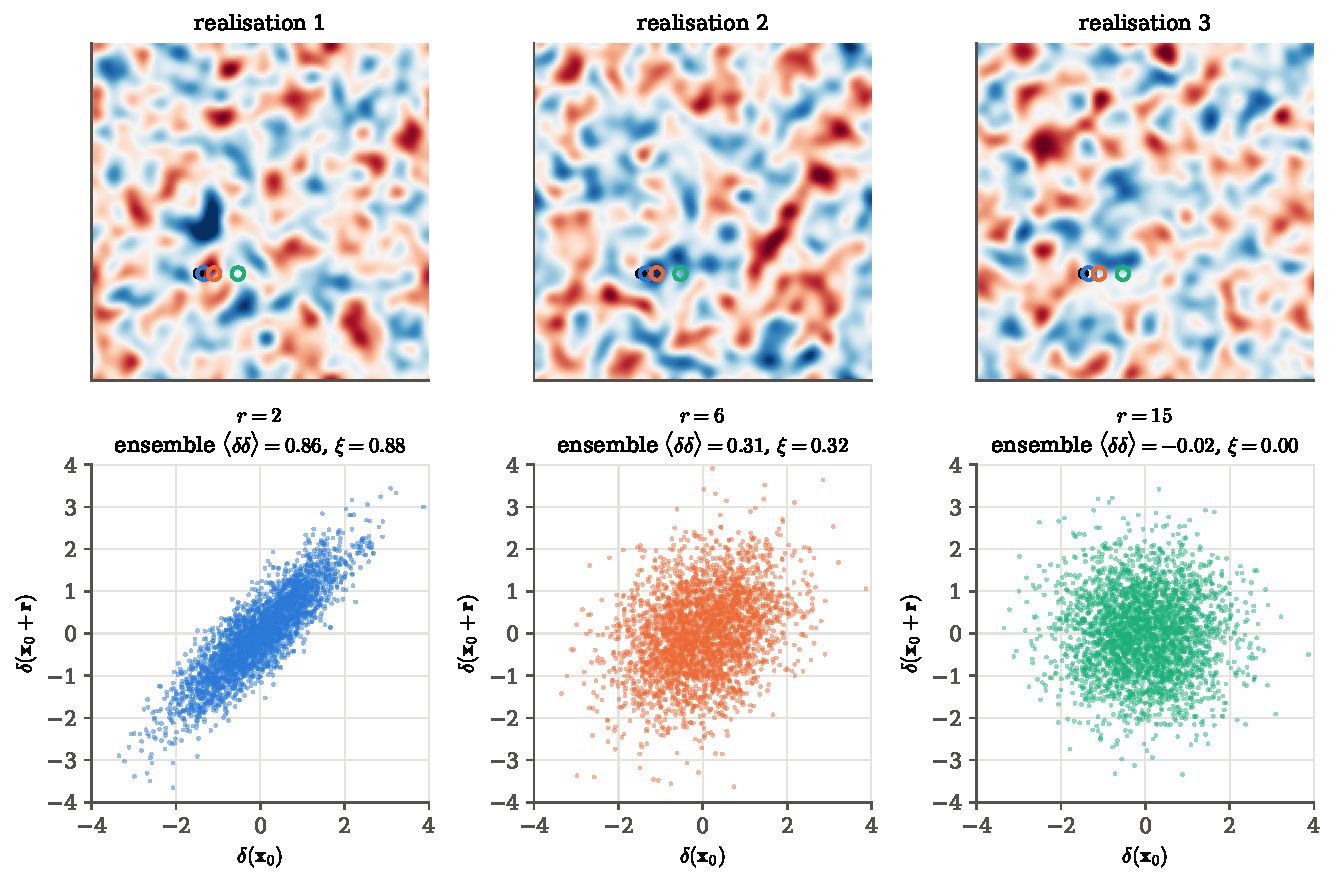
\includegraphics[width=\linewidth]{figures/ch07/ensemble_two_points.pdf}
\caption{Top: three universes drawn from the same Gaussian random field. The
black dot is the fixed point $\bm x_0$; the coloured circles are the points
$2$, $6$ and $15$ cells to its right. Bottom: the pair
$\bigl(\delta(\bm x_0),\delta(\bm x_0+\bm r)\bigr)$ collected over $3000$
universes. Close points rise and fall together, distant points are unrelated, and
the average of the product traces $\xi(r)$.}
\label{7a:fig:ensemble-sim}
\end{figure}

\begin{pitfall}[A correlation function is not a property of one map]
Each realisation in \cref{7a:fig:ensemble-sim} has its own hot and cold spots,
and in none of them is the field ``homogeneous'' in the everyday sense.
Homogeneity, isotropy and $\xi(r)$ are properties of the ensemble. Measuring them
from one map requires an extra assumption, ergodicity, and carries an
irreducible error (\cref{7a:sec:ergodic}).
\end{pitfall}

The correlation function squeezes a whole distribution over maps into one
function of one variable. How much of the distribution survives? In general,
very little: the $n$-point distributions can do almost anything that an average
over pairs does not see. But there is one large class of fields, and the most
important one in physics, for which $\xi$ captures everything.
\section{Gaussian random fields: when two points tell the whole story}
\label{7a:sec:grf}

A random field is specified by all of its $n$-point distributions, for every
$n$ and every placement of the points. That is an infinite amount of
information, and no experiment will ever pin it down. The microwave background
spares us this. To the precision of every test so far, its temperature
fluctuations are a \emph{Gaussian} field \srcref{HobsonBMC}{p.~229}, and for a
Gaussian field the infinite tower collapses to a single function: once we know
the mean and $\xi(r)$, we know every $n$-point distribution. This is why the
whole of CMB cosmology can be phrased in terms of a power spectrum.

\begin{workdef}[Gaussian random field]
A random field is \newterm{Gaussian} if for every finite set of points
$\bm x_1,\dots,\bm x_n$ the vector $\bm\delta=(\delta(\bm x_1),\dots,\delta(\bm x_n))$
has a multivariate Gaussian density
\unpack{the density of \cref{ch:02}, fixed by a mean vector and a covariance
matrix}. For a homogeneous, isotropic, zero-mean Gaussian field the covariance
matrix is read off the correlation function,
$\Cmat_{ij}=\xi(|\bm x_i-\bm x_j|)$, so
\begin{equation}
  p(\bm\delta)=\frac{1}{(2\pi)^{n/2}\sqrt{\det\Cmat}}\,
  \exp\Bigl(-\tfrac12\,\bm\delta\T\Cmat^{-1}\bm\delta\Bigr) .
  \label{7a:eq:grf}
\end{equation}
\emph{Consequence:} $\xi(r)$ determines every $n$-point distribution.
\end{workdef}

\Cref{7a:fig:points-matrix} shows the construction for three points. Write down
the three separations, look up $\xi$ at each, fill the symmetric matrix, and
\eqref{7a:eq:grf} is the joint density of the three field values. Nothing else
about the field enters. Consistency, the marginalisation condition in the
definition of a random field, holds automatically: integrating one variable out
of a multivariate Gaussian leaves the Gaussian of the remaining ones with the
corresponding sub-block of $\Cmat$ (\cref{ch:02}), which is exactly the matrix
we would have built for the smaller set of points.

\begin{figure}[htbp]
\centering
\begin{tikzpicture}[x=1cm,y=1cm]
  \fill[formblue!8] (0,0) rectangle (4.2,3);
  \coordinate (A) at (0.8,0.7);
  \coordinate (B) at (3.4,1.0);
  \coordinate (Cc) at (1.6,2.4);
  \draw[faint] (A) -- (B) node[midway,below,lbl] {$r_{12}$};
  \draw[faint] (A) -- (Cc) node[midway,left,lbl] {$r_{13}$};
  \draw[faint] (B) -- (Cc) node[midway,above right,lbl] {$r_{23}$};
  \fill[bdryred] (A) circle (2pt) node[anchor=north east,lbl] {$\bm x_1$};
  \fill[bdryred] (B) circle (2pt) node[anchor=north west,lbl] {$\bm x_2$};
  \fill[bdryred] (Cc) circle (2pt) node[anchor=south east,lbl] {$\bm x_3$};
  \node[lbl,align=center] at (8.3,1.5) {$\Cmat=\begin{pmatrix}
     \xi(0) & \xi(r_{12}) & \xi(r_{13})\\
     \xi(r_{12}) & \xi(0) & \xi(r_{23})\\
     \xi(r_{13}) & \xi(r_{23}) & \xi(0)\end{pmatrix}$};
  \node[lbl,align=center] at (8.3,0.05)
     {$\bigl(\delta(\bm x_1),\delta(\bm x_2),\delta(\bm x_3)\bigr)\sim\Normal(\bm 0,\Cmat)$};
\end{tikzpicture}
\caption{For a Gaussian field the joint distribution at any set of points is
built from the separations alone. Three points give three distances; the
correlation function at those distances fills the covariance matrix, and the
multivariate Gaussian with that matrix is the joint law of the three values.}
\label{7a:fig:points-matrix}
\end{figure}

\paragraph{Why so many physical fields are Gaussian.}
Three mechanisms recur, one at a time.
\emph{Many small causes.} When the value at a point is the sum of many small
independent contributions, as the voltage across a resistor sums the kicks of
many electrons, the central limit theorem (\cref{ch:02}) makes it Gaussian. The
same argument applied to the values at any finite set of points makes them
jointly Gaussian.
\emph{Quantum vacuum.} Quantum fluctuations of a free field in its vacuum state
are Gaussian, and the simplest models of inflation stretch exactly such
fluctuations to cosmological size.
\emph{Linear evolution.} A linear map $\mathbf A$ applied to a Gaussian vector
gives another Gaussian vector, with covariance $\mathbf A\Cmat\mathbf A\T$
(\cref{ch:01}). The CMB fluctuations have amplitude $10^{-5}$, so the equations
that evolve them are linear, and an initially Gaussian field stays Gaussian
\srcref{HobsonBMC}{p.~230}.
Gaussianity is lost when evolution is non-linear. Gravitational collapse turns
the nearly Gaussian early matter field into a skewed web of halos and filaments;
this is the regime where the linear and halofit spectra of \cref{ch:T1} part
company.

\subsection{What Gaussianity predicts}
\label{7a:sec:grf-predicts}

Because the whole distribution is fixed by $\xi$, a Gaussian field makes sharp
predictions that we can check on a map. We need three of them repeatedly.

\paragraph{The pair distribution.}
For two points a distance $r$ apart, \eqref{7a:eq:grf} with $n=2$ is a
bivariate Gaussian. After dividing each value by $\sigma$ (so both have unit
variance), its correlation coefficient is $\rho(r)=\xi(r)/\sigma^2$, with
$\sigma^2=\xi(0)$ the variance at a point. Its contours are ellipses along the diagonal, narrow
when $\rho$ is near $1$ and circular when $\rho=0$
(\cref{7a:fig:gaussian-checks}, left). These are the clouds of
\cref{7a:fig:ensemble-sim}, now drawn from the formula.

\paragraph{The field around a hot spot.}
\emph{What we observed.} A point where the field is high,
$\delta(\bm x)=\nu\sigma$: the field sits $\nu$ standard deviations above its
mean. \emph{The question.} What should we expect a distance $r$ away?
\emph{The idea.} Split the second value into a part that the first value
predicts and a remainder $Z$ that it says nothing about,
\begin{equation*}
  \delta(\bm x+\bm r)=\frac{\xi(r)}{\sigma^2}\,\delta(\bm x)+Z .
\end{equation*}
This equation defines $Z$, and the coefficient $\xi(r)/\sigma^2$ is chosen so
that $Z$ is uncorrelated with $\delta(\bm x)$:
$\Cov(Z,\delta(\bm x))=\xi(r)-\frac{\xi(r)}{\sigma^2}\sigma^2=0$. $Z$ is a linear
combination of the Gaussian pair, so $Z$ and $\delta(\bm x)$ are jointly
Gaussian, and for jointly Gaussian variables uncorrelated means independent.
Knowing $\delta(\bm x)$ therefore tells us nothing about $Z$, and
\begin{align}
  \E\bigl[\delta(\bm x+\bm r)\given\delta(\bm x)=\nu\sigma\bigr]
  &\eqby{1}\frac{\xi(r)}{\sigma^2}\,\nu\sigma+\E[Z]
   \eqby{2}\nu\sigma\,\frac{\xi(r)}{\sigma^2},
  \label{7a:eq:condmean}\\
  \Var\bigl[\delta(\bm x+\bm r)\given\delta(\bm x)=\nu\sigma\bigr]
  &\eqby{3}\Var Z
   \eqby{4}\sigma^2-\frac{\xi(r)^2}{\sigma^2} .
  \nonumber
\end{align}
\begin{explain}
  \item Conditioning on $\delta(\bm x)=\nu\sigma$ fixes the first term; $Z$ is
        independent of $\delta(\bm x)$, so its distribution is unchanged.
  \item $Z$ is a combination of zero-mean variables.
  \item The first term is fixed by the condition, so only $Z$ fluctuates.
  \item $\Var Z=\Var\delta(\bm x+\bm r)-\frac{\xi^2}{\sigma^4}\Var\delta(\bm x)
        =\sigma^2-\xi^2/\sigma^2$, using the independence just shown.
\end{explain}
\emph{What it means.} The mean profile around a point of height $\nu\sigma$ is the
correlation function itself, scaled by $\nu/\sigma$: a hot spot is surrounded by
warm field out to the correlation length. This is the seed of the theory of
peaks and clusters in \cite{BBKS1986}. If instead of a single height we select
all points above a threshold, $\delta>\nu\sigma$, we average
\eqref{7a:eq:condmean} over the heights of the selected points (the tower
property of expectation). The conditional mean is proportional to the height, so
the average simply replaces $\nu\sigma$ by the mean height $\bar\nu\sigma$ of the
selected points.

The script \pyname{code/ch07/02_gaussian_checks.py} tests this on one $512\times512$
map with $\xi=e^{-r^2/2\ell^2}$, $\ell=4$. A fraction $\SevAHotFrac$ of the pixels
exceed $2\sigma$ (the Gaussian tail gives $0.0228$), and their mean height is
$\bar\nu=\SevACondNubar$ (the Gaussian value is
$\varphi(2)/[1-\Phi(2)]=2.373$, with $\varphi$ and $\Phi$ the standard normal density
and CDF). Four cells to their right the average field is $\SevACondProfFour$, against
$\bar\nu\,\xi(4)/\sigma^2=\SevACondTheoFour$, and the whole profile follows
\eqref{7a:eq:condmean} (\cref{7a:fig:gaussian-checks}, middle). The small excess at
large $r$ is noise: the selected pixels belong to a few hundred hot spots, so the
average beyond the correlation length scatters by about $1/\sqrt{\text{a few
hundred}}\approx0.05$.

\paragraph{Four-point moments from two-point ones.}
A Gaussian field carries no new information at higher order: every moment is
built from $\xi$. \emph{The question.} What is the average of a product of four
field values? \emph{The tool.} The moment generating function of a zero-mean
Gaussian vector (\cref{ch:01,ch:02}),
$\E\bigl[e^{\bm t\T\bm\delta}\bigr]=e^{\frac12\bm t\T\Cmat\bm t}$. Expand both
sides in powers of $\bm t$: on the left each coefficient is a moment, on the
right it is built from $\Cmat$ alone. Matching coefficients gives the answer.
For four field values
$\delta_1,\dots,\delta_4$ (not necessarily at distinct points) and
$C_{ij}=\langle\delta_i\delta_j\rangle$:
\begin{align}
  \langle\delta_1\delta_2\delta_3\delta_4\rangle
  &\eqby{1}\Bigl[\text{coefficient of }t_1t_2t_3t_4\text{ in }
     \E\,e^{\bm t\T\bm\delta}\Bigr]
   \eqby{2}\Bigl[\text{coefficient of }t_1t_2t_3t_4\text{ in }
     \tfrac{1}{2!}\bigl(\tfrac12\textstyle\sum_{ij}C_{ij}t_it_j\bigr)^2\Bigr]
   \nonumber\\
  &\eqby{3}\tfrac18\cdot 8\,\bigl(C_{12}C_{34}+C_{13}C_{24}+C_{14}C_{23}\bigr)
   \eqby{4}C_{12}C_{34}+C_{13}C_{24}+C_{14}C_{23} .
  \label{7a:eq:wick}
\end{align}
\begin{explain}
  \item Expanding $e^{\bm t\T\bm\delta}$, the term $t_1t_2t_3t_4$ appears only
        from $\frac{1}{4!}(\bm t\T\bm\delta)^4$, where it occurs $4!$ times with
        coefficient $\delta_1\delta_2\delta_3\delta_4$; so its coefficient in the
        average is the four-point moment.
  \item In $e^{\frac12\bm t\T\Cmat\bm t}=1+\frac12\bm t\T\Cmat\bm t
        +\frac1{2!}(\frac12\bm t\T\Cmat\bm t)^2+\dots$ only the quadratic power of
        the exponent has terms of fourth order in $\bm t$.
  \item $(\sum_{ij}C_{ij}t_it_j)^2=\sum_{ijkl}C_{ij}C_{kl}t_it_jt_kt_l$. The term
        $t_1t_2t_3t_4$ arises when $(i,j,k,l)$ is an ordering of $(1,2,3,4)$:
        $24$ orderings, which split the four indices into one of the three
        pairings, each pairing reached in $2\times2\times2=8$ ways (which pair
        comes first, and the order inside each pair). The prefactor is
        $\frac12\cdot\frac14=\frac18$.
  \item Simplify.
\end{explain}
This is \newterm{Isserlis' theorem}, called Wick's theorem in field theory: the
four-point function is the sum over the three ways of pairing the points, and
every odd moment vanishes (the exponent is even in $\bm t$). Setting
$\delta_3=\delta_1$ and $\delta_4=\delta_2$ at two points a distance $r$ apart,
\begin{equation}
  \langle\delta(\bm x)^2\,\delta(\bm x+\bm r)^2\rangle=\sigma^4+2\,\xi(r)^2 ,
  \label{7a:eq:wick-pair}
\end{equation}
and at $r=0$ this is the familiar $\langle\delta^4\rangle=3\sigma^4$ of a single
Gaussian. Equation \eqref{7a:eq:wick-pair} gives a test of Gaussianity that needs
nothing but the map: measure both sides and compare. For the Gaussian map the ratio of the two sides is
$\SevAWickGaussZero$ at $r=0$ and $\SevAWickGaussSix$ at $r=6$. For a lognormal
field, $y=e^{0.8\,\delta}$ standardised to zero mean and unit variance, a common
model for the non-linear matter density, the same ratio is $\SevAWickLogZero$ at
$r=0$ and $\SevAWickLogSix$ at $r=6$ (\cref{7a:fig:gaussian-checks}, right). The
lognormal field has a perfectly good two-point function, but that function no
longer predicts its four-point function: the lognormal field carries information
beyond $\xi$.

\begin{figure}[htbp]
\centering
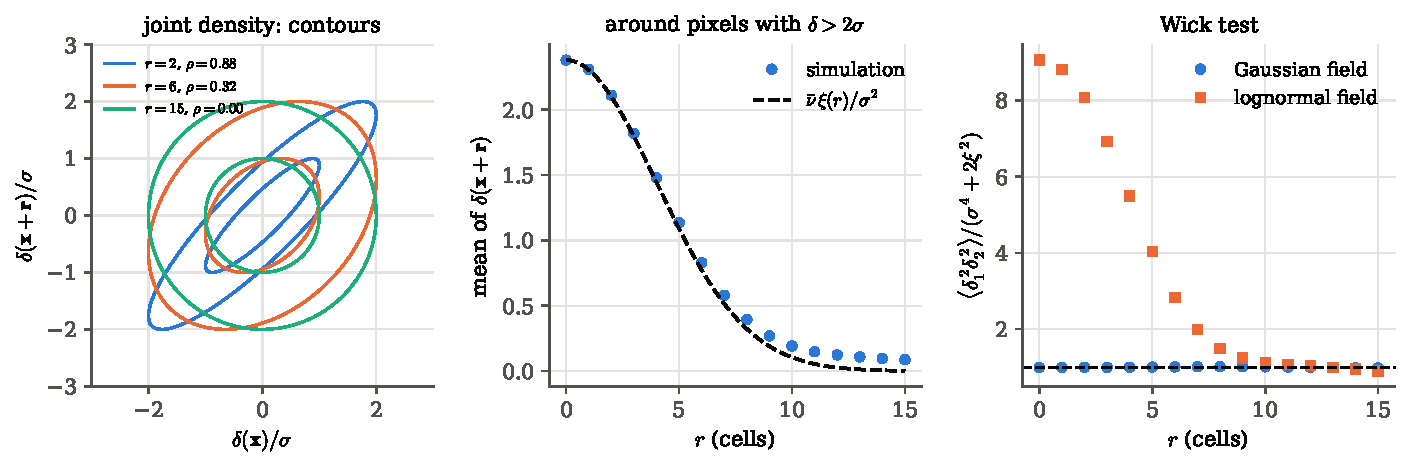
\includegraphics[width=\linewidth]{figures/ch07/gaussian_checks.pdf}
\caption{Three predictions of Gaussianity. Left: the $1\sigma$ and $2\sigma$
contours of the joint density of the field at two points, for three separations.
Middle: the mean field at distance $r$ from pixels above $2\sigma$ (dots)
follows the scaled correlation function (dashed). Right: the four-point moment
$\langle\delta_1^2\delta_2^2\rangle$ divided by its Gaussian prediction
$\sigma^4+2\xi^2$ is $1$ for a Gaussian map and far from $1$ for a lognormal map.}
\label{7a:fig:gaussian-checks}
\end{figure}

\begin{keyidea}[For a Gaussian field, $\xi(r)$ is everything]
A homogeneous, isotropic Gaussian random field is completely specified by its
mean and its correlation function. All $n$-point distributions follow from
\eqref{7a:eq:grf}, all higher moments are sums over pairings
\eqref{7a:eq:wick}, and the conditional field around any feature is a linear
function of $\xi$. A summary that captures $\xi$ (or its Fourier transform)
loses nothing. For a non-Gaussian field the same summary is incomplete.
\end{keyidea}

The part of the four-point function that is \emph{not} the sum over pairings,
$\langle\delta_1\delta_2\delta_3\delta_4\rangle-(C_{12}C_{34}+C_{13}C_{24}+C_{14}C_{23})$,
is called the connected four-point function; its Fourier transform is the
trispectrum, and the Fourier transform of the three-point function is the
bispectrum. They are the ``higher-order'' row of the taxonomy in
\cref{7a:sec:phases}, and they vanish identically for a Gaussian field.

From here on the working model is a homogeneous, isotropic Gaussian field, whose
one free function is $\xi(r)$. In pixel variables its covariance matrix
$\Cmat_{ij}=\xi(|\bm x_i-\bm x_j|)$ is full: every pixel is correlated with its
neighbours. The natural question is whether some other set of variables makes
that matrix diagonal, so that the variables are independent.
\section{Fourier modes and the power spectrum}
\label{7a:sec:fourier}

A Gaussian map of a million pixels is a Gaussian vector with a million-by-million
covariance matrix. To simulate it with the Cholesky factor of \cref{ch:06} costs
about $n^3/3\approx3\times10^{17}$ operations, and to evaluate its likelihood
\eqref{7a:eq:grf} needs the inverse and the determinant of the same matrix. Both
are hopeless. Yet the matrix is far from arbitrary: by homogeneity, every entry
depends only on the separation of the two pixels. That structure is enough to
diagonalise it without computing anything.

\paragraph{The question.} In which variables is a homogeneous field a set of
\emph{uncorrelated} random numbers, and what are their variances?

\emph{The general tool.} Any set of correlated random variables $x_j$ with a
symmetric covariance matrix $V$ can be rotated into uncorrelated ones,
$y_i=\sum_jA_{ij}x_j$: take the rows of $A$ to be the eigenvectors of $V$. The
variances of the $y_i$ are then the eigenvalues of $V$
\srcref{Cowan}{\S1.7, (1.61)--(1.65)}. For a general matrix the eigenvectors
must be found numerically.
\emph{The homogeneous case.} Here we know the eigenvectors in advance: they are
plane waves. The reason is the one familiar from physics. A Hamiltonian that is
unchanged by translations commutes with the translation operator, so both can be
diagonalised together, by momentum eigenstates $e^{i\bm k\cdot\bm x}$. For the
same reason the normal modes of a uniform chain of masses and springs are waves.
A homogeneous covariance is also unchanged by translations, so its eigenvectors
are plane waves too.

\subsection{Four pixels by hand}
\label{7a:sec:circulant}

Take a ring of $n=4$ pixels, a periodic line so that pixel $4$ is pixel $0$
again. Homogeneity says the covariance of pixels $i$ and $j$ is $\xi$ of their
distance around the ring, so with $\xi_0=\xi(0)$, $\xi_1=\xi(1)$ and
$\xi_2=\xi(2)$,
\begin{equation*}
  \Cmat=\begin{pmatrix}
    \xi_0&\xi_1&\xi_2&\xi_1\\
    \xi_1&\xi_0&\xi_1&\xi_2\\
    \xi_2&\xi_1&\xi_0&\xi_1\\
    \xi_1&\xi_2&\xi_1&\xi_0
  \end{pmatrix}.
\end{equation*}
Each row is the row above shifted one place to the right, with wrap-around: a
\newterm{circulant} matrix. Try the plane wave $e^{(m)}_j=e^{2\pi i\,jm/4}$,
$j=0,\dots,3$, for an integer wavenumber $m$. Its first component after
multiplication by $\Cmat$ is
\begin{align*}
  (\Cmat e^{(m)})_0
  &=\xi_0+\xi_1e^{2\pi i m/4}+\xi_2e^{2\pi i\,2m/4}+\xi_1e^{2\pi i\,3m/4}
   \eqby{1}\xi_0+2\xi_1\cos\frac{\pi m}{2}+\xi_2\cos(\pi m),
\end{align*}
\begin{explain}
  \item $e^{2\pi i\,3m/4}=e^{-2\pi i m/4}$, so the two $\xi_1$ terms add to
        $2\xi_1\cos(\pi m/2)$; and $e^{i\pi m}=\cos\pi m$ is real.
\end{explain}
and every other row gives the same number times $e^{(m)}_j$, because row $j$ is
row $0$ shifted by $j$ and the plane wave picks up exactly the factor
$e^{2\pi i jm/4}$ under that shift. So $\Cmat e^{(m)}=\lambda_me^{(m)}$ with
\begin{equation*}
  \lambda_0=\xi_0+2\xi_1+\xi_2,\qquad
  \lambda_1=\lambda_3=\xi_0-\xi_2,\qquad
  \lambda_2=\xi_0-2\xi_1+\xi_2 .
\end{equation*}
With $\xi_0=1$, $\xi_1=0.5$, $\xi_2=0.2$ the eigenvalues are $2.2$, $0.8$, $0.2$,
$0.8$. They are the variances of the four Fourier coefficients of the map:
large for the smooth mode $m=0$, small for the zig-zag mode $m=2$, because
neighbouring pixels are positively correlated and the zig-zag fights that
correlation.

The eigenvalues also tell us whether a proposed $\xi$ is possible at all. Try
$\xi_0=1$, $\xi_1=0.9$, $\xi_2=0$: neighbours very strongly correlated,
next-neighbours not at all. It looks harmless, and $|\xi|\le\xi_0$ holds. But
$\lambda_2=1-1.8=-0.8<0$, a negative variance, so no random field has this
correlation function. In words: if pixels $0,1$ are correlated at $0.9$ and
pixels $1,2$ are too, then pixels $0$ and $2$ cannot be uncorrelated. The
eigenvalues are the positivity test \eqref{7a:eq:posdef} made explicit.

\Cref{7a:fig:circulant} summarises the construction, and
\pyname{code/ch07/03_fourier_diagonal.py} repeats it on a ring of $n=64$ pixels
with $\xi(r)=e^{-r^2/2\ell^2}$, $\ell=3$. Rotating the $64\times64$ covariance
matrix into the Fourier basis leaves it diagonal: the largest off-diagonal entry
is $\SevAOffDiagExact$, rounding error. The diagonal agrees with the discrete
Fourier transform of the first row of $\Cmat$, and with the eigenvalues of $\Cmat$
from a general-purpose eigensolver, to $\SevADiagMatch$. As a statistical check
the script then draws $M=\SevAM$ rings with the Cholesky factor, a method that
knows nothing about Fourier modes, Fourier transforms each one, and estimates the
correlation coefficients between different modes. Over the $\SevANBig$ modes that
carry appreciable power their r.m.s.\ is $\SevAOffDiagRMS$, which is the
$1/\sqrt M=\SevANoiseExpect$ expected for truly uncorrelated variables
(\cref{7a:fig:fourier-diagonal}).

\begin{figure}[htbp]
\centering
\begin{tikzpicture}[x=0.5cm,y=0.5cm]
  \foreach \i in {0,...,3}{\foreach \j in {0,...,3}{
    \pgfmathtruncatemacro{\d}{min(abs(\i-\j),4-abs(\i-\j))}
    \pgfmathsetmacro{\shade}{\d==0 ? 70 : (\d==1 ? 40 : 15)}
    \fill[formblue!\shade] (\j,-\i) rectangle ++(1,-1);
    \draw[faint] (\j,-\i) rectangle ++(1,-1);}}
  \node[lbl] at (2,0.7) {pixel space: $\Cmat_{ij}=\xi(|i-j|)$};
  \node[lbl] at (2,-4.7) {every entry nonzero};
  \draw[->,thick,accent] (5.3,-2) -- (8.7,-2);
  \node[lbl,align=center] at (7,-0.9) {rotate by\\ plane waves};
  \begin{scope}[xshift=9.5cm]
  \foreach \i/\v in {0/70,1/30,2/8,3/30}{
    \foreach \j in {0,...,3}{\draw[faint] (\j,-\i) rectangle ++(1,-1);}
    \fill[fibreorange!\v] (\i,-\i) rectangle ++(1,-1);}
  \node[lbl] at (2,0.7) {Fourier space: $\lambda_m\delta_{mm'}$};
  \node[lbl] at (2,-4.7) {diagonal: $\lambda_m=$ DFT of $\xi$};
  \end{scope}
\end{tikzpicture}
\caption{A homogeneous covariance on a ring of four pixels. Left: in pixel space
every pixel is correlated with every other (darker means larger $\xi$). Right:
in the basis of plane waves the same matrix is diagonal, and the diagonal entries,
the variances of the Fourier modes, are the discrete Fourier transform of the
correlation function.}
\label{7a:fig:circulant}
\end{figure}

\begin{figure}[htbp]
\centering
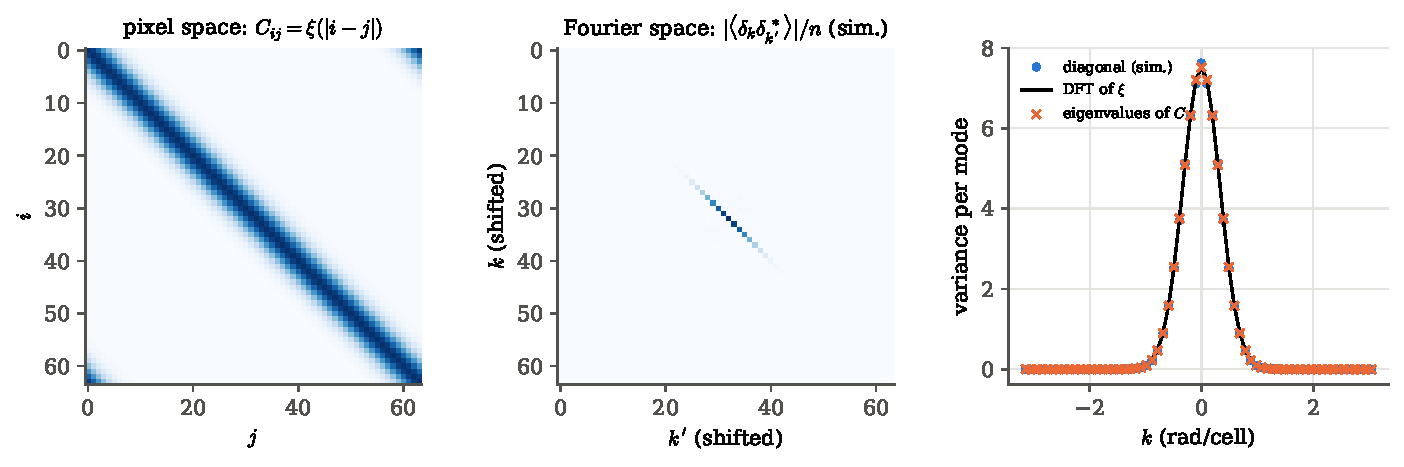
\includegraphics[width=\linewidth]{figures/ch07/fourier_diagonal.pdf}
\caption{The same statement for $64$ pixels. Left: the covariance matrix in
pixel space, a band of width a few correlation lengths. Middle: the covariance
of the Fourier coefficients, estimated from $20\,000$ simulated rings, is
diagonal. Right: the diagonal (dots) equals the discrete Fourier transform of
$\xi$ (line), and both equal the eigenvalues of $\Cmat$ (crosses).}
\label{7a:fig:fourier-diagonal}
\end{figure}

\subsection{The continuum: why Fourier modes are uncorrelated}
\label{7a:sec:wk}

The same calculation works in any dimension $d$ and in the continuum. We fix a
Fourier convention for the whole chapter:
\begin{equation}
  \delta_{\bm k}=\int\dd^dx\;\delta(\bm x)\,e^{-i\bm k\cdot\bm x},
  \qquad
  \delta(\bm x)=\int\frac{\dd^dk}{(2\pi)^d}\;\delta_{\bm k}\,e^{i\bm k\cdot\bm x},
  \label{7a:eq:ft}
\end{equation}
with the useful identity $\int\dd^dx\,e^{-i(\bm k-\bm k')\cdot\bm x}
=(2\pi)^d\delta_D(\bm k-\bm k')$, where $\delta_D$ is the Dirac delta. Because
$\delta(\bm x)$ is real, complex conjugating the first relation gives the
\newterm{reality condition}
\begin{equation}
  \delta_{\bm k}^*=\delta_{-\bm k},
  \label{7a:eq:reality}
\end{equation}
so the modes $\bm k$ and $-\bm k$ are not independent numbers: one is the
complex conjugate of the other \srcref{HobsonBMC}{p.~132}. Now compute the
covariance of two Fourier coefficients of a homogeneous field:
\begin{align}
  \langle\delta_{\bm k}\,\delta_{\bm k'}^*\rangle
  &\eqby{1}\int\dd^dx\int\dd^dy\;\langle\delta(\bm x)\delta(\bm y)\rangle\,
     e^{-i\bm k\cdot\bm x+i\bm k'\cdot\bm y}
   \nonumber\\
  &\eqby{2}\int\dd^dx\int\dd^dy\;\xi(\bm x-\bm y)\,
     e^{-i\bm k\cdot\bm x+i\bm k'\cdot\bm y}
   \nonumber\\
  &\eqby{3}\int\dd^dy\;e^{-i(\bm k-\bm k')\cdot\bm y}
     \int\dd^dr\;\xi(\bm r)\,e^{-i\bm k\cdot\bm r}
   \nonumber\\
  &\eqby{4}(2\pi)^d\,\delta_D(\bm k-\bm k')\,P(\bm k),
  \qquad
  P(\bm k)\equiv\int\dd^dr\;\xi(\bm r)\,e^{-i\bm k\cdot\bm r} .
  \label{7a:eq:wk}
\end{align}
\begin{explain}
  \item Insert \eqref{7a:eq:ft} for $\delta_{\bm k}$ and for $\delta_{\bm k'}^*$
        (whose exponent changes sign), and take the ensemble average inside the
        integrals, where only the fields are random.
  \item Homogeneity: the average of the product depends only on $\bm x-\bm y$,
        \eqref{7a:eq:homog}.
  \item Change variables from $(\bm x,\bm y)$ to $(\bm r=\bm x-\bm y,\bm y)$, a shift
        with unit Jacobian. The exponent becomes
        $-i\bm k\cdot(\bm r+\bm y)+i\bm k'\cdot\bm y
        =-i\bm k\cdot\bm r-i(\bm k-\bm k')\cdot\bm y$, which factorises.
  \item The $\bm y$ integral is the Dirac-delta identity; the $\bm r$ integral is a
        function of $\bm k$ alone, which we name $P(\bm k)$.
\end{explain}
Two Fourier modes with different wavevectors are uncorrelated. The reason is the
$\bm y$ integral, the integral over where the pair of points sits: it averages
the phase $e^{-i(\bm k-\bm k')\cdot\bm y}$ to zero unless $\bm k=\bm k'$.
Homogeneity is used in exactly one place, step (2); without it the $\bm y$
integral would not split off. The variance of each mode is the \newterm{power
spectrum} $P(\bm k)$, the Fourier transform of $\xi$. Using the reality
condition to replace $\delta_{\bm k'}^*$ by $\delta_{-\bm k'}$, the same result
reads $\langle\delta_{\bm k}\delta_{\bm k'}\rangle=(2\pi)^d\delta_D(\bm k+\bm k')P(k)$,
the form in which cosmology usually defines the matter power spectrum.
Inverting the Fourier transform in \eqref{7a:eq:wk} gives $\xi$ back.

\begin{keyidea}[Wiener--Khinchin: the power spectrum is the Fourier transform of $\xi$]
For a statistically homogeneous field, different Fourier modes are uncorrelated,
\begin{gather*}
  \langle\delta_{\bm k}\,\delta_{\bm k'}^*\rangle=(2\pi)^d\,\delta_D(\bm k-\bm k')\,P(\bm k),\\
  P(\bm k)=\int\dd^dr\,\xi(\bm r)\,e^{-i\bm k\cdot\bm r},
  \qquad
  \xi(\bm r)=\int\frac{\dd^dk}{(2\pi)^d}\,P(\bm k)\,e^{i\bm k\cdot\bm r}.
\end{gather*}
Isotropy makes $P$ depend only on $k=|\bm k|$. The power spectrum is the
variance per Fourier mode, so $P(k)\ge0$, and a function is a valid correlation
function if and only if its Fourier transform is non-negative.
\end{keyidea}

The last sentence is Bochner's theorem; the four-pixel example above is its
smallest case. It has two directions. \emph{Valid $\xi$ implies $P\ge0$:} this is
immediate from \eqref{7a:eq:wk}, since $P$ is a variance. \emph{$P\ge0$ implies a
valid $\xi$:} here the proof is a construction, the simulation recipe of
\cref{7a:sec:simulate}, which takes any $P\ge0$ and builds a field that has it.

A remark on conventions. Some cosmology texts use the symmetric convention, with
$(2\pi)^{-d/2}$ on each side of the transform; then
$\langle\delta_{\bm k}\delta_{\bm k'}^*\rangle=\delta_D(\bm k-\bm k')P(k)$ with
the \emph{same} $P(k)$, because the relation between $P$ and $\xi$ is unchanged
(\cref{ch:T1}). This is the $P(k)$ that CAMB returns.

\emph{How the variance splits among the modes.} Setting $\bm r=0$ in the inverse
transform,
\begin{equation}
  \sigma^2=\xi(0)=\int\frac{\dd^dk}{(2\pi)^d}\,P(k),
  \label{7a:eq:sigma2}
\end{equation}
so the variance of the field is the sum of the variances of its modes, and
$P(k)\,\dd^dk/(2\pi)^d$ is the share of the variance carried by the modes in
$\dd^dk$. In three dimensions with isotropy, $\dd^3k=4\pi k^2\dd k$, and
\begin{equation*}
  \sigma^2=\int_0^\infty\frac{\dd k}{k}\,\Delta^2(k),
  \qquad
  \Delta^2(k)\equiv\frac{k^3P(k)}{2\pi^2},
\end{equation*}
the \newterm{dimensionless power spectrum}: the variance per logarithmic interval
of $k$ (in two dimensions the same reasoning gives $\Delta^2=k^2P/2\pi$). A
spectrum with constant $\Delta^2$ puts equal variance in every octave of scale.
The primordial curvature perturbation of inflation is close to this
``scale-invariant'' case.

\paragraph{Isotropic transforms in three and two dimensions.}
For an isotropic field the angular part of the Fourier integral can be done once
and for all. In three dimensions, put the $k_z$ axis along $\bm r$, so
$\bm k\cdot\bm r=kr\cos\theta$:
\begin{align}
  \xi(r)
  &\eqby{1}\int_0^\infty\frac{k^2\dd k}{(2\pi)^3}\,P(k)\int_0^{2\pi}\dd\phi
     \int_{-1}^{1}\dd(\cos\theta)\,e^{ikr\cos\theta}
   \eqby{2}\int_0^\infty\frac{k^2\dd k}{(2\pi)^3}\,P(k)\;2\pi\,\frac{2\sin kr}{kr}
   \nonumber\\
  &=\int_0^\infty\frac{k^2\dd k}{2\pi^2}\,P(k)\,\frac{\sin kr}{kr} ,
  \label{7a:eq:xi3d}
\end{align}
\begin{explain}
  \item Spherical coordinates in $\bm k$-space, $\dd^3k=k^2\dd k\,\dd\phi\,\dd(\cos\theta)$,
        and $P$ depends only on $k$.
  \item $\int_{-1}^{1}e^{ikru}\dd u=\frac{e^{ikr}-e^{-ikr}}{ikr}=\frac{2\sin kr}{kr}$.
\end{explain}
the standard relation between $\xi$ and $P$ in cosmology. In two dimensions, with polar
angle $\phi$ between $\bm k$ and $\bm r$,
\begin{equation}
  \xi(r)=\int_0^\infty\frac{k\,\dd k}{(2\pi)^2}\,P(k)\int_0^{2\pi}e^{ikr\cos\phi}\dd\phi
  =\int_0^\infty\frac{k\,\dd k}{2\pi}\,P(k)\,J_0(kr),
  \label{7a:eq:xi2d}
\end{equation}
using the integral representation of the Bessel function,
$J_0(x)=\frac1{2\pi}\int_0^{2\pi}e^{ix\cos\phi}\dd\phi$. The inverse relations are
the same with the roles of $P$ and $\xi$ exchanged and the factors of $2\pi$
moved: $P(k)=4\pi\int_0^\infty r^2\dd r\,\xi(r)\frac{\sin kr}{kr}$ in 3D and
$P(k)=2\pi\int_0^\infty r\,\dd r\,\xi(r)J_0(kr)$ in 2D. On the sphere the analogue
is the Legendre series $C(\theta)=\sum_\ell\frac{2\ell+1}{4\pi}\Cell P_\ell(\cos\theta)$
\srcref{HobsonBMC}{(10.4)}, with the multipole $\ell$ playing the role of $k$.

\paragraph{Example: the Gaussian pair.}
Take $\xi(r)=\sigma^2e^{-r^2/2\ell^2}$ in $d$ dimensions. The Fourier integral
factorises over Cartesian components:
\begin{align}
  P(k)
  &\eqby{1}\sigma^2\prod_{a=1}^{d}\int_{-\infty}^{\infty}\dd r_a\,
     e^{-r_a^2/2\ell^2-ik_ar_a}
   \eqby{2}\sigma^2\prod_{a=1}^{d}\sqrt{2\pi\ell^2}\,e^{-k_a^2\ell^2/2}
   \eqby{3}\sigma^2\,(2\pi\ell^2)^{d/2}\,e^{-k^2\ell^2/2} .
  \label{7a:eq:gauss-pair}
\end{align}
\begin{explain}
  \item $r^2=\sum_ar_a^2$ and $\bm k\cdot\bm r=\sum_ak_ar_a$, so the exponential is
        a product of one-dimensional factors.
  \item Complete the square: $-\frac{r_a^2}{2\ell^2}-ik_ar_a
        =-\frac{(r_a+ik_a\ell^2)^2}{2\ell^2}-\frac{k_a^2\ell^2}{2}$, and the shifted
        Gaussian integral is $\sqrt{2\pi\ell^2}$.
  \item Multiply the $d$ factors; $\sum_ak_a^2=k^2$.
\end{explain}
A Gaussian of width $\ell$ in real space is a Gaussian of width $1/\ell$ in
Fourier space: a field correlated over $\ell$ has its power at $k\lesssim1/\ell$.
The $2$D version, $P=2\pi\ell^2\sigma^2e^{-k^2\ell^2/2}$, is the spectrum used in
\cref{7a:fig:ensemble-sim,7a:fig:gaussian-checks}. As a check of
\eqref{7a:eq:sigma2}, $\int\frac{\dd^2k}{(2\pi)^2}P
=\frac{2\pi\ell^2\sigma^2}{(2\pi)^2}\cdot\frac{2\pi}{\ell^2}=\sigma^2$.

\paragraph{Example: the exponential in two dimensions.}
For $\xi(r)=\sigma^2e^{-r/\ell}$ the 2D inverse relation needs
$\int_0^\infty r\,e^{-ar}J_0(kr)\,\dd r$ with $a=1/\ell$. Start from the Laplace
transform of $J_0$, $\int_0^\infty e^{-ar}J_0(kr)\,\dd r=(a^2+k^2)^{-1/2}$, and
differentiate both sides with respect to $a$:
\begin{align*}
  -\int_0^\infty r\,e^{-ar}J_0(kr)\,\dd r=-\frac{a}{(a^2+k^2)^{3/2}}
  \quad\Rightarrow\quad
  P(k)=2\pi\sigma^2\frac{a}{(a^2+k^2)^{3/2}}
  =\frac{2\pi\ell^2\sigma^2}{(1+k^2\ell^2)^{3/2}} .
\end{align*}
The kink of $e^{-r/\ell}$ at $r=0$ shows up as a power-law tail $P\propto k^{-3}$
at large $k$: a correlation function that is not smooth at the origin means a
field with structure on all small scales (\cref{7a:fig:pk-xi}, panel b). The
script \pyname{code/ch07/04_pk_xi_pairs.py} evaluates \eqref{7a:eq:xi2d}
numerically up to $k_{\max}=10$. For the Gaussian pair it reproduces the analytic
$\xi$ to $\SevAHankelErrA$. For the exponential the largest error is
$\SevAHankelErrB$, at $r=0$, and it has a clean explanation: the truncated tail
carries the variance
$\int_{k_{\max}}^\infty\frac{k\,\dd k}{2\pi}\frac{2\pi\ell^2}{(k\ell)^3}
=\frac{1}{\ell k_{\max}}=0.025$ for $\ell=4$ cells and $\sigma=1$.

\paragraph{Example: a preferred wavelength.}
If $P(k)$ is a narrow bump around $k_0$, nearly all the variance sits in waves of
wavelength $2\pi/k_0$, and \eqref{7a:eq:xi2d} gives $\xi(r)\approx\sigma^2J_0(k_0r)$
times a slowly decaying envelope. The correlation function oscillates and goes
\emph{negative}: a hot spot is surrounded by a cold ring at distance
$r\approx3.83/k_0$, the first minimum of $J_0$. For $k_0=0.5$ the minimum sits at
$\SevABandRMinJ$ cells, and the numerical transform puts it at $\SevABandRMin$
with $\xi=\SevABandXiMin$. The field looks like a pattern of cells and stripes, the
look of convection rolls or of a Turing pattern (\cref{7a:fig:pk-xi}, panel c). The
baryon acoustic oscillations are a weak version of the same thing: wiggles in
$P(k)$ become a bump in $\xi(r)$ at the sound horizon (\cref{ch:T1}).

\paragraph{Example: power laws.}
For $P(k)=Ak^n$ the substitution $u=kr$ in \eqref{7a:eq:xi3d} gives
$\xi(r)=\frac{A}{2\pi^2}r^{-(n+3)}\int_0^\infty u^{n+2}\frac{\sin u}{u}\dd u$, so
$\xi\propto r^{-(n+3)}$, and in $d$ dimensions $\xi\propto r^{-(n+d)}$. The
$u$ integral converges only for $-3<n<-1$ in 3D. Near $u=0$ the integrand is
about $u^{n+2}$, which needs $n>-3$; at large $u$ it oscillates with amplitude
$u^{n+1}$, which needs $n<-1$. For $n\le-3$ the trouble is at small $k$, the
largest scales; for $n\ge-1$ it is at large $k$, the smallest scales. Either way
the spectrum must be cut off, by the size of the survey or by smoothing. Steep
spectra (very negative $n$) give fields dominated by large waves; shallow ones
look like noise (\cref{7a:fig:simulate-2d} below).

\begin{figure}[htbp]
\centering
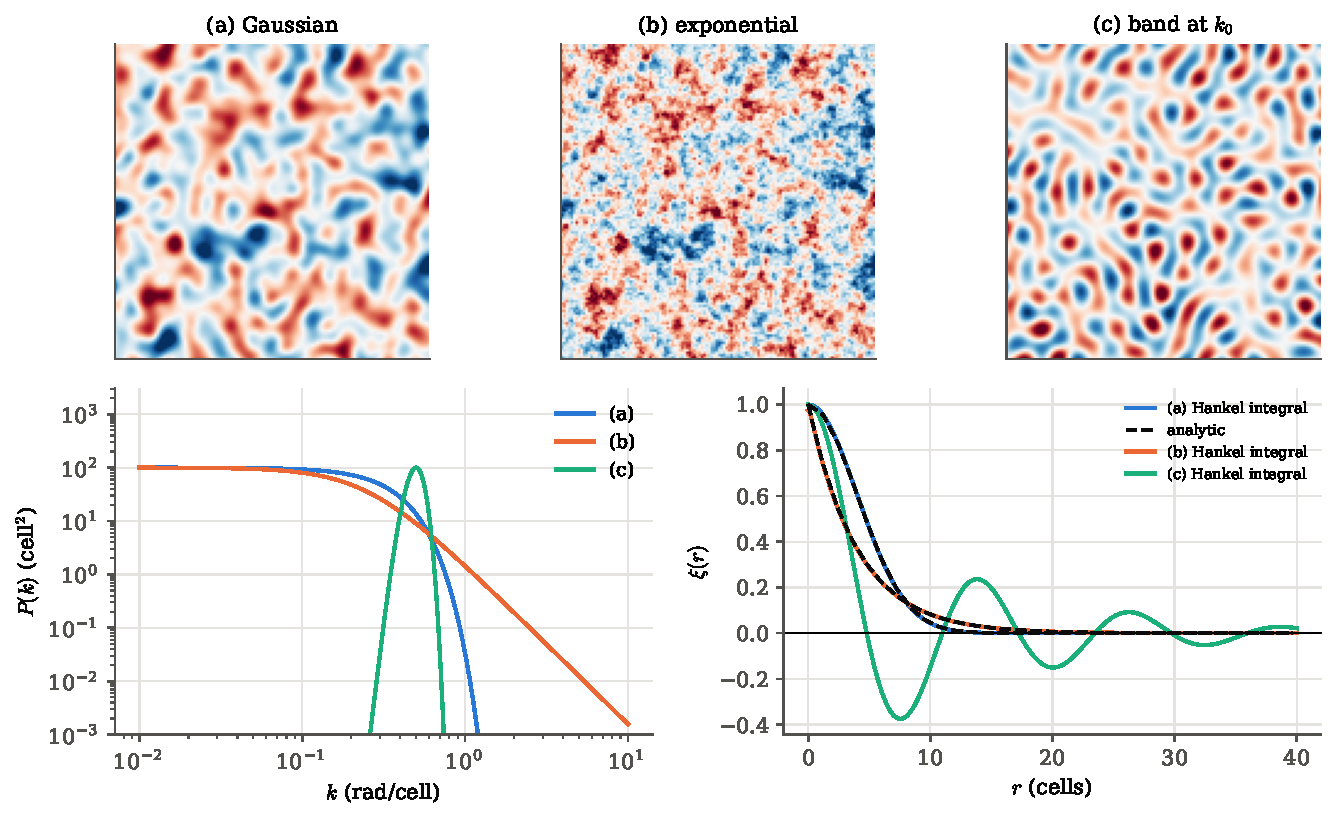
\includegraphics[width=\linewidth]{figures/ch07/pk_xi_pairs.pdf}
\caption{Three spectra coloured onto the same white noise. Top: (a) the Gaussian
pair, smooth blobs of one size; (b) the exponential, whose $k^{-3}$ tail adds
structure on every small scale; (c) a narrow band of wavenumbers, which makes a
cellular pattern. Bottom: the spectra and their correlation functions; the
analytic $\xi$ (dashed) lies on the numerical Hankel transform, and the band
spectrum gives an oscillating $\xi$ with a negative first lobe.}
\label{7a:fig:pk-xi}
\end{figure}

\subsection{A Gaussian field in Fourier space}
\label{7a:sec:grf-fourier}

\emph{Different modes.} For a Gaussian field each $\delta_{\bm k}$ is a linear
combination of Gaussian variables, so the Fourier modes are jointly Gaussian too.
Jointly Gaussian variables that are uncorrelated are independent, so different
modes are independent.

\emph{Inside one mode.} Each $\delta_{\bm k}=a+ib$ is complex, so we also ask
about its real part $a$ and imaginary part $b$. Two facts fix them. First, the
variance of the mode is $\langle|\delta_{\bm k}|^2\rangle=\langle a^2\rangle+\langle b^2\rangle$,
proportional to $P(k)$. Second, for $\bm k\neq\bm 0$ (so that $\bm k\neq-\bm k$)
the reality condition gives
$\langle\delta_{\bm k}\delta_{\bm k}\rangle=\langle\delta_{\bm k}\delta_{-\bm k}^*\rangle$.
That is the covariance of two \emph{different} modes, $\bm k$ and $-\bm k$, so it
vanishes by \eqref{7a:eq:wk}. Writing it out,
\begin{equation*}
  0=\langle(a+ib)^2\rangle=\langle a^2\rangle-\langle b^2\rangle+2i\langle ab\rangle .
\end{equation*}
The real part says $\langle a^2\rangle=\langle b^2\rangle$; the imaginary part says
$\langle ab\rangle=0$. So $a$ and $b$ are independent Gaussians with equal
variance, each carrying half of the mode's power.

\emph{Amplitude and phase.} Then $|\delta_{\bm k}|^2=a^2+b^2$ is a sum of two
squared Gaussians, a scaled $\chi^2_2$, which is an exponential distribution. In
polar form, $\delta_{\bm k}=|\delta_{\bm k}|e^{i\varphi_{\bm k}}$, the amplitude
has the Rayleigh distribution and the phase $\varphi_{\bm k}$ is uniform on
$[0,2\pi)$, independent of the amplitude. This is the same polar decomposition of
two independent Gaussians that gives the Box--Muller method (\cref{ch:06}).

\emph{What it means.} A homogeneous Gaussian field is nothing but a sum of plane
waves with independent Rayleigh amplitudes, whose mean square is set by $P(k)$,
and independent, uniformly random phases. The random amplitudes are why a
measured power spectrum scatters about the true one (\cref{7a:sec:ergodic}). The
random phases are exactly what $P(k)$ ignores (\cref{7a:sec:phases}).
\section{Simulating a Gaussian random field with the FFT}
\label{7a:sec:simulate}

Every later chapter needs fake universes: hundreds of CMB skies to calibrate an
estimator in \cref{ch:08}, mock maps to test a sampler in \cref{ch:09}, Gaussian
fields as the null hypothesis for the topological summaries of \cref{ch:12}.
\emph{The old way.} The Cholesky factor of \cref{ch:06} makes a correlated
Gaussian vector by colouring white noise: $\bm\delta=\mathbf L\bm z$, with
$\bm z$ independent standard normals and $\mathbf L\mathbf L\T=\Cmat$. But it
costs $n^3/3$ operations for $n$ pixels, so it stops at a few thousand pixels.
\emph{The way out.} In the Fourier basis the covariance of a homogeneous field is
diagonal (\cref{7a:sec:fourier}), so its ``Cholesky factor'' is diagonal too:
multiply each Fourier mode of white noise by $\sqrt{P(k)}$. The fast Fourier
transform does the change of basis in about $n\log n$ operations.

\paragraph{The question.} Given a power spectrum $P(k)\ge0$, how do we produce,
on a grid, a real Gaussian field whose Fourier modes have exactly the variance
$P(k)$, and with which normalisation?

\subsection{The box and the grid}
\label{7a:sec:box}

A computer holds a field on a finite grid, and the FFT treats the grid as
periodic. So we work in a cubic box of side $L$ in $d$ dimensions, of volume
$V=L^d$, with periodic boundary conditions. The box is divided into $N$ cells per
side, each of size $\Delta=L/N$; there are $N^d$ cells in all, with centres
$\bm x_{\bm n}=\bm n\Delta$ for an integer vector $\bm n$.

The box and the grid each limit which waves exist. Periodicity allows only the
wavevectors $\bm k=\frac{2\pi}{L}\bm m$ with integer $\bm m$, so there is one
allowed $\bm k$ per cell of volume $(2\pi/L)^d$ in $\bm k$-space. The grid allows
only $|k_a|\le\pi/\Delta$ along each axis $a$. The two ends of that range have
names. The \newterm{fundamental mode} $k_f=2\pi/L$ is the longest wave that fits
in the box. The \newterm{Nyquist wavenumber} $k_{\rm Ny}=\pi N/L$ is the shortest
wave the grid can represent, one that alternates sign from cell to cell. In a
finite box the Fourier series replaces the Fourier integral \eqref{7a:eq:ft}:
\begin{equation}
  \delta_{\bm k}=\int_V\dd^dx\;\delta(\bm x)\,e^{-i\bm k\cdot\bm x},
  \qquad
  \delta(\bm x)=\frac1V\sum_{\bm k}\delta_{\bm k}\,e^{i\bm k\cdot\bm x},
  \label{7a:eq:box-ft}
\end{equation}
and the calculation \eqref{7a:eq:wk} goes through with one change: the $\bm y$
integral over the box gives $\int_V\dd^dy\,e^{-i(\bm k-\bm k')\cdot\bm y}=V\delta_{\bm k\bm k'}$
(the integral of a whole number of periods of a wave vanishes). Hence
\begin{equation}
  \langle\delta_{\bm k}\,\delta_{\bm k'}^*\rangle=V\,P(k)\,\delta_{\bm k\bm k'} .
  \label{7a:eq:box-wk}
\end{equation}
The Dirac delta $(2\pi)^d\delta_D(\bm k-\bm k')$ of the infinite volume has become
the Kronecker delta times the volume, which is how one should read
``$(2\pi)^d\delta_D(\bm 0)=V$''. Every mode has variance $VP(k)$; a bigger box
has more modes, each of larger variance, and the variance per unit volume is the
same.

On the grid the integral in \eqref{7a:eq:box-ft} becomes a sum over cells,
$\delta_{\bm k}\approx\Delta^d\sum_{\bm n}\delta_{\bm n}e^{-i\bm k\cdot\bm x_{\bm n}}=\Delta^dF_{\bm k}$,
where $F_{\bm k}$ is exactly what \pyname{numpy.fft.fftn} returns. The inverse is
exact: $\delta_{\bm n}=\frac1V\sum_{\bm k}\Delta^dF_{\bm k}e^{i\bm k\cdot\bm x_{\bm n}}
=\frac{1}{N^d}\sum_{\bm k}F_{\bm k}e^{i\bm k\cdot\bm x_{\bm n}}$, which is
\pyname{numpy.fft.ifftn}, because $V/\Delta^d=N^d$. Since
$F_{\bm k}=\delta_{\bm k}/\Delta^d$, the target \eqref{7a:eq:box-wk} in numpy's
units is
\begin{equation}
  \langle|F_{\bm k}|^2\rangle=\frac{V\,P(k)}{\Delta^{2d}}=\frac{N^d\,P(k)}{\Delta^d}.
  \label{7a:eq:fft-target}
\end{equation}

\subsection{The recipe, and why it is right}
\label{7a:sec:recipe}

\begin{figure}[htbp]
\centering
\begin{tikzpicture}[
  node distance=4mm,
  blk/.style={draw=accent,thick,rounded corners=2pt,fill=ideabg,
              align=center,font=\small,minimum height=12mm,text width=24mm},
  flow/.style={->,thick,accent}]
  \node[blk] (w) {white noise\\ $w_{\bm n}\iid\Normal(0,1)$\\ one per cell};
  \node[blk,right=of w] (W) {FFT:\\ $W_{\bm k}$, all modes\\ variance $N^d$};
  \node[blk,right=of W] (F) {colour:\\ $F_{\bm k}=W_{\bm k}\sqrt{P(k)/\Delta^d}$};
  \node[blk,right=of F] (d) {inverse FFT:\\ $\delta_{\bm n}$, real,\\ spectrum $P(k)$};
  \draw[flow] (w) -- (W);
  \draw[flow] (W) -- (F);
  \draw[flow] (F) -- (d);
\end{tikzpicture}
\caption{The FFT recipe for a Gaussian random field. White noise has the same
variance in every Fourier mode; multiplying each mode by the square root of the
desired power spectrum, and transforming back, gives a field whose modes have
exactly that variance. It is the Cholesky construction of \cref{ch:06} carried
out in the basis where the covariance is diagonal.}
\label{7a:fig:recipe}
\end{figure}

The recipe has four steps (\cref{7a:fig:recipe}). Draw one independent standard
normal $w_{\bm n}$ per cell. Fourier transform it, $W_{\bm k}=\sum_{\bm n}w_{\bm n}e^{-i\bm k\cdot\bm x_{\bm n}}$.
Multiply each mode by $\sqrt{P(k)/\Delta^d}$. Transform back. To see that the
result has the right covariance, first compute the covariance of the transformed
white noise:
\begin{align}
  \langle W_{\bm k}W_{\bm k'}^*\rangle
  &\eqby{1}\sum_{\bm n}\sum_{\bm m}\langle w_{\bm n}w_{\bm m}\rangle\,
     e^{-i\bm k\cdot\bm x_{\bm n}+i\bm k'\cdot\bm x_{\bm m}}
   \eqby{2}\sum_{\bm n}e^{-i(\bm k-\bm k')\cdot\bm x_{\bm n}}
   \eqby{3}N^d\,\delta_{\bm k\bm k'} .
  \label{7a:eq:white}
\end{align}
\begin{explain}
  \item Definition of $W_{\bm k}$ and of its complex conjugate; average inside the sums.
  \item The noise is independent with unit variance, $\langle w_{\bm n}w_{\bm m}\rangle=\delta_{\bm n\bm m}$,
        which kills one sum.
  \item For $\bm k=\bm k'$ each of the $N^d$ terms is $1$. For $\bm k\neq\bm k'$ the
        terms are the $N$-th roots of unity along at least one axis, which sum to
        zero.
\end{explain}
White noise is a field with the same variance, $N^d$, in every mode and no
correlation between modes: a flat power spectrum, which is where the name comes
from. The colouring then gives, for $F_{\bm k}=W_{\bm k}\sqrt{P(k)/\Delta^d}$,
\begin{equation*}
  \langle F_{\bm k}F_{\bm k'}^*\rangle
  =\sqrt{\tfrac{P(k)}{\Delta^d}}\sqrt{\tfrac{P(k')}{\Delta^d}}\,\langle W_{\bm k}W_{\bm k'}^*\rangle
  =\frac{N^dP(k)}{\Delta^d}\,\delta_{\bm k\bm k'},
\end{equation*}
which is the target \eqref{7a:eq:fft-target}. Three more checks complete the
argument.
\emph{The output is Gaussian,} because it is a linear function of the Gaussian
vector $\bm w$.
\emph{It is real.} The noise $w$ is real, so $W_{-\bm k}=W_{\bm k}^*$.
Multiplying by $\sqrt{P(|\bm k|)}$, which is real and the same at $\bm k$ and
$-\bm k$, keeps $F_{-\bm k}=F_{\bm k}^*$. That is the reality condition
\eqref{7a:eq:reality}, so the inverse transform has no imaginary part.
\emph{Its variance is right.} By Parseval,
\begin{equation}
  \sigma^2=\langle\delta_{\bm n}^2\rangle=\frac{1}{V^2}\sum_{\bm k}\langle|\delta_{\bm k}|^2\rangle
  =\frac1V\sum_{\bm k}P(k)\;\approx\;\int\frac{\dd^dk}{(2\pi)^d}P(k),
  \label{7a:eq:box-sigma}
\end{equation}
the box version of \eqref{7a:eq:sigma2}: the allowed $\bm k$ have density
$V/(2\pi)^d$, so $\frac1V\sum_{\bm k}$ becomes $\int\dd^dk/(2\pi)^d$. Finally, the
$\bm k=0$ mode is the mean of the box. We set it to zero, so every simulated box
has mean exactly zero.

\begin{keyidea}[Colouring white noise in Fourier space]
To simulate a homogeneous Gaussian field with power spectrum $P(k)$ on a periodic
grid: FFT a map of independent standard normals, multiply mode $\bm k$ by
$\sqrt{P(k)/\Delta^d}$, inverse FFT. The cost is $O(N^d\log N^d)$ instead of the
$O(N^{3d})$ of a Cholesky factorisation, and the result is exact for the
band of wavevectors $k_f\le|k_a|\le k_{\rm Ny}$ that the box and the grid can hold.
\end{keyidea}

The implementation in the shared library is ten lines.

\pyfile[firstline=52,lastline=61,firstnumber=52]{code/ch07/lib_fields.py}{The FFT
simulator of a Gaussian random field}

Line 53 is the cell size $\Delta$, line 54 the grid of $|\bm k|$ in the layout of
\pyname{rfftn}, which stores only the half of $\bm k$-space with $k_d\ge0$ because
the other half is fixed by the reality condition. Line 56 is the colouring factor
$\sqrt{P(k)/\Delta^d}$, set to zero at $\bm k=0$. Lines 59--61 are the recipe: white
noise, its FFT, colour, transform back. When \pyname{nsim} is given, the first axis
counts realisations and the transforms act on the remaining $d$ axes, so a stack of
independent fields costs one call. The library also contains the two estimators we
use to check the output, and the sphere version of the same recipe.

\paragraph{Estimating $P(k)$ and $\xi(r)$ from a map.}
Each mode has $\langle|\delta_{\bm k}|^2\rangle=VP(k)$ by \eqref{7a:eq:box-wk}, so
$|\delta_{\bm k}|^2/V$ is a one-mode estimate of $P$. The natural estimate of the
power at wavenumber $k$ averages it over the $N_{\rm modes}$ modes in a thin shell
$k-\frac{\Delta k}{2}<|\bm k|\le k+\frac{\Delta k}{2}$,
\begin{equation}
  \hat P(k)=\frac{1}{N_{\rm modes}}\sum_{\bm k\in\text{shell}}\frac{|\delta_{\bm k}|^2}{V},
  \qquad
  \langle\hat P(k)\rangle=\frac{1}{N_{\rm modes}}\sum_{\bm k\in\text{shell}}P(|\bm k|),
  \label{7a:eq:phat}
\end{equation}
so $\hat P$ is unbiased for the average of $P$ over the shell. The correlation
function could be estimated directly, by averaging $\delta_{\bm n}\delta_{\bm n+\bm r}$
over all cells, but that costs $N^d$ operations for each separation $\bm r$. The
Fourier route is faster: it is the discrete form of Wiener--Khinchin. With
$\delta_{\bm n}$ real,
\begin{align}
  \hat\xi(\bm r)\equiv\frac{1}{N^d}\sum_{\bm n}\delta_{\bm n}\delta_{\bm n+\bm r}
  &\eqby{1}\frac{1}{N^d}\sum_{\bm n}\frac{1}{N^{2d}}\sum_{\bm k,\bm k'}F_{\bm k}^*F_{\bm k'}\,
    e^{-i\bm k\cdot\bm x_{\bm n}+i\bm k'\cdot(\bm x_{\bm n}+\bm r)}
   \nonumber\\
  &\eqby{2}\frac{1}{N^{2d}}\sum_{\bm k}|F_{\bm k}|^2e^{i\bm k\cdot\bm r}
   \eqby{3}\frac{1}{N^d}\,\mathrm{IFFT}\bigl(|F|^2\bigr)(\bm r),
  \label{7a:eq:xihat}
\end{align}
\begin{explain}
  \item Write $\delta_{\bm n}=\delta_{\bm n}^*$ with the inverse FFT, and
        $\delta_{\bm n+\bm r}$ with the inverse FFT.
  \item The sum over cells of $e^{i(\bm k'-\bm k)\cdot\bm x_{\bm n}}$ is $N^d\delta_{\bm k\bm k'}$,
        as in \eqref{7a:eq:white}.
  \item The remaining sum is $N^d$ times the inverse FFT of $|F_{\bm k}|^2$.
\end{explain}
Its expectation, by \eqref{7a:eq:fft-target}, is
$\langle\hat\xi(\bm r)\rangle=\frac1V\sum_{\bm k}P(k)e^{i\bm k\cdot\bm r}\equiv\xi_{\rm box}(\bm r)$:
the correlation function of the field the box can actually hold, periodic, with
no power below $k_f$ or above $k_{\rm Ny}$. It equals the continuum $\xi(r)$ only
for $r\ll L$ and only if $P$ is negligible outside that band. Averaging
\eqref{7a:eq:xihat} over shells of $|\bm r|$ gives the isotropic $\hat\xi(r)$.

\subsection{Two dimensions: power laws}
\label{7a:sec:sim2d}

The script \pyname{code/ch07/05_simulate_2d.py} colours one white-noise map of
$512\times512$ unit cells with the power laws $P=Ak^n$, $n=-1,-2,-3$, choosing $A$
so that \eqref{7a:eq:box-sigma} gives $\sigma^2=1$ in every case
(\cref{7a:fig:simulate-2d}). The look of the maps is set by the slope. For $n=-1$
most of the variance is at small scales and the map looks like noise; for $n=-3$,
where $\Delta^2=k^2P/2\pi\propto k^{-1}$ grows towards large scales, a few
box-sized waves dominate. In each case the measured $\hat P(k)$ follows the input,
and averaged over all shells and $20$ independent maps the ratio
$\hat P/\langle\hat P\rangle$ is $\SevARatioOne$, $\SevARatioTwo$ and $\SevARatioThree$.
The measured $\hat\xi(r)$ of the single map scatters about $\xi_{\rm box}$, and
how far it can stray depends on the slope. In this map the variance $\hat\xi(0)$
is $\SevAXiZeroOne$, $\SevAXiZeroTwo$ and $\SevAXiZeroThree$ for $n=-1,-2,-3$,
although each was designed to be $1$ on average. The $20$ independent maps show
how large such strays are: from map to map $\hat\xi(0)$ scatters by
$\SevAXiZeroSdOne$, $\SevAXiZeroSdTwo$ and $\SevAXiZeroSdThree$. Nothing is wrong
with the simulation. When the variance lives in the few longest waves, one box
contains only a handful of those waves, so it holds only a handful of independent
pieces of information about the variance, and the measured variance scatters
accordingly. \Cref{7a:sec:ergodic} makes this precise.

\begin{figure}[htbp]
\centering
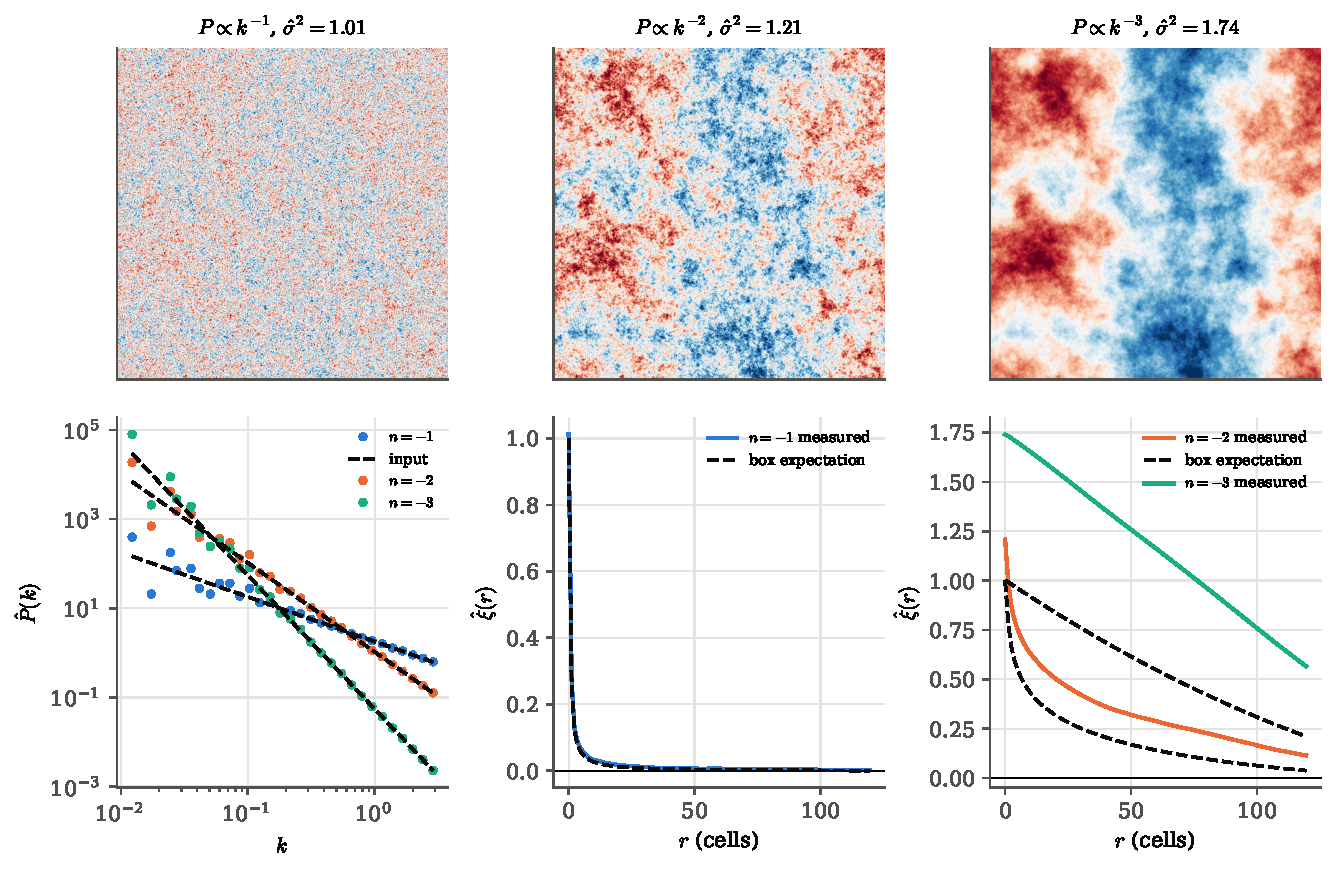
\includegraphics[width=\linewidth]{figures/ch07/simulate_2d.pdf}
\caption{Gaussian fields with power-law spectra $P\propto k^n$, coloured from the
same white noise. Top: $n=-1$, $-2$, $-3$; the steeper the spectrum, the larger the
dominant structures. Bottom left: the shell-averaged power of each map (dots)
against the input averaged over the same modes (dashed). Bottom middle and right:
the measured correlation functions of these maps against their exact box
expectations.}
\label{7a:fig:simulate-2d}
\end{figure}

\subsection{Three dimensions: the matter field and the BAO bump}
\label{7a:sec:sim3d}

The script \pyname{code/ch07/06_simulate_3d_bao.py} takes the linear matter power
spectrum of the fiducial Planck 2018 model at $z=0$ from CAMB (the spectrum of
\cref{ch:T1}, in $(h^{-1}\mathrm{Mpc})^3$) and fills $\SevANsim$ periodic boxes of
side $L=\SevABox\,h^{-1}$Mpc with $\SevANcell^3$ cells of
$\SevACell\,h^{-1}$Mpc. The box holds the wavenumbers from
$k_f=\SevAKf$ to $k_{\rm Ny}=\SevAKNy\,h\,\mathrm{Mpc}^{-1}$, which covers the
turnover of $P(k)$ and the baryon acoustic oscillations. The measured spectra lie on
CAMB's, with a mean ratio $\SevARatioAll$ over the shells and visibly larger
scatter in the first shells, which contain only $\SevANmodesLow$ modes each
(\cref{7a:fig:simulate-3d}). In $r^2\hat\xi(r)$ every box shows the acoustic bump,
which the continuum transform \eqref{7a:eq:xi3d} puts at
$r=\SevARPeak\,h^{-1}$Mpc; the four boxes scatter about the theory by about
$\SevAXiScatter\,(h^{-1}\mathrm{Mpc})^2$ in $r^2\xi$, against a bump height of order
ten. A box of $8\,(h^{-1}\mathrm{Gpc})^3$ is larger than any survey yet completed,
and a real survey also has a mask, noise and galaxies that are biased tracers of
the matter; all of that makes the real measurement harder (\cref{ch:08}).

\begin{figure}[htbp]
\centering
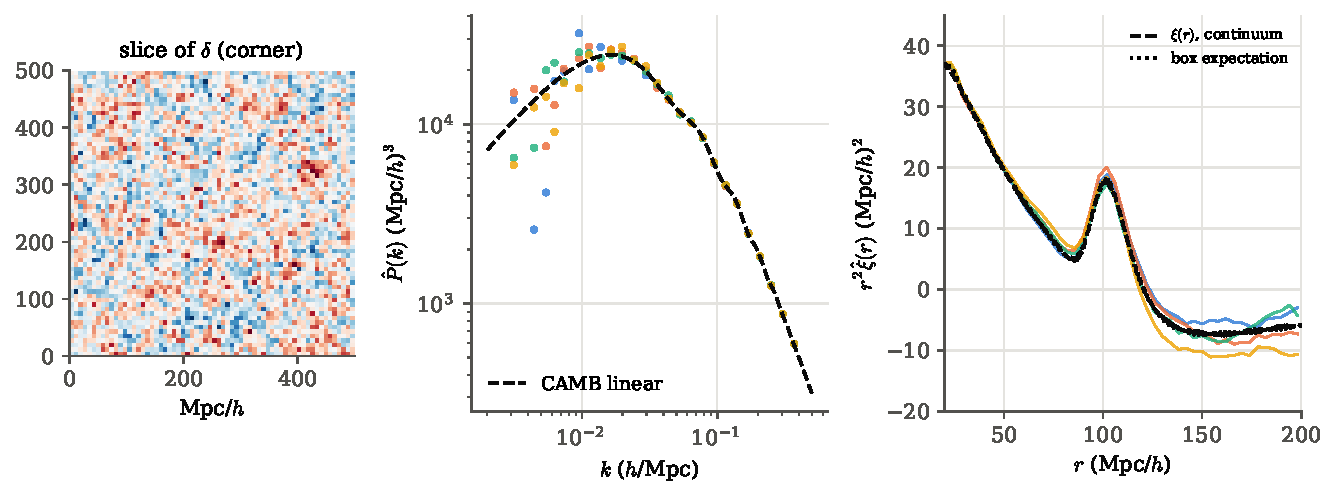
\includegraphics[width=\linewidth]{figures/ch07/simulate_3d_bao.pdf}
\caption{A Gaussian matter field with the linear CAMB spectrum. Left: a
$500\,h^{-1}$Mpc corner of one slice. Middle: the shell-averaged power of four
independent boxes against the input spectrum; the scatter is largest at small $k$,
where shells contain few modes. Right: $r^2\hat\xi(r)$ of the four boxes, the
continuum prediction (dashed) and the exact box expectation (dotted); the acoustic
bump near $100\,h^{-1}$Mpc is recovered in every box.}
\label{7a:fig:simulate-3d}
\end{figure}

\begin{pitfall}[A Gaussian density field can go below $-1$]
The cell-to-cell standard deviation of the simulated matter field is
$\SevASigCell$, so a sizeable fraction of cells have $\delta<-1$, a negative
density. The Gaussian model is a statement about the statistics of the linear
field on large scales, not a model of the density in $8\,h^{-1}$Mpc cells today.
Mock catalogues that must be positive use, for example, a lognormal
transformation of a Gaussian field, which is non-Gaussian
(\cref{7a:fig:gaussian-checks}) and, for the same $P(k)$, has different
higher-order statistics.
\end{pitfall}

\paragraph{The sphere.}
On the sky the plane waves are replaced by spherical harmonics and the Fourier
coefficients by $\alm$, which are independent with variance $\Cell$ for a
statistically isotropic Gaussian field \srcref{HobsonBMC}{(10.2)--(10.3)}. The
library function \pyname{gaussian_field_sphere} applies the same recipe: one
Gaussian per $(\ell,m)$, scaled by $\sqrt{\Cell}$, followed by a spherical-harmonic
transform on a HEALPix grid \cite{Gorski2005}, using our own reproducible random
stream. The full-sky estimator $\Chat$ and its cosmic variance, the sphere's
version of the scatter just seen in the first $k$-shells, are derived for the CMB
in the second half of \cref{ch:07}.
\section{One universe: ergodicity and sample variance}
\label{7a:sec:ergodic}

Every definition so far is an average down the stack of universes of
\cref{7a:fig:ensemble}: $\xi(r)$ is the ensemble average of
$\delta(\bm x)\delta(\bm x+\bm r)$ at fixed points, $P(k)$ the ensemble variance of
a mode. But we have one universe. What we can actually compute is an average
\emph{across} our one map: for example the volume average
$\hat\xi(r)=\frac1V\int_V\dd^dx\,\delta(\bm x)\delta(\bm x+\bm r)$ over a region
of volume $V$, or the shell average $\hat P(k)$ of \eqref{7a:eq:phat}. Using the
second kind of average in place of the first is the \newterm{ergodic
hypothesis}. It is an assumption about the field, it can fail, and even when it
holds it leaves a finite-volume error that no instrument can remove.

\paragraph{The questions.} (1) When does an average over one large volume
converge to the ensemble average? (2) For a finite volume, how far from the
ensemble value is the spatial average likely to be, for the mean and for the
power spectrum?

\subsection{The variance of a spatial average}
\label{7a:sec:var-mean}

Start with the simplest spatial average, the mean of the field over a region of
volume $V$, $\bar\delta_V=\frac1V\int_V\dd^dx\,\delta(\bm x)$. Its ensemble mean is
the ensemble mean of the field, which is zero. The question is how much it
scatters from one universe to the next, that is, its variance:
\begin{align}
  \Var\bar\delta_V
  &\eqby{1}\frac{1}{V^2}\int_V\dd^dx\int_V\dd^dy\;\langle\delta(\bm x)\delta(\bm y)\rangle
   \eqby{2}\frac{1}{V^2}\int_V\dd^dx\int_V\dd^dy\;\xi(\bm x-\bm y)
   \nonumber\\
  &\relby{3}{\approx}\frac{1}{V^2}\int_V\dd^dx\int\dd^dr\;\xi(\bm r)
   \eqby{4}\frac1V\int\dd^dr\;\xi(\bm r)
   \eqby{5}\frac{P(0)}{V} .
  \label{7a:eq:var-mean}
\end{align}
\begin{explain}
  \item Square the average and take the expectation inside both integrals; it is
        the continuum version of the variance of a sum, a double sum of
        covariances \mainref{p.~53, Thm.~3.20}.
  \item Homogeneity, \eqref{7a:eq:homog}.
  \item For fixed $\bm x$, substitute $\bm r=\bm y-\bm x$. If the region is much
        larger than the range of $\xi$, then for almost every $\bm x$ all the
        separations where $\xi$ is non-negligible keep $\bm y$ inside the region,
        and the $\bm r$ integral may be extended over all space. Only a shell of
        thickness about one correlation length at the edge violates this.
  \item The $\bm r$ integral no longer depends on $\bm x$, and $\int_V\dd^dx=V$.
  \item By \eqref{7a:eq:wk} at $\bm k=0$, $P(0)=\int\dd^dr\,\xi(\bm r)$.
\end{explain}
\emph{What it means.} A correlated field over a volume $V$ is worth as much as a
certain number of independent measurements, one per \emph{correlation volume}.
To see this, recall that the mean of $n$ independent measurements of variance
$\sigma^2$ has variance $\sigma^2/n$ (\cref{ch:03}), and write
\eqref{7a:eq:var-mean} in the same form:
\begin{equation}
  \Var\bar\delta_V\approx\frac{\sigma^2}{N_{\rm eff}},
  \qquad
  N_{\rm eff}=\frac{V}{V_c},
  \qquad
  V_c\equiv\frac{1}{\sigma^2}\int\dd^dr\,\xi(r) .
  \label{7a:eq:neff}
\end{equation}
The volume $V$ acts like $N_{\rm eff}$ independent measurements, one per
correlation volume $V_c$, because neighbouring points repeat each other's
information. In words: a survey of volume $V$ contains about $V/L^3$
statistically independent patches of size $L$, and the scatter between surveys
that this causes is called cosmic variance.

\paragraph{When the average converges: ergodicity.}
Equation \eqref{7a:eq:var-mean} answers question (1) for the mean. The spatial
average converges to the ensemble mean, in the sense that its variance goes to
zero, whenever $\frac{1}{V^2}\int_V\int_V\xi\to0$ as $V\to\infty$. It is enough
that $\xi(r)\to0$ as $r\to\infty$: then $\int_V\xi$ grows more slowly than $V$,
and dividing by $V^2$ sends the variance to zero. A field for which spatial
averages converge to ensemble averages is called \newterm{ergodic}.

For estimating $\xi$ itself, the same argument applies with the field replaced by
the products $\delta(\bm x)\delta(\bm x+\bm r)$. It now needs the covariance of
two such products, a four-point function, to die away at large distances. For a
Gaussian field Wick's theorem \eqref{7a:eq:wick} writes that four-point function
as products of $\xi$'s, so a correlation function that decays fast enough makes
$\hat\xi$ converge as well \cite{Peacock1999}.

\paragraph{Example: a field that is not ergodic.}
Add to a Gaussian field $g(\bm x)$ a constant $A\sim\Normal(0,\sigma_A^2)$, drawn
once per universe and the same at every point: $\delta(\bm x)=A+g(\bm x)$. The
result is homogeneous, isotropic and Gaussian, with
$\xi_\delta(r)=\sigma_A^2+\xi_g(r)$. But $\xi_\delta\to\sigma_A^2\neq0$ at large $r$,
and \eqref{7a:eq:var-mean} becomes
$\Var\bar\delta_V\to\sigma_A^2+P_g(0)/V\to\sigma_A^2$. However large the volume,
the spatial mean converges to $A$, the offset of \emph{our} universe, and never to
the ensemble mean $0$. This is not a mathematical curiosity. To a survey,
fluctuation modes with wavelengths longer than the survey are exactly such an
offset: they shift its mean density, and no measurement inside the survey can
tell them apart from a different background.

\paragraph{Checking it on simulated maps.}
The script \pyname{code/ch07/07_sample_variance.py} draws $200$ maps of
$256\times256$ cells with the Gaussian $\xi=e^{-r^2/2\ell^2}$, $\ell=4$, cuts each
into square patches of side $s$, and measures the variance of the patch means
(\cref{7a:fig:sample-variance}, right). For this field
$P(0)=2\pi\ell^2=\SevAPZero$ cells$^2$, so the correlation area is about $100$ cells.
At $s=64$ the measured variance is $\SevAVarSixtyFour\pm\SevAVarSixtyFourErr$ (the
error from the scatter between the $200$ independent maps), the exact expression on the
first line of \eqref{7a:eq:var-mean}, evaluated with the box modes, gives
$\SevAThSixtyFour$, and the large-patch limit $P(0)/s^2$ gives
$\SevAAsySixtyFour$. The limit overestimates slightly because it ignores the edge
shell of step (3), where pairs straddling the boundary are lost. With the extra
offset of standard deviation $\SevASigA$ the variance at $s=64$ is
$\SevANonSixtyFour$, and it flattens at $\sigma_A^2=0.25$ instead of falling: the
non-ergodic field never averages down.

\begin{pitfall}[Ergodicity is an assumption about the ensemble]
No test on one realisation can prove that a field is ergodic, because the
non-ergodic part (the offset $A$ above, or modes larger than the survey) looks
like a constant in every map. Ergodicity is part of the model, justified by the
physics (here, by the decay of $\xi$ predicted by the theory), and its failure on
the largest scales is one reason those scales are the hardest to measure.
\end{pitfall}

\subsection{The sample variance of the power spectrum}
\label{7a:sec:sample-var}

The power spectrum is estimated from one map by averaging $|\delta_{\bm k}|^2/V$
over a shell of wavevectors, \eqref{7a:eq:phat}. \emph{The question.} How far
from $P(k)$ is that average likely to be? For a Gaussian field the answer is
exact, because we know the distribution of every mode
(\cref{7a:sec:grf-fourier}). \emph{One mode first.} For a wavevector that is not
its own negative, $\delta_{\bm k}=a+ib$ with $a$ and $b$ independent Gaussians,
each of variance $VP/2$ (half of the mode variance $VP$ of \eqref{7a:eq:box-wk}),
so
\begin{equation}
  x_{\bm k}\equiv\frac{|\delta_{\bm k}|^2}{VP(k)}=\frac{a^2+b^2}{VP}
  \sim\tfrac12\chi^2_2=\text{Exponential}(1),
  \qquad \E x=1,\quad \Var x=1 .
  \label{7a:eq:mode-exp}
\end{equation}
A single mode is a terrible estimate of the power: its standard deviation equals
its mean. \emph{Then the shell.} Averaging helps, but only over
\emph{independent} modes, and here the reality condition matters. The shell
contains $N_{\rm modes}$ wavevectors, but they come in pairs $\pm\bm k$ with
$|\delta_{-\bm k}|^2=|\delta_{\bm k}^*|^2=|\delta_{\bm k}|^2$, so only
$N_{\rm modes}/2$ of the values are independent (\cref{7a:fig:kshell}). Then
\begin{align}
  \Var\hat P
  &\eqby{1}\Var\Bigl(\frac{2}{N_{\rm modes}}\sum_{\text{pairs}}\frac{|\delta_{\bm k}|^2}{V}\Bigr)
   \eqby{2}\frac{4}{N_{\rm modes}^2}\cdot\frac{N_{\rm modes}}{2}\cdot P^2\Var x
   \eqby{3}\frac{2P^2}{N_{\rm modes}} ,
  \label{7a:eq:var-phat}
\end{align}
\begin{explain}
  \item Group the shell sum into $N_{\rm modes}/2$ pairs of equal terms; each pair
        contributes $2|\delta_{\bm k}|^2/V$.
  \item The pairs are independent, so the variance of the sum is the sum of
        $N_{\rm modes}/2$ equal variances, each $\Var(|\delta_{\bm k}|^2/V)=P^2\Var x$
        (we take $P$ constant across the thin shell).
  \item $\Var x=1$ by \eqref{7a:eq:mode-exp}.
\end{explain}

\begin{keyidea}[Sample variance of the power spectrum]
For a Gaussian field measured without noise over a volume $V$, the shell-averaged
power has fractional error
\begin{equation*}
  \frac{\Delta\hat P}{P}=\sqrt{\frac{2}{N_{\rm modes}}},
  \qquad
  N_{\rm modes}=\begin{cases}
     \dfrac{V\,k^2\Delta k}{2\pi^2} & (3\text{D}),\\[8pt]
     \dfrac{A\,k\,\Delta k}{2\pi} & (2\text{D, area }A).
  \end{cases}
\end{equation*}
The ``$2$'' comes from the reality condition: $\pm\bm k$ carry the same
information. In fact $N_{\rm modes}\hat P/P\sim\chi^2_{N_{\rm modes}}$, a sum of
$N_{\rm modes}/2$ independent $\chi^2_2$ variables.
\end{keyidea}

The mode count is density times volume. The allowed wavevectors sit on a lattice
with one point per cell of volume $(2\pi/L)^d$ in $\bm k$-space
(\cref{7a:sec:box}), a density of $V/(2\pi)^d$ points. A thin shell has volume
$4\pi k^2\Delta k$ in 3D and $2\pi k\Delta k$ in 2D. Multiplying gives the two
cases of $N_{\rm modes}$ above. On the sphere
the same counting gives $2\ell+1$ real degrees of freedom at multipole $\ell$, and
the full-sky estimator has $\Var\Chat/\Cell^2=2/(2\ell+1)$, the cosmic variance of
the CMB derived later in \cref{ch:07}.

\begin{figure}[htbp]
\centering
\begin{tikzpicture}[x=0.42cm,y=0.42cm]
  \fill[formblue!10,even odd rule] (0,0) circle (4.5) (0,0) circle (3.5);
  \draw[formblue!60] (0,0) circle (4.5);
  \draw[formblue!60] (0,0) circle (3.5);
  \foreach \i in {-5,...,5}{\foreach \j in {-5,...,5}{
    \pgfmathsetmacro{\rr}{sqrt(\i*\i+\j*\j)}
    \ifdim \rr pt>3.5pt \ifdim \rr pt<4.5pt
      \fill[formblue] (\i,\j) circle (3.2pt);
    \else \fill[softgray!70] (\i,\j) circle (1.6pt); \fi
    \else \fill[softgray!70] (\i,\j) circle (1.6pt); \fi}}
  \fill[bdryred] (4,1) circle (4pt);
  \fill[bdryred] (-4,-1) circle (4pt);
  \node[lbl,bdryred,anchor=west] at (5.4,1) {$\bm k$};
  \node[lbl,bdryred,anchor=east] at (-5.4,-1) {$-\bm k$};
  \draw[faint,->] (-6,0) -- (6.3,0) node[anchor=west,lbl] {$k_x$};
  \draw[faint,->] (0,-6) -- (0,6.3) node[anchor=south,lbl] {$k_y$};
  \node[lbl,align=left,anchor=west] at (7.5,3)
    {lattice spacing $k_f=2\pi/L$\\ shell $3.5k_f<|\bm k|\le4.5k_f$:\\ $N_{\rm modes}=$ blue points\\ independent values $=N_{\rm modes}/2$};
\end{tikzpicture}
\caption{Counting modes in two dimensions. The allowed wavevectors form a square
lattice of spacing $k_f=2\pi/L$. The power at $|\bm k|\approx4k_f$ is estimated
from the blue points in the shell. The red pair $\bm k$, $-\bm k$ carries a single
independent value of $|\delta_{\bm k}|^2$, because $\delta_{-\bm k}=\delta_{\bm k}^*$.}
\label{7a:fig:kshell}
\end{figure}

\paragraph{Checking it.}
\Cref{7a:fig:sample-variance} tests both steps on simulated maps. Over
$\SevAModeCount$ modes of $50$ maps, the normalised power $x_{\bm k}$ has mean
$\SevAModeMean$ and variance $\SevAModeVar$, and its histogram is the exponential
$e^{-x}$ over three decades (left). Over $500$ maps of $128\times128$ cells and $60$
shells, the scatter of $\hat P$ follows $\sqrt{2/N_{\rm modes}}$ (middle): the first
shell, with $\SevANmFirst$ modes, scatters by $\SevAFracFirst$ against
$\sqrt{2/4}=\SevAPredFirst$, the tenth, with $\SevANmTen$ modes, by $\SevAFracTen$
against $\SevAPredTen$, and averaged over all shells the ratio of measured to
predicted scatter is $\SevAFracRatio$. The scatter of the steep-spectrum maps in
\cref{7a:fig:simulate-2d} and of the first $k$-shells in
\cref{7a:fig:simulate-3d} is this effect: there, most of the variance sat in
shells with a handful of modes.

\begin{figure}[htbp]
\centering
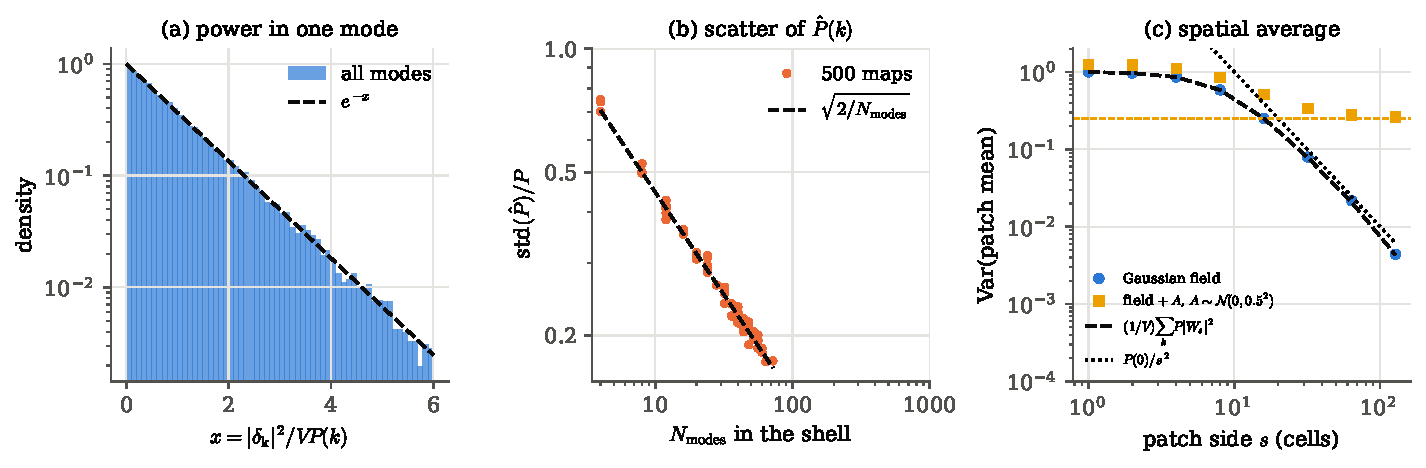
\includegraphics[width=\linewidth]{figures/ch07/sample_variance.pdf}
\caption{One universe, finite volume. Left: the power in a single Fourier mode,
in units of its expectation, is exponentially distributed (log scale). Middle:
the fractional scatter of the shell-averaged $\hat P(k)$ over $500$ maps falls as
$\sqrt{2/N_{\rm modes}}$. Right: the variance of the mean over an $s\times s$ patch
falls as $P(0)/s^2$ for the Gaussian field (blue), following the exact box
prediction (dashed); with a random offset per universe (orange) it stalls at the
offset's variance.}
\label{7a:fig:sample-variance}
\end{figure}

\paragraph{Example: how well can a galaxy survey measure $P(k)$?}
Take an idealised survey of volume $V=1\,(h^{-1}\mathrm{Gpc})^3=10^9\,(h^{-1}\mathrm{Mpc})^3$,
no noise, and shells of width $\Delta k=0.01\,h\,\mathrm{Mpc}^{-1}$ at
$k=0.1\,h\,\mathrm{Mpc}^{-1}$:
\begin{align*}
  N_{\rm modes}=\frac{V\,k^2\Delta k}{2\pi^2}
  =\frac{10^9\times10^{-2}\times10^{-2}}{19.74}=5066,
  \qquad
  \frac{\Delta\hat P}{P}=\sqrt{\frac{2}{5066}}=2.0\% .
\end{align*}
At $k=0.01\,h\,\mathrm{Mpc}^{-1}$ with $\Delta k=0.005\,h\,\mathrm{Mpc}^{-1}$ the same
survey has $N_{\rm modes}=10^9\times10^{-4}\times0.005/19.74=25$ and
$\Delta\hat P/P=28\%$. Large scales are always measured worst, because a fixed
volume holds few long waves. The only remedy is a bigger volume; a better
detector does not help.

\begin{pitfall}[Sample variance is not noise]
The error $\sqrt{2/N_{\rm modes}}$ is present in a perfect, noise-free measurement
of the whole field. It comes from the randomness of the field itself: our
universe is one draw. Instrument noise adds to it (white noise of power $N$
multiplies $\sqrt{2/N_{\rm modes}}$ by $(P+N)/P$), but removing the noise never
removes it.
\end{pitfall}

In a periodic box the $\hat P$ in different shells are uncorrelated; in a real
survey they are not. In the box, different shells contain different modes, and
different modes are independent. A survey does not observe a periodic box. It
multiplies the field by a window (the survey footprint), and multiplication in
real space is convolution in Fourier space. The convolution mixes neighbouring
modes and so correlates the shells \srcref{HobsonBMC}{p.~136, (6.5)}. Undoing that mixing on
the sphere is the pseudo-$\Cell$ problem of \cref{ch:08}.
\section{Smoothing: beams, pixels and window functions}
\label{7a:sec:smoothing}

No instrument records a field at a point. A telescope sees the sky through a beam
a few arcminutes wide; a detector pixel integrates over its area; a galaxy survey
counts galaxies in cells, or spheres, of finite size. Analysts also smooth on
purpose: the amplitude of matter fluctuations is quoted as $\sigma_8$, the
standard deviation of the density averaged over spheres of radius
$8\,h^{-1}$Mpc, and the topological summaries of \cref{ch:12} are always computed
on a field smoothed at a chosen scale. In each case the observed field is a
weighted average of the true field over a neighbourhood. The averaging leaves
the field homogeneous and Gaussian, and its effect on the power spectrum is a
single multiplication.

\begin{workdef}[window function]
A \newterm{window function} $W_R(\bm x)$ is a weight centred on the origin with
characteristic width $R$ and $\int\dd^dx\,W_R(\bm x)=1$. The field
\newterm{smoothed} on scale $R$ is the convolution
\begin{equation}
  \delta_R(\bm x)=\int\dd^dy\;W_R(\bm x-\bm y)\,\delta(\bm y)
  \label{7a:eq:smooth}
\end{equation}
\unpack{the weighted average of $\delta$ around $\bm x$, with weights $W_R$}.
Its Fourier transform $W(\bm k)$ is also called the window function; the
normalisation means $W(\bm 0)=1$.
\emph{Examples:} a Gaussian beam, a top-hat sphere (counts in cells), a square
pixel.
\end{workdef}

\paragraph{The question.} If we know the power spectrum $P(k)$ of the true field,
what are the power spectrum, the correlation function and the variance of the
smoothed field?

\subsection{The convolution theorem does all the work}
\label{7a:sec:convolution}

Fourier transform \eqref{7a:eq:smooth} with the convention \eqref{7a:eq:ft}:
\begin{align}
  \delta_{R,\bm k}
  &\eqby{1}\int\dd^dx\;e^{-i\bm k\cdot\bm x}\int\dd^dy\;W_R(\bm x-\bm y)\,\delta(\bm y)
   \eqby{2}\int\dd^dy\;\delta(\bm y)\,e^{-i\bm k\cdot\bm y}
     \int\dd^du\;W_R(\bm u)\,e^{-i\bm k\cdot\bm u}
   \nonumber\\
  &\eqby{3}W(\bm k)\,\delta_{\bm k} .
  \label{7a:eq:conv}
\end{align}
\begin{explain}
  \item Definitions \eqref{7a:eq:ft} and \eqref{7a:eq:smooth}.
  \item Swap the order of integration and, for fixed $\bm y$, substitute
        $\bm u=\bm x-\bm y$; then $e^{-i\bm k\cdot\bm x}=e^{-i\bm k\cdot\bm y}e^{-i\bm k\cdot\bm u}$
        and the two integrals separate.
  \item Each integral is a Fourier transform.
\end{explain}
Smoothing acts mode by mode: each Fourier mode is multiplied by a number,
$W(\bm k)$. Multiplying each mode by its own number cannot make two different
modes correlated, so the covariance of the smoothed modes follows at once from
\eqref{7a:eq:wk}:
\begin{equation}
  \langle\delta_{R,\bm k}\,\delta_{R,\bm k'}^*\rangle
  =W(\bm k)W^*(\bm k')\langle\delta_{\bm k}\delta_{\bm k'}^*\rangle
  =(2\pi)^d\delta_D(\bm k-\bm k')\,|W(\bm k)|^2P(k).
  \label{7a:eq:pr}
\end{equation}

\begin{keyidea}[Smoothing multiplies the power spectrum by $|W|^2$]
A smoothed homogeneous field is homogeneous, with
\begin{equation*}
  P_R(k)=|W(k)|^2P(k),
  \qquad
  \sigma_R^2=\langle\delta_R^2\rangle=\int\frac{\dd^dk}{(2\pi)^d}\,|W(k)|^2P(k).
\end{equation*}
If the field is Gaussian, so is the smoothed field, since \eqref{7a:eq:smooth} is
linear. Smoothing removes power at $k\gtrsim1/R$ and leaves larger scales alone.
\end{keyidea}

\subsection{The common windows}
\label{7a:sec:windows}

\paragraph{Gaussian.}
$W_R(\bm x)=(2\pi R^2)^{-d/2}e^{-x^2/2R^2}$. Its transform is
\eqref{7a:eq:gauss-pair} divided by the normalising constant $(2\pi R^2)^{d/2}$,
\begin{equation}
  W(k)=e^{-k^2R^2/2} .
  \label{7a:eq:wgauss}
\end{equation}
It is the standard model of a telescope beam; a beam of full width at half
maximum $\theta_{\rm FWHM}$ has $R=\theta_{\rm FWHM}/\sqrt{8\ln2}$.

\paragraph{Top-hat sphere.}
In three dimensions, $W_R(\bm x)=\frac{3}{4\pi R^3}$ for $|\bm x|<R$ and zero
outside: the average over a ball, which is what counting galaxies in spheres
does. It is isotropic, so the 3D radial transform (the inverse of
\eqref{7a:eq:xi3d}) applies:
\begin{align}
  W(k)
  &\eqby{1}\frac{3}{4\pi R^3}\int_0^R4\pi r^2\,\frac{\sin kr}{kr}\,\dd r
   \eqby{2}\frac{3}{R^3k}\Bigl[\frac{\sin kr}{k^2}-\frac{r\cos kr}{k}\Bigr]_0^R
   \eqby{3}\frac{3\,(\sin x-x\cos x)}{x^3},\quad x=kR .
  \label{7a:eq:wtophat}
\end{align}
\begin{explain}
  \item $W(k)=4\pi\int r^2\dd r\,W_R(r)\frac{\sin kr}{kr}$ with the constant weight
        inside the ball.
  \item Cancel $4\pi$ and one power of $r$, and integrate $r\sin kr$ by parts:
        $\int r\sin kr\,\dd r=\frac{\sin kr}{k^2}-\frac{r\cos kr}{k}$.
  \item Evaluate at $r=R$ (the lower limit gives $0$) and write $x=kR$.
\end{explain}
For small $x$, $\sin x-x\cos x=\frac{x^3}{3}-\frac{x^5}{30}+\dots$, so $W\to1$ as it
must. This is the $W$ in the $\sigma_8$ integral,
$\sigma_8^2=\int_0^\infty\frac{k^2\dd k}{2\pi^2}P(k)\,W^2(k\cdot8\,h^{-1}\mathrm{Mpc})$,
evaluated with the CAMB spectrum in \cref{ch:T1}.

\paragraph{Disc.}
In two dimensions the average over a disc of radius $R$ has, by the 2D radial
transform and the identity $\frac{\dd}{\dd x}[xJ_1(x)]=xJ_0(x)$,
\begin{equation}
  W(k)=\frac{1}{\pi R^2}\int_0^R2\pi r\,J_0(kr)\,\dd r=\frac{2}{R^2}\cdot\frac{R\,J_1(kR)}{k}
  =\frac{2J_1(kR)}{kR} .
  \label{7a:eq:wdisc}
\end{equation}

\paragraph{Square patch.}
The patch means of \cref{7a:sec:var-mean} (the field averaged over square
patches of side $s$) are a smoothing too. The average over a square has
$W(\bm k)=\prod_a\frac{\sin(k_as/2)}{k_as/2}$, the product of the transforms of
one-dimensional boxes, one per axis $a$. So the variance of the patch mean is
$\sigma_R^2$ with this window. On the grid of the simulation it is the box sum
$\frac1V\sum_{\bm k}P(k)|W(\bm k)|^2$, which gave the dashed curve of
\cref{7a:fig:sample-variance}. The same formula also explains the large-patch
limit $P(0)/V$ of \eqref{7a:eq:var-mean}. For a large patch, $|W|^2$ is a narrow
spike around $\bm k=0$, of area $(2\pi)^d/V$ with $V=s^d$ the patch volume. Over
so narrow a spike $P$ is nearly constant, equal to $P(0)$, so the integral is
$P(0)\cdot\frac{(2\pi)^d}{V}\cdot\frac{1}{(2\pi)^d}=P(0)/V$.

\begin{figure}[htbp]
\centering
\begin{tikzpicture}
\pgfplotsset{every axis/.append style={width=6.4cm,height=4.6cm,grid=major,
  grid style={softgray!25},tick label style={font=\scriptsize},label style={font=\small},
  legend style={font=\scriptsize,draw=none,fill=none}}}
\begin{axis}[xlabel={$x/R$},ylabel={$W_R(x)\,(4\pi R^3/3)$},xmin=0,xmax=3,ymin=0,ymax=1.2,
  legend pos=north east]
  \addplot[very thick,formblue,domain=0:3,samples=120]
     {(4*pi/3)*exp(-x^2/2)/((2*pi)^1.5)};
  \addlegendentry{Gaussian}
  \addplot[very thick,fibreorange] coordinates {(0,1) (1,1) (1,0) (3,0)};
  \addlegendentry{top-hat}
\end{axis}
\begin{axis}[xshift=7.6cm,xlabel={$kR$},ylabel={$W(k)$},xmin=0,xmax=12,ymin=-0.15,ymax=1.05,
  legend pos=north east]
  \addplot[very thick,formblue,domain=0:12,samples=200] {exp(-x^2/2)};
  \addlegendentry{$e^{-k^2R^2/2}$}
  \addplot[very thick,fibreorange,domain=0:0.5,samples=10,forget plot]
     {1-x^2/10+x^4/280};
  \addplot[very thick,fibreorange,domain=0.5:12,samples=300]
     {3*(sin(deg(x))-x*cos(deg(x)))/x^3};
  \addlegendentry{$3(\sin x-x\cos x)/x^3$}
  \addplot[faint,domain=0:12,forget plot] {0};
\end{axis}
\end{tikzpicture}
\caption{The two standard three-dimensional windows. Left: in real space, the
Gaussian (scaled to the top-hat's height convention) and the top-hat ball of
radius $R$. Right: their Fourier transforms. Both are $1$ at $k=0$ and cut off near
$kR\approx2$; the sharp edge of the top-hat leaves oscillating side lobes that let
through some power at $kR\gg1$, which the Gaussian suppresses completely.}
\label{7a:fig:windows}
\end{figure}

\paragraph{Example: smoothing white noise.}
Pixel noise of variance $\sigma_n^2$ in cells of area $\Delta^2$ has
$\xi=\sigma_n^2\delta_{\bm r,\bm 0}$, so $P(k)=\sum_{\bm r}\Delta^2\xi(\bm r)e^{-i\bm k\cdot\bm r}=\sigma_n^2\Delta^2$,
flat. Smooth it with a 2D Gaussian of width $R\gg\Delta$:
\begin{align}
  \sigma_R^2
  &\eqby{1}\int\frac{\dd^2k}{(2\pi)^2}\,\sigma_n^2\Delta^2\,e^{-k^2R^2}
   \eqby{2}\frac{\sigma_n^2\Delta^2}{2\pi}\int_0^\infty k\,e^{-k^2R^2}\,\dd k
   \eqby{3}\frac{\sigma_n^2\Delta^2}{4\pi R^2} .
  \label{7a:eq:white-smooth}
\end{align}
\begin{explain}
  \item The variance formula for $\sigma_R^2$ with $|W|^2=e^{-k^2R^2}$ from \eqref{7a:eq:wgauss}.
  \item Polar coordinates, $\dd^2k=2\pi k\,\dd k$.
  \item $\int_0^\infty k\,e^{-k^2R^2}\dd k=\frac{1}{2R^2}$.
\end{explain}
The noise variance falls as if we had averaged $4\pi R^2/\Delta^2$ independent
pixels: a Gaussian beam of width $R$ has an effective area $4\pi R^2$. For
$R=2$ pixels the noise r.m.s.\ drops by a factor
$\sqrt{4\pi\cdot2^2}=2\sqrt\pi\times2\approx7.1$. This is the trade-off of every
smoothed map: less noise, less resolution.

\subsection{Gradients and spectral moments}
\label{7a:sec:moments}

The variance is the first of a family. Because $\nabla$ acting on
$e^{i\bm k\cdot\bm x}$ brings down $i\bm k$, the gradient of the smoothed field has
Fourier modes $i\bm k\,\delta_{R,\bm k}$, and by \eqref{7a:eq:pr}
\begin{equation}
  \langle|\nabla\delta_R|^2\rangle=\int\frac{\dd^dk}{(2\pi)^d}\,k^2|W(k)|^2P(k)\equiv\sigma_1^2,
  \qquad
  \sigma_j^2\equiv\int\frac{\dd^dk}{(2\pi)^d}\,k^{2j}|W(k)|^2P(k),
  \label{7a:eq:moments}
\end{equation}
the \newterm{spectral moments} of \cite{BBKS1986}, with $\sigma_0=\sigma_R$.

\emph{What $\sigma_1/\sigma_0$ measures.} The ratio is an inverse length. Its
inverse, $\sigma_0/\sigma_1$, is the typical distance over which the field
changes by its own r.m.s., and so the typical spacing of its hot and cold spots.
\emph{Why it matters.} The expected number of peaks of a Gaussian field, and the
expected Euler characteristic of its excursion sets, depend on the power spectrum
only through such moments \cite{BBKS1986,SchmalzingGorski1998}. Those counts are
the topological summaries of \cref{ch:12}. For a Gaussian field they carry no
information beyond $P(k)$; their value lies in what they reveal when the field is
\emph{not} Gaussian.

Without smoothing, the moments of a power law can diverge. With $P=A/k$ in 2D,
$\sigma_1^2\propto\int k^2\cdot\frac{A}{k}\cdot k\,\dd k$, which grows like
$k_{\rm Ny}^3$ as the upper limit $k_{\rm Ny}$ grows. So the unsmoothed field is
rough on the scale of the pixel, and its count of hot spots is set by the grid,
not by the physics. A Gaussian window cures this:
\begin{align*}
  \sigma_0^2=\frac{A}{2\pi}\int_0^\infty e^{-k^2R^2}\dd k=\frac{A}{2\pi}\frac{\sqrt\pi}{2R},
  \qquad
  \sigma_1^2=\frac{A}{2\pi}\int_0^\infty k^2e^{-k^2R^2}\dd k=\frac{A}{2\pi}\frac{\sqrt\pi}{4R^3},
  \qquad
  \frac{\sigma_1}{\sigma_0}=\frac{1}{\sqrt2\,R},
\end{align*}
using $\int_0^\infty e^{-k^2R^2}\dd k=\frac{\sqrt\pi}{2R}$ and
$\int_0^\infty k^2e^{-k^2R^2}\dd k=\frac{\sqrt\pi}{4R^3}$. Every count of features
in a smoothed map must therefore say on which scale $R$ it was smoothed.

\paragraph{Checking it.}
The script \pyname{code/ch07/08_smoothing.py} smooths one $512\times512$ map with
$P=A/k$ and unit raw variance by Gaussian and disc windows
(\cref{7a:fig:smoothing}). The smoothed power spectra lie on $|W|^2P$, including the
side lobes of the disc's $J_1$. At $R=4$ cells the Gaussian-smoothed map has
$\sigma_R=\SevASigRFourG$ against the predicted $\SevASigRFourThG$, the
disc-smoothed one $\SevASigRFourD$ against $\SevASigRFourThD$; the disc keeps more
variance because it averages over a smaller effective area ($\pi R^2$ rather than
$4\pi R^2$). Both variances fall as $1/R$, as the integral for $\sigma_0^2$ above
predicts. The gradient ratio $\sigma_1/\sigma_0$ at $R=4$, measured by spectral
differentiation of the map, is $\SevAGradRatioFour$, against
$1/(\sqrt2\cdot4)=0.177$ in the continuum and $\SevAGradRatioFourTh$ from the box
modes.

\begin{figure}[htbp]
\centering
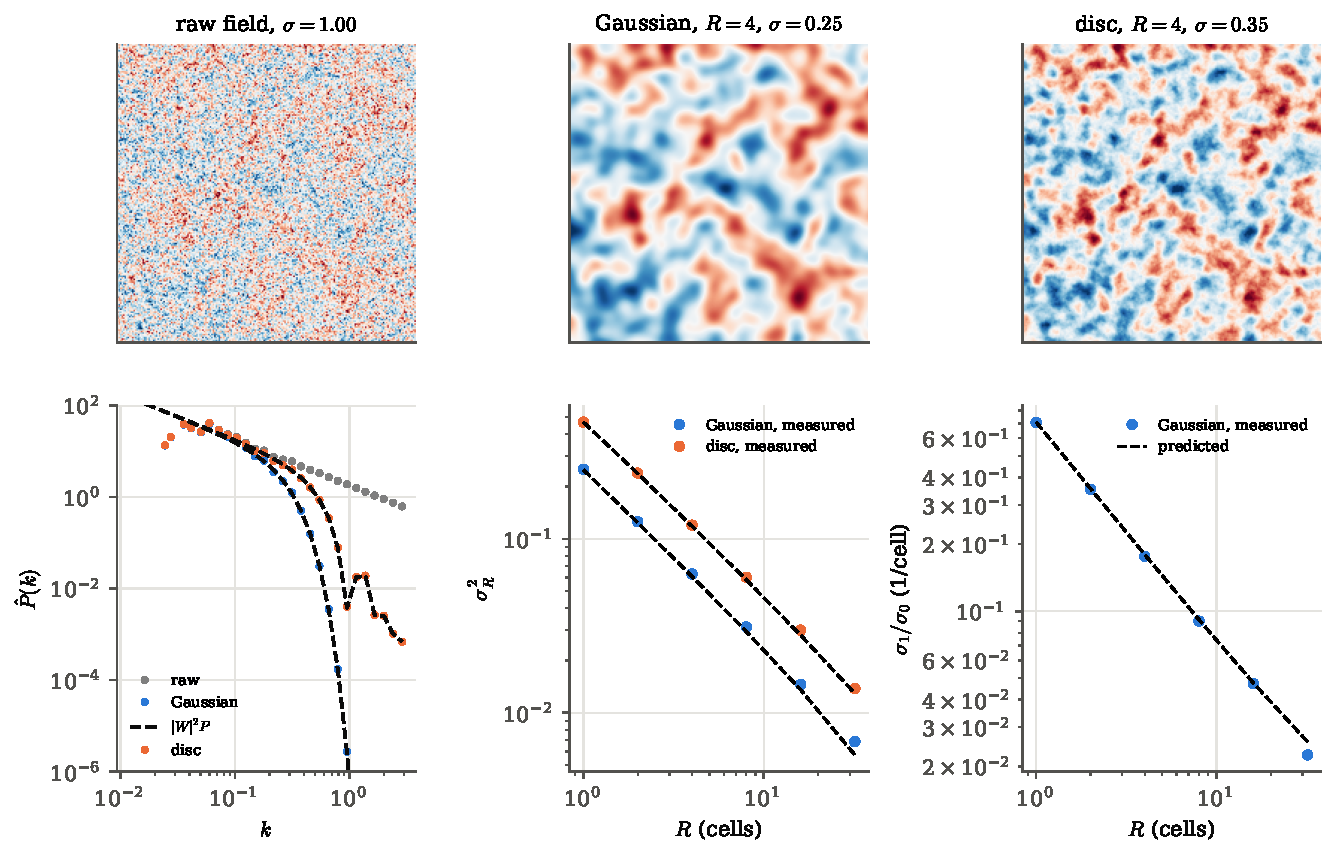
\includegraphics[width=\linewidth]{figures/ch07/smoothing.pdf}
\caption{Smoothing a field with $P\propto k^{-1}$. Top: a corner of the raw map,
and the same map smoothed with a Gaussian and with a disc of radius $4$ cells,
each shown in units of its own standard deviation. Bottom left: the smoothed
spectra follow $|W|^2P$. Bottom middle: $\sigma_R^2$ falls as $1/R$ for both
windows. Bottom right: the ratio $\sigma_1/\sigma_0$, the inverse feature spacing,
falls as $1/(\sqrt2R)$.}
\label{7a:fig:smoothing}
\end{figure}

\subsection{What a beam does to the acoustic peaks}
\label{7a:sec:beam-peaks}

The temperature spectrum of the microwave sky (\cref{ch:T1}) has a flat plateau at the largest
angles and then a train of acoustic peaks, the first at $\ell\approx\SevABmPkA$, the next at
$\SevABmPkB$, $\SevABmPkC$, $\SevABmPkD$, $\SevABmPkE$ and $\SevABmPkF$ in the fiducial model. Here
$\ell$ is the multipole, the sphere's version of a wavenumber: a pattern of multipole $\ell$ has an
angular wavelength of about $2\pi/\ell$ radians, so $\ell=200$ means spots about a degree across.
Its power is $\Cell$, plotted as $D_\ell=\ell(\ell+1)\Cell/2\pi$ (\cref{ch:T1}). Every satellite that
mapped this sky saw it through a beam, and the beams differed by a factor of eighty: about $7^\circ$
for COBE, between $0.9^\circ$ and $0.2^\circ$ for the channels of WMAP, and about $5'$ for the best
Planck channels. \emph{The question.} Which of the peaks can an experiment with a given beam see?

\paragraph{The beam window.}
On a patch of sky small enough to be flat, $\ell$ is the length of a two-dimensional wave vector,
and $\Cell$ plays the role of $P(k)$. A Gaussian beam is the Gaussian window
\eqref{7a:eq:wgauss} with $R=\sigma_b={\rm FWHM}/\sqrt{8\ln2}$, measured in radians. So each
multipole of the sky is multiplied by $B_\ell=e^{-\ell^2\sigma_b^2/2}$, and, since smoothing
multiplies the power by $|W|^2$ (\cref{7a:sec:convolution}), the observed spectrum is
$B_\ell^2\Cell$. On the full sphere the exact form replaces $\ell^2$ by $\ell(\ell+1)$,
$B_\ell^2=e^{-\ell(\ell+1)\sigma_b^2}$, which \cref{ch:08} derives from the Legendre expansion of
the beam.

\emph{Where does the beam cut?} It leaves the large scales alone and removes power above some
multipole. A natural marker is the multipole where it has removed half the power:
\begin{align}
  e^{-\ell(\ell+1)\sigma_b^2}=\tfrac12
  \;&\eqby{1}\;\ell(\ell+1)\,\sigma_b^2=\ln2
  \;\;\relby{2}{\Longrightarrow}\;\;\ell_{1/2}\approx\frac{\sqrt{\ln2}}{\sigma_b}
  \nonumber\\
  &\eqby{3}\frac{\sqrt8\,\ln2}{\rm FWHM}\approx\frac{1.96}{{\rm FWHM}\,[{\rm rad}]}
  \eqby{4}\frac{6740}{{\rm FWHM}\,[{\rm arcmin}]} .
  \label{7a:eq:lhalf}
\end{align}
\begin{explain}
  \item Take minus the logarithm of both sides.
  \item For $\ell\gg1$, $\ell(\ell+1)\approx\ell^2$. The exact positive root,
        $\ell=\bigl(-1+\sqrt{1+4\ln2/\sigma_b^2}\bigr)/2$, is smaller by less than $1/2$.
  \item Insert $\sigma_b={\rm FWHM}/\sqrt{8\ln2}$: $\sqrt{\ln2}\cdot\sqrt{8\ln2}=\sqrt8\,\ln2=1.96$.
  \item One arcminute is $2.909\times10^{-4}$\,rad.
\end{explain}
The amplitude $B_\ell$ (rather than the power $B_\ell^2$) falls to one half at $\sqrt2$ times this
multipole, $\sqrt{2\ln2}/\sigma_b$. A beam twice as narrow reaches twice as far in $\ell$. For the
five beams of \cref{7a:fig:beam-peaks}, script \pyname{code/ch07/10_beam_peaks.py} gives:

\begin{center}
\small
\begin{tabular}{@{}lccccc@{}}
\hline
FWHM & $7^\circ$ & $1^\circ$ & $30'$ & $10'$ & $5'$\\
$\sigma_b$ [arcmin] & $\SevABmSigmaCobe$ & $\SevABmSigmaDeg$ & $\SevABmSigmaThirty$ & $\SevABmSigmaTen$ & $\SevABmSigmaFive$\\
$\ell_{1/2}$ & $\SevABmLhalfCobe$ & $\SevABmLhalfDeg$ & $\SevABmLhalfThirty$ & $\SevABmLhalfTen$ & $\SevABmLhalfFive$\\
peaks with $B_\ell^2>1/2$ & $\SevABmNpkCobe$ & $\SevABmNpkDeg$ & $\SevABmNpkThirty$ & $\SevABmNpkTen$ & $\SevABmNpkFive$\\
deconvolved noise $=$ sky at $\ell$ & $\SevABmLeqCobe$ & $\SevABmLeqDeg$ & $\SevABmLeqThirty$ & $\SevABmLeqTen$ & $\SevABmLeqFive$\\
\hline
\end{tabular}
\end{center}
The exact roots and the approximation \eqref{7a:eq:lhalf} agree to one unit in every case
($\SevABmLhalfApproxFive$ against $\SevABmLhalfFive$ for the $5'$ beam). The left panel of
\cref{7a:fig:beam-peaks} shows the beamed spectra $D_\ell B_\ell^2$. The suppression is exponential
in $\ell^2$, so a beam always takes the highest peaks first: the $10'$ beam keeps the first peak at
$\SevABmBlTenOne\%$ of its power and the fifth at only $\SevABmBlTenFive\%$.

\paragraph{Undoing the beam, and its price.}
The beam is known, so it can be divided out: $\widehat C_\ell/B_\ell^2$ is again an estimate of
the true $\Cell$. The price is noise. The detector noise is added \emph{after} the beam, so dividing
by $B_\ell^2$ also multiplies the noise power by $1/B_\ell^2=e^{\ell(\ell+1)\sigma_b^2}$. White
noise has a flat spectrum, as in the example of smoothing white noise above: pixel noise of
variance $\sigma_n^2$ in cells of solid angle $\Omega$ has $N_\ell=\sigma_n^2\Omega$ for every
$\ell$, and $\sqrt{N_\ell}$ is the map depth, quoted in $\mu$K\,arcmin. So the deconvolved spectrum
is $\Cell+N_\ell/B_\ell^2$ on average, and the second term climbs like $e^{\ell^2\sigma_b^2}$. The right
panel of \cref{7a:fig:beam-peaks} shows it for the same depth, $\SevABmPkDepth\,\mu$K\,arcmin, in
every case: each curve follows the sky until the noise wall rises through it, at the multipole in
the last row of the table. Beyond that point no amount of deconvolution recovers the peaks;
\cref{ch:08} turns this into an error bar.

\paragraph{What each experiment could see.}
A $7^\circ$ beam, COBE's, keeps half the power only up to $\ell\approx\SevABmLhalfCobe$. That is
the Sachs--Wolfe plateau, the flat part of $D_\ell$ at $\ell\lesssim20$ that carries the amplitude
and the tilt of the primordial fluctuations, and nothing of the peaks: at the first peak, $\ell=\SevABmPkA$, the beam leaves
$B_\ell^2=e^{-\ell(\ell+1)\sigma_b^2}\approx10^{-\SevABmCobeExp}$ of the power. WMAP's sharpest
channel had a beam of about $13'$, so $\ell_{1/2}\approx\SevABmLhalfWmap$: the first peak keeps
$\SevABmWmapOne\%$ of its power, the second $\SevABmWmapTwo\%$ and the third only
$\SevABmWmapThree\%$. With its noise wall between those of the $10'$ and $30'$ columns, such a
beam measures the first two peaks well and the third at the edge of its reach. A $5'$
beam, Planck's, keeps half the power up to $\ell\approx\SevABmLhalfFive$, so the first four peaks
pass almost untouched, and the deconvolved noise of a $\SevABmPkDepth\,\mu$K\,arcmin map overtakes
the sky only at $\ell\approx\SevABmLeqFive$: all six peaks of the figure, and the start of the
damping tail beyond them, are within reach. The beam width and the reach in multipoles are two
ways of stating one number: $\ell_{1/2}\approx6740/{\rm FWHM}[']$.

\begin{figure}[htbp]
\centering
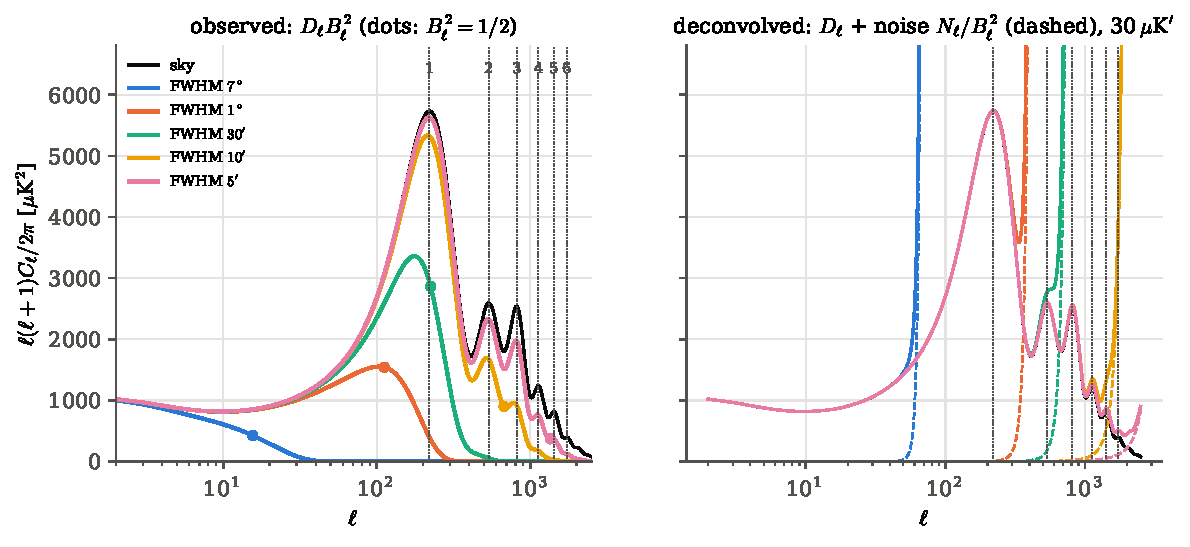
\includegraphics[width=\linewidth]{figures/ch07/beam_peaks.pdf}
\caption{What a beam does to the acoustic peaks. Left: the fiducial spectrum $D_\ell$ (black) seen
through Gaussian beams from $7^\circ$ to $5'$; the dotted lines mark the six peaks and each dot the
multipole $\ell_{1/2}$ where the beam has removed half the power. The higher peaks go first. Right:
the beam divided back out, for white noise of the same depth in every case. The sky is recovered
(solid curves lie on the black one) until the deconvolved noise $N_\ell/B_\ell^2$ (dashed) rises
through it like a wall.}
\label{7a:fig:beam-peaks}
\end{figure}

Smoothing is the first example of an observational effect acting on a summary:
the instrument applies a known linear operation to the field, and the power
spectrum changes in a known way. \Cref{ch:08} adds two effects that are harder
to undo: noise, which adds power, and the mask, which couples modes.
\section{What the power spectrum throws away}
\label{7a:sec:phases}

Imagine a universe in which a first-order phase transition left behind thin
shells, the walls of expanding bubbles, scattered at random. Its density map is a
field of rings. Now take that map, Fourier transform it, keep the amplitude
$|\delta_{\bm k}|$ of every mode exactly, replace every phase by a random number,
and transform back. The result has precisely the same power spectrum as the
rings, mode by mode, and it looks like nothing but Gaussian noise
(\cref{7a:fig:phases-maps}, panels a and b). Any analysis that measures only
$P(k)$ would declare the two universes identical. The physics that made the rings
is invisible to it.

The reason is in the definition of the estimator. Write each mode in polar form,
$\delta_{\bm k}=|\delta_{\bm k}|e^{i\varphi_{\bm k}}$, with amplitude
$|\delta_{\bm k}|$ and phase $\varphi_{\bm k}$. The estimator $\hat P(k)$ of
\eqref{7a:eq:phat} uses $|\delta_{\bm k}|^2$ and nothing else, so it is unchanged
by any change of phases $\varphi_{\bm k}\to\varphi_{\bm k}+\alpha_{\bm k}$ with
$\alpha_{-\bm k}=-\alpha_{\bm k}$ (the restriction keeps the reality condition
\eqref{7a:eq:reality}, so the map stays real). Half of the numbers that describe
the map, one phase per independent mode, are discarded.

\paragraph{The question.} When is discarding the phases harmless, and what do the
phases carry when it is not?

\paragraph{For a Gaussian field the phases are pure noise.}
In \cref{7a:sec:grf-fourier} we found that a homogeneous Gaussian field has
independent, uniformly distributed phases, independent also of the amplitudes.
There is nothing to learn from a uniform random number that the theory already
told us was uniform. This is the Fourier-space form of the result of
\cref{7a:sec:grf}: for a Gaussian field the power spectrum is the whole story.

\paragraph{For a non-Gaussian field the phases carry the shapes.}
In a non-Gaussian field the phases of different modes are \emph{correlated}. A
thin ring is a sum of many plane waves whose crests line up along the ring. That
alignment, a relation between the phases of different $\bm k$, is what makes a
sharp, connected structure instead of a random interference pattern. The same
holds for filaments, walls, clumps and the step-like edges of cosmic strings.

\paragraph{Why random phases look Gaussian.}
Randomising the phases makes almost any field look Gaussian. Each pixel of the
randomised map is a sum over many modes,
$\delta(\bm x)=\frac1V\sum_{\bm k}|\delta_{\bm k}|\cos(\bm k\cdot\bm x+\varphi_{\bm k})$
(pairing $\pm\bm k$), and the phases are now independent random numbers. By the
central limit theorem (\cref{ch:02}) a sum of many independent terms is close to
Gaussian, whatever the amplitudes. So, as long as the power is spread over many
modes, phase randomisation gives an almost Gaussian field with the same power
spectrum.

\paragraph{Seeing it.}
The script \pyname{code/ch07/09_phases.py} builds a map of $\SevANRings$ thin rings
of random radii on a $256\times256$ periodic grid, standardised to zero mean and unit
variance, and its phase-randomised twin. The phases are taken from the FFT of
fresh white noise, which has the Hermitian symmetry built in, so the twin is real
automatically:

\pyfile[firstline=154,lastline=165,firstnumber=154]{code/ch07/lib_fields.py}{Phase
randomisation: keep $|\delta_{\bm k}|$, draw new phases}

Lines 160--161 transform the map and a white-noise map of the same size. Line 162
reduces the white-noise modes to unit complex numbers, whose phases are uniform
(\cref{7a:sec:grf-fourier}) and already satisfy $u_{-\bm k}=u_{\bm k}^*$. Line 163
attaches them to the old amplitudes, line 164 keeps the $\bm k=0$ mode (the mean),
and line 165 transforms back.

The two maps have the same $\hat P(k)$ to $\SevAPkMaxDiff$, rounding error
(\cref{7a:fig:phases-stats}, left). Everything else differs.
\emph{The one-point distribution.} For the rings it is strongly skewed, with
skewness $\SevASkewRings$: most pixels sit on the flat background just below the
mean, and a few on the bright rings. The twin has skewness $\SevASkewShuf$ and a
Gaussian histogram, as the central-limit argument says.
\emph{The excursion sets} differ most of all. Count the connected regions where
the field exceeds $\nu$ standard deviations (\pyname{scipy.ndimage.label} labels
the connected clusters of pixels). At $\nu=1$ the rings give $\SevACompRingsOne$
regions, chains of overlapping rings; their Gaussian twin gives
$\SevACompShufOne$ small blobs. The ring curve has a sharp spike near
$\nu\approx1.6$, the crest height of a single ring. The grid samples each crest
at slightly different heights. So a threshold just below the crest height chops
every ring into many short arcs, while a threshold just above it leaves only the
places where rings overlap.

\begin{figure}[htbp]
\centering
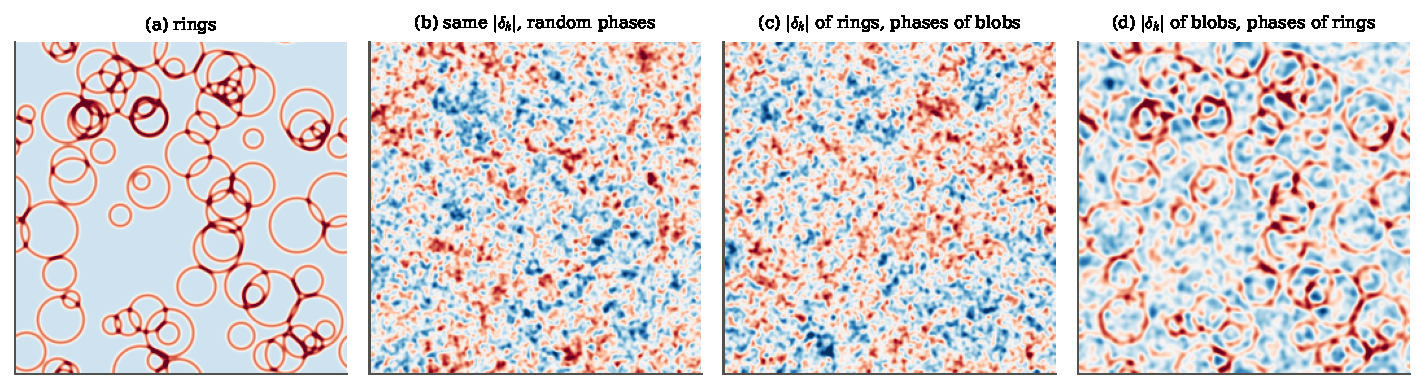
\includegraphics[width=\linewidth]{figures/ch07/phases_flat_maps.pdf}
\caption{Amplitudes and phases. (a) A field of thin rings. (b) The same Fourier
amplitudes with random phases: the same power spectrum, and the rings are gone.
(c) The amplitudes of the rings with the phases of a Gaussian blob field: the
phases are random, and so is the picture. (d) The amplitudes of the blob field with
the phases of the rings: the rings come back. Where structures are, and what shape
they have, is written in the phases.}
\label{7a:fig:phases-maps}
\end{figure}

\begin{figure}[htbp]
\centering
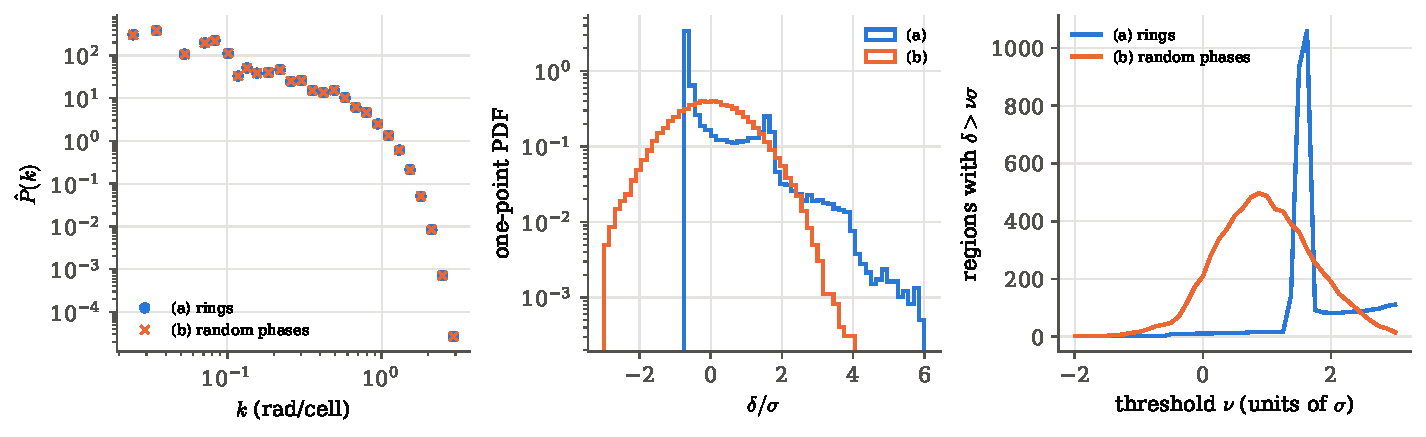
\includegraphics[width=\linewidth]{figures/ch07/phases_flat_stats.pdf}
\caption{Three summaries of the ring map (a) and its phase-randomised twin (b).
Left: identical power spectra. Middle: very different one-point distributions,
skewed for the rings, Gaussian for the twin. Right: the number of connected
regions above a threshold $\nu$, which tells the two apart at all but the lowest and highest thresholds.}
\label{7a:fig:phases-stats}
\end{figure}

The amplitudes say how much of each scale is present; the phases say where it is
and how it is arranged. The phase swap in \cref{7a:fig:phases-maps}(c, d) shows
this directly. Give the ring map's amplitudes the phases of a Gaussian blob field,
and the result is another random-looking Gaussian pattern: the phases of a
Gaussian field are random, and they decide what the picture looks like. Give the
blob amplitudes the ring phases, and the rings reappear, blurred because the blob
amplitudes are weak at high $k$.

\subsection{A taxonomy of summaries}
\label{7a:sec:taxonomy}

The power spectrum is one choice of what to measure. Given a field
$\phi:\mathcal M\to\R$ on a domain $\mathcal M$, the summaries used in physics fall
into a few families, each answering a different question about the same data:
\begin{equation}
  \phi
  \longrightarrow
  \left\{
  \begin{array}{ll}
    \text{amplitude} & \langle\phi\rangle,\ \Var(\phi),\ P(\phi),\\
    \text{correlation} & \xi(r),\ P(k),\ \Cell,\\
    \text{higher-order structure} & B,\ T,\ldots,\\
    \text{geometry/morphology} & \text{sizes, shapes, curvature, excursion geometry},\\
    \text{topology} & \beta_i,\ \chi,\ \text{persistence}.
  \end{array}\right.
  \label{7a:eq:taxonomy}
\end{equation}
Each row answers its own question.
\emph{Amplitude:} how large is the field typically? It is read from the one-point
distribution $P(\phi)$; the skewness above is an amplitude statistic.
\emph{Correlation:} how are values at different places related? This is
everything for a Gaussian field, and blind to phases.
\emph{Higher-order structure:} the three- and four-point functions and their
Fourier transforms, the bispectrum $B$ and trispectrum $T$. The failed Wick test
of the lognormal field in \cref{7a:fig:gaussian-checks} was a four-point
statistic.
\emph{Geometry and topology:} what shapes does the field make in real space? An
example is the excursion set $\{\bm x:\phi(\bm x)>\nu\}$, whose connected pieces
we just counted. In topology $\beta_0$ counts connected components, $\beta_1$
counts holes, and $\chi$, the Euler characteristic, combines them
(\cref{ch:12}).

Each of these summaries $S$, once chosen, is an ordinary random variable.
Repeated universes give it a sampling distribution $P(S\given\theta)$, with
$\theta$ the parameters of the theory, and the machinery of the rest of the book
applies to it unchanged.

The ring example raises the question behind the last row. Is there physical
information in the way the regions of a field are connected that the statistic
we are already using, here the power spectrum, does not expose? For the rings the
answer is plainly yes, and the region count of \cref{7a:fig:phases-stats}
already sees it. \Cref{ch:12} builds that observation into a method: excursion sets at every threshold, their Betti numbers and Euler
characteristic, and persistence, the record of how long each structure survives as
the threshold moves. It also turns them into statistics with sampling
distributions computed from exactly the Gaussian simulations of
\cref{7a:sec:simulate}, because a Gaussian field with the measured $P(k)$ is the
natural null hypothesis: it is the field that contains the two-point information
and nothing else.

\begin{inpractice}[Simulated Gaussian fields: verification and research]
Every simulation of a flat Gaussian field above has been a \emph{verification}: we knew the answer
analytically (the Wiener--Khinchin theorem, the recipe's normalisation, the
exponential distribution of a mode, $\sqrt{2/N_{\rm modes}}$, $|W|^2P$) and the
simulation confirmed it, which is how one tests both the code and one's
understanding. In research the same machinery is the instrument itself, used where
no formula exists. Survey analyses estimate the covariance of $\hat P(k)$ or
$\hat\xi(r)$ including the survey window, non-linear evolution and galaxy bias from
hundreds to thousands of mock catalogues, typically generated from Gaussian or
lognormal fields made exactly as in \cref{7a:sec:simulate} or from $N$-body runs; the
finite number of mocks itself biases the inverse covariance, and corrections for
it are standard \cite{Hartlap2007,Taylor2013}. Searches for non-Gaussianity in the
CMB compare the data with large sets of Gaussian simulations that share the
measured power spectrum \cite{Planck2018IX}; phase-randomised ``surrogate'' maps
play the same role for any field. On the sphere, the transfer of power by the
mask and beam is calibrated on simulated skies (\cref{ch:08}).
\end{inpractice}

The two-point summaries are where the analysis of a field starts and, for a
Gaussian field, where it ends. On the sky the plane waves become spherical
harmonics, the power spectrum becomes $\Cell$, and the mode counting of
\cref{7a:sec:sample-var} becomes cosmic variance; that is the CMB's version of
the same story.

\begin{recap}
\begin{itemize}
  \item A theory predicts the statistics of a field, not the field. A random field is a
        random variable at every point, specified by its $n$-point distributions; the
        ensemble is the stack of possible universes.
  \item Homogeneity and isotropy make the covariance a function of distance only,
        $\xi(r)=\langle\delta(\bm x)\delta(\bm x+\bm r)\rangle$, with $\xi(0)=\sigma^2$,
        $|\xi|\le\xi(0)$, and positive definiteness.
  \item A Gaussian field is fixed by $\xi$: the joint law of any set of points is
        $\Normal(\bm0,\Cmat)$ with $\Cmat_{ij}=\xi(r_{ij})$; the mean field around a
        hot spot is $\nu\xi(r)/\sigma$; four-point moments are sums over pairings (Wick).
  \item Fourier modes of a homogeneous field are uncorrelated,
        $\langle\delta_{\bm k}\delta_{\bm k'}^*\rangle=(2\pi)^d\delta_D(\bm k-\bm k')P(k)$,
        with $P$ the Fourier transform of $\xi$ (Wiener--Khinchin) and $P\ge0$. For a
        Gaussian field each mode has an exponential power and a uniform phase.
  \item Simulation: FFT white noise, multiply by $\sqrt{P(k)/\Delta^d}$, inverse FFT;
        a box holds only $k_f\le k\le k_{\rm Ny}$ and has zero mean.
  \item One universe: spatial averages replace ensemble averages only for ergodic
        fields; the mean over a volume has variance $P(0)/V$; a shell-averaged
        power spectrum has $\Delta\hat P/P=\sqrt{2/N_{\rm modes}}$, even without noise.
  \item Smoothing by a window multiplies the spectrum by $|W(k)|^2$; the spectral
        moments $\sigma_j$ set the variance, the gradients and the feature spacing.
  \item $P(k)$ discards the phases. For a Gaussian field they are noise; for any other
        field they hold the shapes, which morphology and topology (\cref{ch:12}) measure.
\end{itemize}
\end{recap}
\providecommand{\SBdipA}{}\renewcommand{\SBdipA}{3}
\providecommand{\SBdipTh}{}\renewcommand{\SBdipTh}{6.139960}
\providecommand{\SBdipNum}{}\renewcommand{\SBdipNum}{6.139960}
\providecommand{\SBdipOther}{}\renewcommand{\SBdipOther}{1.009\times10^{-15}}
\providecommand{\SBnRealSix}{}\renewcommand{\SBnRealSix}{361197}
\providecommand{\SBnStoredSix}{}\renewcommand{\SBnStoredSix}{180901}
\providecommand{\SBvarZero}{}\renewcommand{\SBvarZero}{12635}
\providecommand{\SBrmsZero}{}\renewcommand{\SBrmsZero}{112.4}
\providecommand{\SBfracLowL}{}\renewcommand{\SBfracLowL}{19.9}
\providecommand{\SBisoNsim}{}\renewcommand{\SBisoNsim}{6000}
\providecommand{\SBisoAmp}{}\renewcommand{\SBisoAmp}{0.5}
\providecommand{\SBisoPowDevMax}{}\renewcommand{\SBisoPowDevMax}{0.02503}
\providecommand{\SBisoErr}{}\renewcommand{\SBisoErr}{0.01291}
\providecommand{\SBisoXmax}{}\renewcommand{\SBisoXmax}{0.01502}
\providecommand{\SBmodPowZero}{}\renewcommand{\SBmodPowZero}{1.126}
\providecommand{\SBmodXzero}{}\renewcommand{\SBmodXzero}{0.5005}
\providecommand{\SBpBelowMean}{}\renewcommand{\SBpBelowMean}{0.5841}
\providecommand{\SBpFifth}{}\renewcommand{\SBpFifth}{0.03743}
\providecommand{\SBpThirty}{}\renewcommand{\SBpThirty}{0.1299}
\providecommand{\SBfracTwo}{}\renewcommand{\SBfracTwo}{0.6325}
\providecommand{\SBfracThirty}{}\renewcommand{\SBfracThirty}{0.1811}
\providecommand{\SBfracThousand}{}\renewcommand{\SBfracThousand}{0.03161}
\providecommand{\SBfracBinned}{}\renewcommand{\SBfracBinned}{0.4471}
\providecommand{\SBskewTwo}{}\renewcommand{\SBskewTwo}{1.265}
\providecommand{\SBloTwo}{}\renewcommand{\SBloTwo}{0.56}
\providecommand{\SBhiTwo}{}\renewcommand{\SBhiTwo}{2.03}
\providecommand{\SBloHund}{}\renewcommand{\SBloHund}{0.91}
\providecommand{\SBhiHund}{}\renewcommand{\SBhiHund}{1.11}
\providecommand{\SBpeakEll}{}\renewcommand{\SBpeakEll}{220}
\providecommand{\SBpeakD}{}\renewcommand{\SBpeakD}{5732}
\providecommand{\SBlmaxBand}{}\renewcommand{\SBlmaxBand}{2500}
\providecommand{\SBnpixTwoFiveSix}{}\renewcommand{\SBnpixTwoFiveSix}{786432}
\providecommand{\SBnpixFiveTwelve}{}\renewcommand{\SBnpixFiveTwelve}{3145728}
\providecommand{\SBnpixTwoK}{}\renewcommand{\SBnpixTwoK}{50{,}331{,}648}
\providecommand{\SBpixTwoFiveSix}{}\renewcommand{\SBpixTwoFiveSix}{13.74}
\providecommand{\SBpixFiveTwelve}{}\renewcommand{\SBpixFiveTwelve}{6.871}
\providecommand{\SBpixTwoK}{}\renewcommand{\SBpixTwoK}{1.718}
\providecommand{\SBourVsHp}{}\renewcommand{\SBourVsHp}{6.474\times10^{-16}}
\providecommand{\SBrtZero}{}\renewcommand{\SBrtZero}{2.272\times10^{-5}}
\providecommand{\SBrtThree}{}\renewcommand{\SBrtThree}{1.116\times10^{-8}}
\providecommand{\SBrtThreeMax}{}\renewcommand{\SBrtThreeMax}{3.973\times10^{-7}}
\providecommand{\SBrtAlias}{}\renewcommand{\SBrtAlias}{2.213\times10^{-6}}
\providecommand{\SBNsim}{}\renewcommand{\SBNsim}{20{,}000}
\providecommand{\SBNbig}{}\renewcommand{\SBNbig}{10^6}
\providecommand{\SBksTwo}{}\renewcommand{\SBksTwo}{0.2452}
\providecommand{\SBksTen}{}\renewcommand{\SBksTen}{0.8436}
\providecommand{\SBksFifty}{}\renewcommand{\SBksFifty}{0.3608}
\providecommand{\SBksThree}{}\renewcommand{\SBksThree}{0.6115}
\providecommand{\SBvrTwo}{}\renewcommand{\SBvrTwo}{1.021}
\providecommand{\SBvrTen}{}\renewcommand{\SBvrTen}{1.000}
\providecommand{\SBvrFifty}{}\renewcommand{\SBvrFifty}{1.015}
\providecommand{\SBvrThree}{}\renewcommand{\SBvrThree}{0.998}
\providecommand{\SBerrTwo}{}\renewcommand{\SBerrTwo}{0.01483}
\providecommand{\SBerrThree}{}\renewcommand{\SBerrThree}{0.01005}
\providecommand{\SBmeanDevMax}{}\renewcommand{\SBmeanDevMax}{3.081}
\providecommand{\SBslopeHi}{}\renewcommand{\SBslopeHi}{-0.5133}
\providecommand{\SBslopeTwo}{}\renewcommand{\SBslopeTwo}{-0.5011}
\providecommand{\SBcoefTwo}{}\renewcommand{\SBcoefTwo}{2.098}
\providecommand{\SBoffSdFiveH}{}\renewcommand{\SBoffSdFiveH}{0.04741}
\providecommand{\SBoffInvFiveH}{}\renewcommand{\SBoffInvFiveH}{0.04472}
\providecommand{\SBoffSdAll}{}\renewcommand{\SBoffSdAll}{0.007064}
\providecommand{\SBoffInvAll}{}\renewcommand{\SBoffInvAll}{0.007071}
\providecommand{\SBoffMaxBig}{}\renewcommand{\SBoffMaxBig}{0.02929}
\providecommand{\SBnOffBig}{}\renewcommand{\SBnOffBig}{44551}
\providecommand{\SBknoxErr}{}\renewcommand{\SBknoxErr}{7.1}
\providecommand{\SBhpN}{}\renewcommand{\SBhpN}{3000}
\providecommand{\SBhpKsTwo}{}\renewcommand{\SBhpKsTwo}{0.5166}
\providecommand{\SBhpKsTen}{}\renewcommand{\SBhpKsTen}{0.998}
\providecommand{\SBhpKsFifty}{}\renewcommand{\SBhpKsFifty}{0.9504}
\providecommand{\SBhpVrTwo}{}\renewcommand{\SBhpVrTwo}{0.973}
\providecommand{\SBhpVrFifty}{}\renewcommand{\SBhpVrFifty}{0.996}
\providecommand{\SBphNspot}{}\renewcommand{\SBphNspot}{40}
\providecommand{\SBphMaxDiff}{}\renewcommand{\SBphMaxDiff}{5.322\times10^{-16}}
\providecommand{\SBphSkewA}{}\renewcommand{\SBphSkewA}{2.903}
\providecommand{\SBphSkewB}{}\renewcommand{\SBphSkewB}{0.01184}
\section{The Fourier modes of the sphere}
\label{7b:sec:harmonics}

Point a radio telescope tuned to millimetre wavelengths at any direction on the sky and it
records a temperature of about $2.7255$\,K. Subtract that average and what remains is a pattern
of hot and cold patches, typically about a hundred microkelvin above or below the average (that
is the rms). This pattern is the cosmic microwave background (CMB) anisotropy. It is a random
field on the sky: one real number $\Theta(\bm e)$ for every direction $\bm e$. The number is the
temperature contrast $\delta T/T$. We always quote it multiplied by
$T_0=2.7255\times10^6\,\mu$K, so that $\Theta$ and everything built from it are in microkelvin,
the units CAMB uses (\cref{ch:T1}).

For fields in flat space (\cref{7a:sec:fourier,7a:sec:wk}) the key step was to expand the
field in plane waves $e^{i\bm k\cdot\bm x}$. Each plane wave is a pattern of one definite
wavelength. Homogeneity made the amplitudes of different plane waves uncorrelated, and the
variance of each amplitude was the power spectrum $P(k)$. The sky, however, is a sphere, and a
sphere has no plane waves: $e^{i\bm k\cdot\bm x}$ has no meaning on a curved, closed surface. So
before any statistics we need a piece of geometry.

\paragraph{The question.} Which patterns on the sphere play the role that plane waves play in
flat space: patterns of a definite angular size, from which any sky can be built, and which a
rotation of the sky only shuffles among themselves?

\subsection{Spherical harmonics: what they are and why they are the right modes}
\label{7b:sec:ylm}

The answer is the spherical harmonics. To see why, ask first what makes a plane wave special.
It is an eigenfunction of the Laplacian:
$\nabla^2e^{i\bm k\cdot\bm x}=-k^2e^{i\bm k\cdot\bm x}$. The eigenvalue $-k^2$ measures how
rapidly the pattern wiggles, and $2\pi/k$ is its wavelength. The Laplacian also makes sense on
the unit sphere, so the natural replacement for plane waves is the eigenfunctions of the
Laplacian on the sphere,
\begin{equation}
  \nabla^2_{S^2}\,Y = \frac{1}{\sin\theta}\frac{\partial}{\partial\theta}
  \Bigl(\sin\theta\,\frac{\partial Y}{\partial\theta}\Bigr)
  +\frac{1}{\sin^2\theta}\frac{\partial^2Y}{\partial\phi^2}
  = -\ell(\ell+1)\,Y ,
  \label{7b:eq:laplace-sphere}
\end{equation}
where $\theta\in[0,\pi]$ is the colatitude (angle from the north pole) and $\phi\in[0,2\pi)$ the
longitude of the direction $\bm e$. We have met these functions before: they are the
angular parts of the hydrogen wavefunctions. In quantum mechanics (with $\hbar=1$) the orbital
angular momentum $\bm L=-i\,\bm r\times\bm\nabla$ satisfies $\bm L^2=-\nabla^2_{S^2}$, and the
\newterm{spherical harmonics} $Y_{\ell m}(\theta,\phi)$ are the simultaneous eigenfunctions
\begin{equation}
  \bm L^2\,Y_{\ell m}=\ell(\ell+1)\,Y_{\ell m},\qquad
  L_z\,Y_{\ell m}=m\,Y_{\ell m},\qquad
  \ell=0,1,2,\dots,\quad m=-\ell,\dots,\ell ,
  \label{7b:eq:ylm-eigen}
\end{equation}
with $L_z=-i\,\partial/\partial\phi$. So $Y_{\ell m}\propto e^{im\phi}$, and in general
$Y_{\ell m}(\theta,\phi)=N_{\ell m}P_\ell^m(\cos\theta)\,e^{im\phi}$, with $P_\ell^m$ an
associated Legendre function and $N_{\ell m}$ a normalisation constant. We use the standard
(Condon--Shortley) phase convention of quantum mechanics, the one healpy and CAMB also use. The
first few, written out so that we can compute with them, are
\begin{equation}
\begin{aligned}
  Y_{00}&=\frac{1}{\sqrt{4\pi}}, &
  Y_{10}&=\sqrt{\frac{3}{4\pi}}\cos\theta, &
  Y_{1,\pm1}&=\mp\sqrt{\frac{3}{8\pi}}\sin\theta\,e^{\pm i\phi},\\
  Y_{20}&=\sqrt{\frac{5}{16\pi}}\,(3\cos^2\theta-1), &
  Y_{2,\pm1}&=\mp\sqrt{\frac{15}{8\pi}}\sin\theta\cos\theta\,e^{\pm i\phi}, &
  Y_{2,\pm2}&=\sqrt{\frac{15}{32\pi}}\sin^2\theta\,e^{\pm 2i\phi}.
\end{aligned}
\label{7b:eq:ylm-explicit}
\end{equation}

Three properties of the $Y_{\ell m}$ are all we will use.
\begin{enumerate}[itemsep=2pt]
\item \textbf{Orthonormality.} With $\dd\Omega=\sin\theta\,\dd\theta\,\dd\phi$ the solid-angle
  element,
  \begin{equation}
    \int\dd\Omega\;Y_{\ell m}(\bm e)\,Y^*_{\ell'm'}(\bm e)=\delta_{\ell\ell'}\delta_{mm'} .
    \label{7b:eq:orthonormal}
  \end{equation}
  In quantum mechanics this is $\braket{\ell m}{\ell'm'}=\delta_{\ell\ell'}\delta_{mm'}$:
  eigenfunctions of a Hermitian operator with different eigenvalues are orthogonal.
\item \textbf{Completeness.} Any square-integrable function on the sphere is a sum of
  $Y_{\ell m}$'s, just as any periodic function is a Fourier series.
\item \textbf{Complex conjugation flips $m$.} Since $e^{im\phi}$ becomes $e^{-im\phi}$ and the
  Condon--Shortley phase carries a sign $(-1)^m$,
  \begin{equation}
    Y^*_{\ell m}=(-1)^m\,Y_{\ell,-m} .
    \label{7b:eq:ylm-conj}
  \end{equation}
  Check it on \eqref{7b:eq:ylm-explicit}: $Y_{11}^*=-\sqrt{3/8\pi}\sin\theta\,e^{-i\phi}=-Y_{1,-1}$,
  which is $(-1)^1Y_{1,-1}$.
\end{enumerate}

What do $\ell$ and $m$ mean on the sky? In short, $\ell$ sets the angular size of the pattern
and $m$ sets how its zero lines are oriented. \Cref{7b:fig:ylm-gallery} shows the real parts of
six harmonics in the Mollweide projection, the equal-area map of the whole sky in which the
equator is the horizontal midline and the poles are the top and bottom points. The real part of
$Y_{\ell m}$ has $\ell$ nodal lines (lines where it is zero) in total: $m$ of them are great circles through the poles
(the factor $\cos m\phi$ vanishes on $2m$ half-meridians) and $\ell-|m|$ are circles of
constant latitude (the zeros of $P_\ell^m$). The $m=0$ harmonics depend on latitude only
(``zonal''), the $|m|=\ell$ ones on longitude only (``sectoral''), and the rest form a
chessboard (``tesseral''). In every case the distance between neighbouring nodal lines is about
$\pi/\ell$ radians, so
\begin{equation}
  \text{multipole }\ell\ \longleftrightarrow\ \text{angular scale }\vartheta\approx\frac{\pi}{\ell}
  =\frac{180^\circ}{\ell}.
  \label{7b:eq:ell-angle}
\end{equation}
This is the sphere's version of ``wavenumber $k$ $\leftrightarrow$ half-wavelength $\pi/k$''.

\begin{figure}[htbp]
\centering
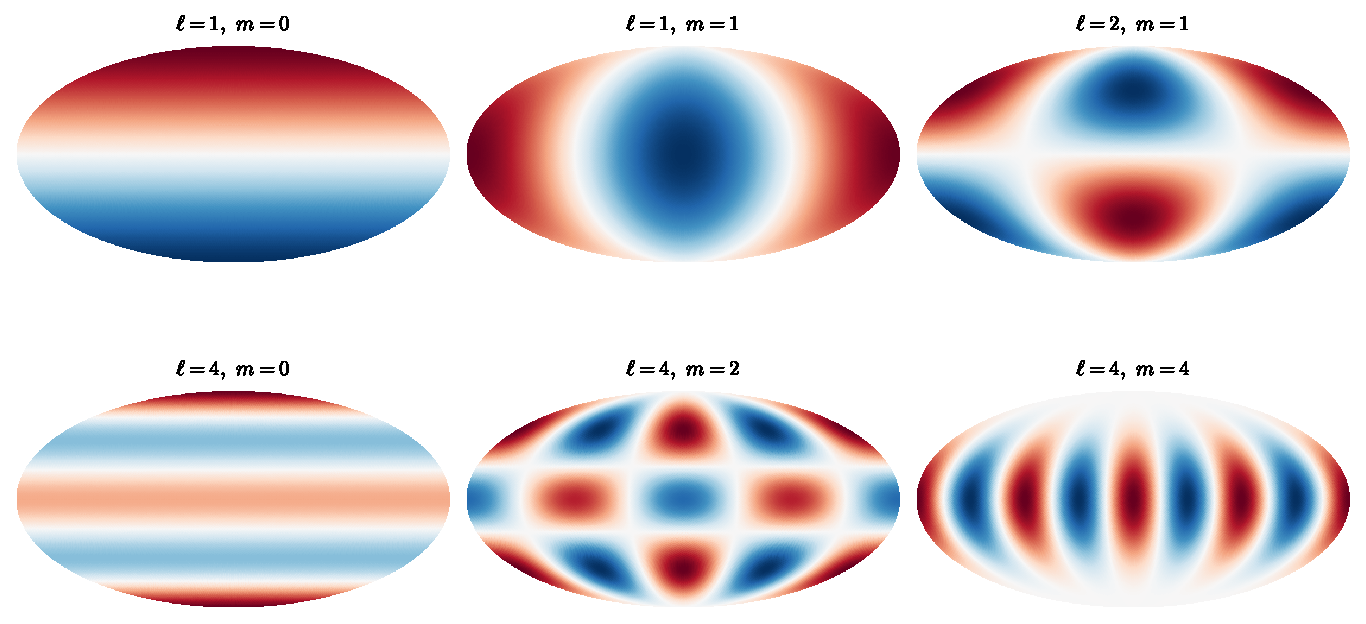
\includegraphics[width=0.95\linewidth]{figures/ch07/ylm_gallery.pdf}
\caption{Real parts of six spherical harmonics on the whole sky (Mollweide projection, north
pole at the top; red positive, blue negative). Top row: the $\ell=1$ dipole along the
pole ($m=0$) and along the equator ($m=1$), and a quadrupole with $m=1$. Bottom row: three
$\ell=4$ harmonics. With $m=0$ the pattern has four latitude rings of zeros; with $m=4$ it has
eight half-meridians of zeros; $m=2$ mixes the two. All three bottom patterns have the same
angular scale, about $180^\circ/4=45^\circ$.}
\label{7b:fig:ylm-gallery}
\end{figure}

\subsection{Expanding a sky: the coefficients $\alm$}
\label{7b:sec:alm}

Completeness (property 2 above) lets us write any sky as a sum of harmonics, and
orthonormality (property 1) tells us how to find the coefficients. Every CMB analysis starts
with this step \srcref{HobsonBMC}{(10.2)}, \srcref{Hivon}{(4)--(5)}.

\begin{workdef}[spherical-harmonic coefficients]
A sky $\Theta(\bm e)$ is expanded as
\begin{equation}
  \Theta(\bm e)=\sum_{\ell=0}^{\infty}\sum_{m=-\ell}^{\ell}\alm\,Y_{\ell m}(\bm e),
  \qquad
  \alm=\int\dd\Omega\;\Theta(\bm e)\,Y^*_{\ell m}(\bm e).
  \label{7b:eq:alm}
\end{equation}
The coefficient $\alm$ \unpack{one complex number per $(\ell,m)$, the overlap of the sky with the
pattern $Y_{\ell m}$} measures how much of the pattern $Y_{\ell m}$ the sky contains.
\emph{Operationally:} multiply the map pixel by pixel by $Y^*_{\ell m}$, multiply by the pixel
area, and add up (\cref{7b:sec:healpix}).
\end{workdef}

Why is the coefficient given by that integral? Because the harmonics are orthonormal, so
projecting the sky onto one harmonic picks out its coefficient and nothing else. In steps:
multiply the expansion by $Y^*_{\ell'm'}(\bm e)$ and integrate over the sky,
\begin{align}
  \int\dd\Omega\;\Theta(\bm e)\,Y^*_{\ell'm'}(\bm e)
  &\eqby{1}\sum_{\ell m}\alm\int\dd\Omega\;Y_{\ell m}(\bm e)\,Y^*_{\ell'm'}(\bm e)
   \eqby{2}\sum_{\ell m}\alm\,\delta_{\ell\ell'}\delta_{mm'}
   \eqby{3}a_{\ell'm'} .
   \label{7b:eq:alm-proof}
\end{align}
\begin{explain}
  \item Insert the expansion and exchange the (convergent) sum with the integral.
  \item Orthonormality \eqref{7b:eq:orthonormal}.
  \item The Kronecker deltas keep only the term $\ell=\ell'$, $m=m'$.
\end{explain}
Cosmological analyses ignore the first two multipoles and start at $\ell=2$
\srcref{HobsonBMC}{p.~230}. The reason is that neither carries the primordial pattern. The
monopole $a_{00}$ is $\sqrt{4\pi}$ times the sky average (because $Y_{00}=1/\sqrt{4\pi}$), and
we subtracted that average. The dipole $\ell=1$ is dominated by our own motion through the CMB,
which Doppler-shifts the temperature by a few millikelvin.

\paragraph{The sky is real, so half of the coefficients are redundant.} The $\alm$ are complex,
but a temperature is a real number, $\Theta^*=\Theta$. What does that imply for the
coefficients? Each negative-$m$ coefficient is fixed by its positive-$m$ partner:
\begin{align}
  a_{\ell,-m}
  &\eqby{1}\int\dd\Omega\;\Theta\,Y^*_{\ell,-m}
   \eqby{2}\int\dd\Omega\;\Theta\,(-1)^mY_{\ell m}
   \eqby{3}(-1)^m\Bigl(\int\dd\Omega\;\Theta\,Y^*_{\ell m}\Bigr)^{\!*}
   \eqby{4}(-1)^m\,\alm^* .
   \label{7b:eq:reality}
\end{align}
\begin{explain}
  \item Definition \eqref{7b:eq:alm} with $m\to-m$.
  \item Conjugate \eqref{7b:eq:ylm-conj}: $Y^*_{\ell,-m}=(-1)^{-m}Y_{\ell m}=(-1)^mY_{\ell m}$.
  \item $\Theta$ is real, so $\Theta Y_{\ell m}=(\Theta Y^*_{\ell m})^*$, and the conjugate can be
        taken outside the integral.
  \item Definition \eqref{7b:eq:alm} again.
\end{explain}
Two consequences follow. For $m=0$, \eqref{7b:eq:reality} reads
$a_{\ell0}=a_{\ell0}^*$, so \emph{$a_{\ell0}$ is real}. For $m\neq0$ the negative-$m$ coefficients
carry no new information, because the positive-$m$ ones fix them. So at each multipole $\ell$
the sky is described by
\begin{equation}
  \underbrace{1}_{a_{\ell0}\ \text{real}}
  +\underbrace{2\ell}_{\mathrm{Re}\,\alm,\ \mathrm{Im}\,\alm,\ m=1,\dots,\ell}
  =2\ell+1\ \text{real numbers}.
  \label{7b:eq:count}
\end{equation}
This count becomes the number of degrees of freedom of the power-spectrum estimator in
\cref{7b:sec:chat}. A second way to reach it: count the independent real patterns at multipole
$\ell$. They are the real and imaginary parts of the $Y_{\ell m}$ with $m\ge0$, which is
$2(\ell+1)$ functions, minus $\mathrm{Im}\,Y_{\ell0}$, which is identically zero. That leaves
$2\ell+1$, the same number. A real sky
band-limited to $\ell\le\ell_{\max}$ is therefore $\sum_{\ell=0}^{\ell_{\max}}(2\ell+1)=(\ell_{\max}+1)^2$ real
numbers. Libraries store only $m\ge0$: $(\ell_{\max}+1)(\ell_{\max}+2)/2$ complex numbers.

\paragraph{The total power of a sky.} How much of a sky's variance sits at each multipole? The
mean square of the sky over the sphere is a sum of $|\alm|^2$. This is the sphere's version of
Parseval's theorem:
\begin{align}
  \frac{1}{4\pi}\int\dd\Omega\;\Theta^2(\bm e)
  &\eqby{1}\frac{1}{4\pi}\sum_{\ell m}\sum_{\ell'm'}\alm\,a^*_{\ell'm'}
     \int\dd\Omega\;Y_{\ell m}Y^*_{\ell'm'}
   \eqby{2}\frac{1}{4\pi}\sum_{\ell}\sum_{m=-\ell}^{\ell}|\alm|^2 .
   \label{7b:eq:parseval}
\end{align}
\begin{explain}
  \item Write $\Theta^2=\Theta\,\Theta^*$ and expand the first factor in $Y_{\ell m}$ and the
        second in $Y^*_{\ell'm'}$ (the conjugate of the expansion, since $\Theta$ is real).
  \item Orthonormality collapses the double sum to $\ell=\ell'$, $m=m'$.
\end{explain}
So $\sum_m|\alm|^2$ (divided by $4\pi$) is the share of the sky's mean square that lives at
angular scale $\pi/\ell$. Divided by the number of terms, $2\ell+1$, it will be our estimator
$\Chat$ of the power spectrum (\cref{7b:sec:chat}).

\paragraph{Example: the dipole along the pole.} Take $\Theta(\bm e)=A\cos\theta$, hot in the
north and cold in the south, with $A$ the temperature at the north pole. The pattern has the
shape of $Y_{10}=\sqrt{3/4\pi}\cos\theta$, so we expect only $a_{10}$ to be nonzero. Its value is
\begin{align}
  a_{10}
  &\eqby{1}\int\dd\Omega\;A\cos\theta\,\sqrt{\frac{3}{4\pi}}\cos\theta
   \eqby{2}A\sqrt{\frac{3}{4\pi}}\;2\pi\int_{-1}^{1}\mu^2\,\dd\mu
   \eqby{3}A\sqrt{\frac{3}{4\pi}}\;\frac{4\pi}{3}
   =A\sqrt{\frac{4\pi}{3}} ,
   \label{7b:eq:dipole}
\end{align}
\begin{explain}
  \item Definition \eqref{7b:eq:alm}; $Y_{10}$ is real.
  \item Substitute $\mu=\cos\theta$, $\dd\Omega=\dd\mu\,\dd\phi$; the $\phi$ integral gives $2\pi$.
  \item $\int_{-1}^1\mu^2\dd\mu=2/3$.
\end{explain}
and every other $\alm$ vanishes, because $\cos\theta$ is proportional to $Y_{10}$ and $Y_{10}$
is orthogonal to all the other $Y_{\ell m}$. The script \pyname{code/ch07/21_spherical_harmonics.py} builds this
map with $A=\SBdipA\,\mu$K on a HEALPix grid (\cref{7b:sec:healpix}) and computes the
coefficients numerically: $a_{10}=\SBdipNum\,\mu$K against $A\sqrt{4\pi/3}=\SBdipTh\,\mu$K, and
the largest of all the other coefficients up to $\ell=4$ is $\SBdipOther\,\mu$K, zero to
machine precision.

\paragraph{Example: the same dipole along the equator.} Now turn the dipole on its side:
$\Theta=B\sin\theta\cos\phi$, hottest at $\phi=0$ on the equator. The question is how its
coefficients compare with those of the polar dipole. Write $\cos\phi=(e^{i\phi}+e^{-i\phi})/2$ and read
$\sin\theta\,e^{\pm i\phi}$ off \eqref{7b:eq:ylm-explicit}:
\begin{align}
  B\sin\theta\cos\phi
  &\eqby{1}\frac B2\bigl(\sin\theta\,e^{i\phi}+\sin\theta\,e^{-i\phi}\bigr)
   \eqby{2}\frac B2\sqrt{\frac{8\pi}{3}}\bigl(-Y_{11}+Y_{1,-1}\bigr)
   =B\sqrt{\frac{2\pi}{3}}\bigl(-Y_{11}+Y_{1,-1}\bigr).
   \label{7b:eq:xdipole}
\end{align}
\begin{explain}
  \item Euler's formula.
  \item From \eqref{7b:eq:ylm-explicit}: $\sin\theta\,e^{i\phi}=-\sqrt{8\pi/3}\,Y_{11}$ and
        $\sin\theta\,e^{-i\phi}=+\sqrt{8\pi/3}\,Y_{1,-1}$.
\end{explain}
So $a_{11}=-B\sqrt{2\pi/3}$ and $a_{1,-1}=+B\sqrt{2\pi/3}$, with $a_{10}=0$. The reality
condition checks out: $(-1)^1a_{11}^*=+B\sqrt{2\pi/3}=a_{1,-1}$.

Now compare the two dipoles (take $B=A$). They are the same pattern, rotated by $90^\circ$. Their
coefficients are completely different: one sits in $m=0$, the other in $m=\pm1$. But the sum of
$|\alm|^2$ over $m$ is the same:
$|a_{10}|^2=4\pi A^2/3$ for the first and $|a_{11}|^2+|a_{1,-1}|^2=2\times2\pi B^2/3=4\pi B^2/3$
for the second. A rotation reshuffles the $\alm$ within one $\ell$ and leaves
$\sum_m|\alm|^2$ alone. This is the seed of everything in \cref{7b:sec:isotropy}.

\paragraph{Example: how many numbers is a sky?} By the count \eqref{7b:eq:count}, a sky
band-limited to $\ell_{\max}$ needs about $\ell_{\max}^2$ real numbers, and $\ell_{\max}$ is set by
the telescope's resolution through \eqref{7b:eq:ell-angle}. The Planck satellite resolves
features of about $5'$, which is $\ell\approx180^\circ/5'\approx2000$. A sky band-limited
to $\ell_{\max}=600$, roughly the resolution of the earlier WMAP satellite, already has $(601)^2-4=\SBnRealSix$ real numbers
in $2\le\ell\le600$, stored by healpy as $\SBnStoredSix$ complex numbers with $m\ge0$ (the
storage includes $\ell=0,1$ and the zero imaginary parts of the $m=0$ entries).
\Cref{7b:fig:truncation} shows one random sky drawn from the fiducial cosmological model
(\cref{7b:sec:camb}) and built up from its harmonics: with $\ell\le4$ we see a few
continent-sized blobs; each factor of four in $\ell_{\max}$ shrinks the smallest features by a
factor of four.

\begin{figure}[htbp]
\centering
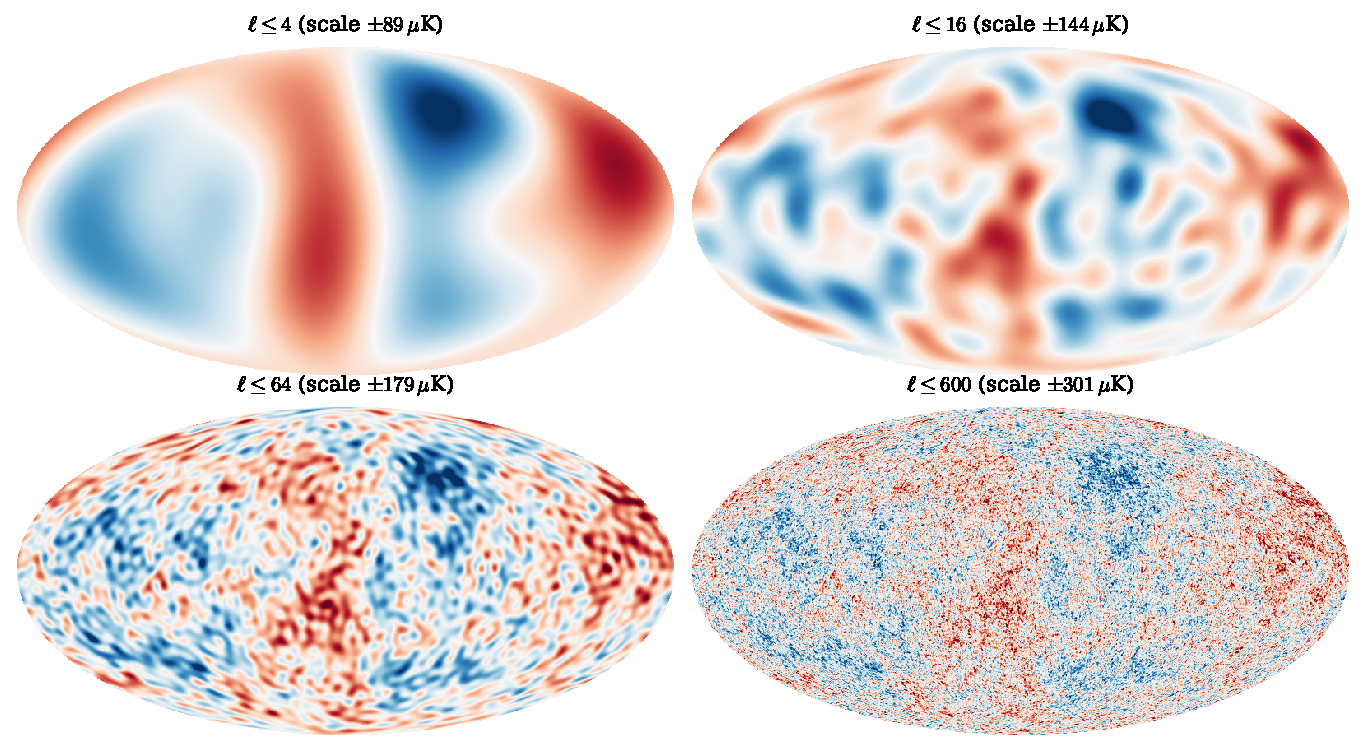
\includegraphics[width=0.95\linewidth]{figures/ch07/truncation.pdf}
\caption{One simulated CMB sky (fiducial $\Lambda$CDM spectrum) summed up to $\ell_{\max}=4$,
$16$, $64$ and $600$. The coefficients are the same in all four panels; each panel simply keeps
more of them. The colour scale is set separately in each panel, because adding multipoles adds
variance. The large-scale pattern of the first panel is still visible underneath the fine
structure of the last.}
\label{7b:fig:truncation}
\end{figure}
\section{No preferred direction: why the $\alm$ are uncorrelated}
\label{7b:sec:isotropy}

A cosmological model does not predict our sky. Inflation predicts the statistics of the
primordial fluctuations, and linear physics carries those statistics forward to the last
scattering surface; the particular pattern of hot and cold spots we see is one draw from that
ensemble of possible skies (\cref{ch:T1}). The property of the ensemble that we rely on most
is that it has no preferred direction: turn the whole sky through any rotation, and the
collection of possible skies, with their probabilities, is unchanged. This does not say that our
sky looks the same in every direction. Our sky may well have a striking feature somewhere; the
statement is that the feature was equally likely to point anywhere.

In flat space the matching symmetry was homogeneity (invariance under shifts), and it made the
Fourier amplitudes of different wavevectors uncorrelated, $\langle\delta_{\bm k}\delta^*_{\bm k'}\rangle
\propto\delta(\bm k-\bm k')P(k)$ (\cref{7a:sec:wk}). The reason was simple: shifting a plane wave
only changes its phase. Rotations of the sphere are harder, because rotations about different
axes do not commute and a general rotation mixes harmonics with different $m$. The tool that
handles this is one we already know, the angular-momentum algebra of quantum mechanics.

\paragraph{The question.} If no direction on the sky is special, which pairs of coefficients
$\alm$, $a_{\ell'm'}$ can be correlated, and can the variance of $\alm$ depend on $m$?

\begin{workdef}[statistical isotropy]
A random sky $\Theta(\bm e)$ is \newterm{statistically isotropic} if for every rotation $R$ the
rotated sky $\Theta(R^{-1}\bm e)$ has the same joint distribution as $\Theta(\bm e)$
\unpack{same probabilities for the temperatures at any finite set of directions}.
For the mean and the two-point function this means
\begin{equation}
  \langle\Theta(\bm e)\rangle=0,\qquad
  \langle\Theta(\bm e)\Theta(\bm e')\rangle=C(\bm e\cdot\bm e'),
  \label{7b:eq:iso-2pt}
\end{equation}
where $C$ is the \newterm{angular correlation function} \unpack{the average product of the
temperatures at two directions, a function of the angle $\vartheta$ between them only, with
$\cos\vartheta=\bm e\cdot\bm e'$} \srcref{HobsonBMC}{(10.1)}. Angle brackets are averages over
the ensemble of skies, never over our one sky.
\end{workdef}

The mean is zero because we subtracted the average temperature; the correlation depends on the
angle alone because a rotation can carry any pair of directions to any other pair with the same
separation.

\subsection{The covariance of two coefficients is a double integral}
\label{7b:sec:cov-integral}

Start from the definition of the coefficients \eqref{7b:eq:alm} and average:
\begin{align}
  \langle\alm\,a^*_{\ell'm'}\rangle
  &\eqby{1}\Bigl\langle\int\dd\Omega\,\Theta(\bm e)Y^*_{\ell m}(\bm e)
     \int\dd\Omega'\,\Theta(\bm e')Y_{\ell'm'}(\bm e')\Bigr\rangle \nonumber\\
  &\eqby{2}\int\dd\Omega\int\dd\Omega'\;\langle\Theta(\bm e)\Theta(\bm e')\rangle\,
     Y^*_{\ell m}(\bm e)\,Y_{\ell'm'}(\bm e') \nonumber\\
  &\eqby{3}\int\dd\Omega\int\dd\Omega'\;C(\bm e\cdot\bm e')\,
     Y^*_{\ell m}(\bm e)\,Y_{\ell'm'}(\bm e') .
  \label{7b:eq:cov-double}
\end{align}
\begin{explain}
  \item Definition \eqref{7b:eq:alm} for both coefficients; conjugating $a_{\ell'm'}$ conjugates
        the harmonic but not the real sky.
  \item The average of a sum (an integral) is the sum of the averages, and the harmonics are
        fixed functions, not random.
  \item Isotropy \eqref{7b:eq:iso-2pt}.
\end{explain}
Since $\langle\alm\rangle=\int\dd\Omega\,\langle\Theta\rangle Y^*_{\ell m}=0$, this average is
the covariance of the two coefficients. The question has become: what does this double integral
give, given that its kernel $C(\bm e\cdot\bm e')$ depends only on the angle between the two
directions? We answer it in two steps. First we use only the rotations about the pole, which
need nothing but the factor $e^{im\phi}$ in each harmonic. Then we use all rotations, which need
the angular-momentum algebra.

\subsection{Rotations about the pole: $m$ must equal $m'$}
\label{7b:sec:z-rotations}

\emph{The question.} What does a rotation about the pole do to the coefficients? Rotate the sky
by an angle $\alpha$ about the $z$-axis. The new sky has, at longitude $\phi$, the temperature
the old sky had at $\phi-\alpha$: $\Theta_\alpha(\theta,\phi)=\Theta(\theta,\phi-\alpha)$.
Its coefficients are
\begin{align}
  a^{(\alpha)}_{\ell m}
  &\eqby{1}\int\dd\Omega\;\Theta(\theta,\phi-\alpha)\,Y^*_{\ell m}(\theta,\phi)
   \eqby{2}\int\dd\Omega'\;\Theta(\theta,\phi')\,Y^*_{\ell m}(\theta,\phi'+\alpha)
   \eqby{3}e^{-im\alpha}\,\alm .
   \label{7b:eq:z-rotation}
\end{align}
\begin{explain}
  \item Definition \eqref{7b:eq:alm} applied to the rotated sky.
  \item Substitute $\phi'=\phi-\alpha$; the solid-angle element and the range of a full turn are
        unchanged.
  \item $Y_{\ell m}\propto e^{im\phi}$, so $Y^*_{\ell m}(\theta,\phi'+\alpha)=e^{-im\alpha}
        Y^*_{\ell m}(\theta,\phi')$.
\end{explain}
So a rotation about the pole only changes the phase of each coefficient, by an angle
proportional to $m$.

\emph{Now use isotropy.} The rotated sky is a draw from the same ensemble, so its coefficients
have the same covariances as the original ones. Hence, for every angle $\alpha$,
\begin{equation}
  \langle\alm a^*_{\ell'm'}\rangle
  =\langle a^{(\alpha)}_{\ell m}a^{(\alpha)*}_{\ell'm'}\rangle
  =e^{-i(m-m')\alpha}\,\langle\alm a^*_{\ell'm'}\rangle .
  \label{7b:eq:m-selection}
\end{equation}
If $m\neq m'$ we can pick $\alpha$ with $e^{-i(m-m')\alpha}\neq1$ (for example
$\alpha=\pi/|m-m'|$, which gives $-1$). Then the covariance equals $-1$ times itself, and the
only such number is zero. So coefficients with different $m$ are uncorrelated. This is the same logic as
momentum conservation: a symmetry under shifts of $\phi$ forbids correlations between different
eigenvalues of the generator of those shifts, $L_z=-i\partial_\phi$.

\paragraph{Example: turning the equatorial dipole.} The dipole $B\sin\theta\cos\phi$ of
\cref{7b:sec:alm} had $a_{11}=-B\sqrt{2\pi/3}$. Rotate it by $\alpha=90^\circ$ about the pole:
the hot spot moves from $\phi=0$ to $\phi=90^\circ$, and the sky becomes $B\sin\theta\sin\phi$.
\Cref{7b:eq:z-rotation} predicts $a_{11}\to e^{-i\pi/2}a_{11}=iB\sqrt{2\pi/3}$. Directly, with
$\sin\phi=(e^{i\phi}-e^{-i\phi})/2i$ and the same table \eqref{7b:eq:ylm-explicit},
\begin{align}
  B\sin\theta\sin\phi
  &\eqby{1}\frac{B}{2i}\bigl(\sin\theta e^{i\phi}-\sin\theta e^{-i\phi}\bigr)
   \eqby{2}\frac{B}{2i}\sqrt{\frac{8\pi}{3}}\bigl(-Y_{11}-Y_{1,-1}\bigr)
   \eqby{3}iB\sqrt{\frac{2\pi}{3}}\,Y_{11}+iB\sqrt{\frac{2\pi}{3}}\,Y_{1,-1},
\end{align}
\begin{explain}
  \item Euler's formula for $\sin\phi$.
  \item $\sin\theta e^{i\phi}=-\sqrt{8\pi/3}\,Y_{11}$ and $\sin\theta e^{-i\phi}=\sqrt{8\pi/3}\,Y_{1,-1}$.
  \item $-1/(2i)=i/2$, and $\tfrac12\sqrt{8\pi/3}=\sqrt{2\pi/3}$.
\end{explain}
so $a_{11}=iB\sqrt{2\pi/3}$, as predicted. Only the phase moved; $|a_{11}|$ did not.

\subsection{All rotations: one $\ell$ at a time, and no dependence on $m$}
\label{7b:sec:all-rotations}

Rotations about other axes mix different $m$, so the phase argument no longer works on its own.
The idea instead is to write the covariance as a matrix element of an operator, and then use
what quantum mechanics tells us about operators that commute with rotations. Define the \newterm{covariance operator} $\hat C$, which acts on a
function $f$ on the sphere by smoothing it with the correlation function,
\begin{equation}
  (\hat Cf)(\bm e)=\int\dd\Omega'\;C(\bm e\cdot\bm e')\,f(\bm e'),
  \label{7b:eq:cov-operator}
\end{equation}
and use the inner product $\braket{f}{g}=\int\dd\Omega\,f^*g$ of wavefunctions on the sphere,
with $\ket{\ell m}$ standing for $Y_{\ell m}$. Then \eqref{7b:eq:cov-double} reads
\begin{equation}
  \langle\alm\,a^*_{\ell'm'}\rangle=\int\dd\Omega\;Y^*_{\ell m}(\bm e)\,(\hat CY_{\ell'm'})(\bm e)
  =\bra{\ell m}\hat C\ket{\ell'm'} .
  \label{7b:eq:cov-matrix-element}
\end{equation}
The covariance matrix of the coefficients is the matrix of $\hat C$ in the basis of spherical
harmonics, exactly as the matrix of a Hamiltonian in the $\ket{\ell m}$ basis.

\paragraph{The covariance operator commutes with every rotation.} Let $U_R$ rotate a function,
$(U_Rf)(\bm e)=f(R^{-1}\bm e)$. Then
\begin{align}
  (U_R\hat Cf)(\bm e)
  &\eqby{1}\int\dd\Omega'\;C\bigl((R^{-1}\bm e)\cdot\bm e'\bigr)\,f(\bm e')
   \eqby{2}\int\dd\Omega''\;C\bigl((R^{-1}\bm e)\cdot(R^{-1}\bm e'')\bigr)\,f(R^{-1}\bm e'')
   \nonumber\\
  &\eqby{3}\int\dd\Omega''\;C(\bm e\cdot\bm e'')\,(U_Rf)(\bm e'')
   \eqby{4}(\hat CU_Rf)(\bm e) .
   \label{7b:eq:commute}
\end{align}
\begin{explain}
  \item Definition of $U_R$ applied to the function $\hat Cf$.
  \item Change variables $\bm e'=R^{-1}\bm e''$; a rotation preserves solid angle, so
        $\dd\Omega'=\dd\Omega''$.
  \item A rotation preserves dot products, $(R^{-1}\bm a)\cdot(R^{-1}\bm b)=\bm a\cdot\bm b$; and
        $f(R^{-1}\bm e'')=(U_Rf)(\bm e'')$.
  \item Definition \eqref{7b:eq:cov-operator}.
\end{explain}
So $U_R\hat C=\hat CU_R$ for every rotation. Now take a rotation by a small angle
$\varepsilon$ about a unit axis $\bm n$. In quantum mechanics the angular momentum is the
generator of rotations, $U_R=1-i\varepsilon\,\bm n\cdot\bm L+O(\varepsilon^2)$. Insert this
into $U_R\hat C=\hat CU_R$: the terms $\hat C$ cancel, and the terms of order $\varepsilon$ give
$(\bm n\cdot\bm L)\hat C=\hat C(\bm n\cdot\bm L)$. Taking $\bm n$ along $x$, $y$ and $z$ in turn,
and then noting that $\bm L^2$ and $L_\pm$ are built from $L_x,L_y,L_z$, we get
\begin{equation}
  [\hat C,L_x]=[\hat C,L_y]=[\hat C,L_z]=0
  \quad\Longrightarrow\quad
  [\hat C,\bm L^2]=0,\qquad [\hat C,L_\pm]=0,
  \label{7b:eq:commutators}
\end{equation}
with the ladder operators $L_\pm=L_x\pm iL_y$. These commutators answer the question in three
short steps.

\paragraph{Step 1: different $\ell$ are uncorrelated.} Sandwich $\hat C\bm L^2=\bm L^2\hat C$
between $\bra{\ell m}$ and $\ket{\ell'm'}$:
\begin{align}
  \ell'(\ell'+1)\bra{\ell m}\hat C\ket{\ell'm'}
  &\eqby{1}\bra{\ell m}\hat C\bm L^2\ket{\ell'm'}
   \eqby{2}\bra{\ell m}\bm L^2\hat C\ket{\ell'm'}
   \eqby{3}\ell(\ell+1)\bra{\ell m}\hat C\ket{\ell'm'} .
\end{align}
\begin{explain}
  \item $\bm L^2\ket{\ell'm'}=\ell'(\ell'+1)\ket{\ell'm'}$ from \eqref{7b:eq:ylm-eigen}.
  \item $\hat C$ commutes with $\bm L^2$ \eqref{7b:eq:commutators}.
  \item $\bm L^2$ is Hermitian, so it acts to the left on $\bra{\ell m}$ with its real
        eigenvalue.
\end{explain}
If $\ell\neq\ell'$ then $\ell(\ell+1)\neq\ell'(\ell'+1)$ and the matrix element vanishes.
\paragraph{Step 2: different $m$ are uncorrelated.} The same sandwich with $L_z$ gives
$(m-m')\bra{\ell m}\hat C\ket{\ell m'}=0$. This is the infinitesimal version of
\eqref{7b:eq:m-selection}.

\paragraph{Step 3: the variance does not depend on $m$.} After steps 1 and 2, only the diagonal
elements $c_m\equiv\bra{\ell m}\hat C\ket{\ell m}=\langle|\alm|^2\rangle$ survive. The question
is whether they can differ from one $m$ to the next. The ladder
operators move between neighbouring $m$ with the real, positive coefficients of quantum mechanics,
$L_+\ket{\ell m}=\lambda_m\ket{\ell,m+1}$ and $L_-\ket{\ell,m+1}=\lambda_m\ket{\ell m}$, where
$\lambda_m=\sqrt{\ell(\ell+1)-m(m+1)}$. Compute one matrix element in two ways:
\begin{align}
  \lambda_m\,c_{m+1}
  &\eqby{1}\bra{\ell,m+1}\hat C\,L_+\ket{\ell m}
   \eqby{2}\bra{\ell,m+1}L_+\hat C\ket{\ell m}
   \eqby{3}\bigl(L_-\ket{\ell,m+1}\bigr)^\dagger\hat C\ket{\ell m}
   \eqby{4}\lambda_m\,c_m .
   \label{7b:eq:ladder}
\end{align}
\begin{explain}
  \item $L_+\ket{\ell m}=\lambda_m\ket{\ell,m+1}$, and the definition of $c_{m+1}$.
  \item $\hat C$ commutes with $L_+$ \eqref{7b:eq:commutators}.
  \item The adjoint of $L_+$ is $L_-$ (because $L_x$ and $L_y$ are Hermitian), so $L_+$ acting
        to the left is $L_-$ acting on the bra's ket.
  \item $L_-\ket{\ell,m+1}=\lambda_m\ket{\ell m}$ with $\lambda_m$ real, and the definition of $c_m$.
\end{explain}
For $m=-\ell,\dots,\ell-1$ the factor $\lambda_m$ is strictly positive (it vanishes only at
$m=\ell$), so we may divide by it: $c_{m+1}=c_m$. Walking from $m=-\ell$ up to $m=\ell$, all
$2\ell+1$ diagonal elements are equal. Call their common value $\Cell$.

\begin{keyidea}[Isotropy diagonalises the sky]
For a statistically isotropic sky,
\begin{equation}
  \langle\alm\rangle=0,\qquad
  \langle\alm\,a^*_{\ell'm'}\rangle=\Cell\,\delta_{\ell\ell'}\,\delta_{mm'} .
  \label{7b:eq:alm-cov}
\end{equation}
The \newterm{angular power spectrum} $\Cell$ is the variance of each coefficient at multipole
$\ell$, the same for all $2\ell+1$ values of $m$
\srcref{HobsonBMC}{(10.3)}, \srcref{Hivon}{(7)}.
\end{keyidea}

In group-theory language this is Schur's lemma: the harmonics with a given $\ell$ carry an
irreducible representation of the rotation group, and an operator that commutes with an
irreducible representation is a multiple of the identity on it. The ladder-operator argument
above is the proof of that lemma in the one case we need. The result also shows that $\Cell$ is
\emph{all} an isotropic two-point function can contain: one number per $\ell$.

The result also fixes the average of a product without a conjugate. The reality condition
\eqref{7b:eq:reality}, read with $m\to-m'$, says $a_{\ell'm'}=(-1)^{m'}a^*_{\ell',-m'}$. Insert this
and use \eqref{7b:eq:alm-cov}: $\langle\alm a_{\ell'm'}\rangle=(-1)^{m'}\langle\alm
a^*_{\ell',-m'}\rangle=(-1)^m\Cell\,\delta_{\ell\ell'}\delta_{m,-m'}$. In particular
$\langle\alm^2\rangle=0$ whenever $m\neq0$, a fact that fixes the distribution of the real and
imaginary parts in \cref{7b:sec:chat}.

\begin{pitfall}[Isotropy is a property of the ensemble, not of our sky]
Every single sky has directions that stand out: the $\ell\le4$ panel of
\cref{7b:fig:truncation} has a hot band and two cold blobs. Isotropy says that a rotated version
of that sky was exactly as likely, not that the sky looks the same in all directions. The
$\alm$ of one sky are what they are; the statement \eqref{7b:eq:alm-cov} is about their averages
over many hypothetical skies.
\end{pitfall}

\subsection{From $\Cell$ back to the correlation function}
\label{7b:sec:ctheta}

The correlation function $C(\vartheta)$ of \eqref{7b:eq:iso-2pt} and the power spectrum $\Cell$
carry the same information: each is a Legendre series of the other. To show it we need the \newterm{addition theorem} for spherical harmonics, the sphere's
version of $\sum_{\bm k}e^{i\bm k\cdot(\bm x-\bm x')}$ depending only on $\bm x-\bm x'$:
\begin{equation}
  \sum_{m=-\ell}^{\ell}Y_{\ell m}(\bm e)\,Y^*_{\ell m}(\bm e')=\frac{2\ell+1}{4\pi}\,
  P_\ell(\bm e\cdot\bm e'),
  \label{7b:eq:addition}
\end{equation}
with $P_\ell$ the Legendre polynomial ($P_0=1$, $P_1(x)=x$, $P_2(x)=(3x^2-1)/2$). Check it for
$\ell=1$ with both directions at the north pole: only $m=0$ survives at $\theta=0$, and
$|Y_{10}|^2=3/4\pi=(3/4\pi)P_1(1)$. Then
\begin{align}
  C(\bm e\cdot\bm e')=\langle\Theta(\bm e)\Theta(\bm e')\rangle
  &\eqby{1}\sum_{\ell m}\sum_{\ell'm'}\langle\alm a^*_{\ell'm'}\rangle\,Y_{\ell m}(\bm e)\,Y^*_{\ell'm'}(\bm e')
   \nonumber\\
  &\eqby{2}\sum_{\ell}\Cell\sum_{m=-\ell}^{\ell}Y_{\ell m}(\bm e)\,Y^*_{\ell m}(\bm e')
   \eqby{3}\sum_{\ell}\frac{2\ell+1}{4\pi}\,\Cell\,P_\ell(\cos\vartheta) .
   \label{7b:eq:ctheta}
\end{align}
\begin{explain}
  \item Expand $\Theta(\bm e)$ in $Y_{\ell m}$ and the real $\Theta(\bm e')=\Theta^*(\bm e')$ in
        $Y^*_{\ell'm'}$, and average term by term.
  \item \Cref{7b:eq:alm-cov} keeps $\ell=\ell'$, $m=m'$.
  \item Addition theorem \eqref{7b:eq:addition}, with $\cos\vartheta=\bm e\cdot\bm e'$.
\end{explain}
This is \srcref{HobsonBMC}{(10.4)}. To invert it, multiply by $P_{\ell'}(\cos\vartheta)$ and integrate over $x=\cos\vartheta$, using
$\int_{-1}^1P_\ell P_{\ell'}\,\dd x=2\delta_{\ell\ell'}/(2\ell+1)$:
\begin{equation}
  \Cell=2\pi\int_{-1}^{1}\dd(\cos\vartheta)\;P_\ell(\cos\vartheta)\,C(\vartheta) .
  \label{7b:eq:ctheta-inverse}
\end{equation}
(Hobson et al.\ print the prefactor as $4\pi$ \srcref{HobsonBMC}{(10.5)}; the orthogonality
integral above gives $2\pi$.)\footnote{Insert \eqref{7b:eq:ctheta} into the right-hand side:
$2\pi\sum_{\ell'}\frac{2\ell'+1}{4\pi}C_{\ell'}\cdot\frac{2\delta_{\ell\ell'}}{2\ell+1}=\Cell$. With
$4\pi$ the right-hand side would be $2\Cell$.}

How much does each multipole add to the temperature variance at one point? At zero
separation, $P_\ell(1)=1$, and the correlation function is that variance,
\begin{equation}
  \sigma_\Theta^2=C(0)=\sum_\ell\frac{2\ell+1}{4\pi}\,\Cell .
  \label{7b:eq:var-point}
\end{equation}
Each multipole contributes $(2\ell+1)\Cell/4\pi$: the factor $2\ell+1$ counts the patterns at
that $\ell$ and $\Cell$ is the variance of each. Per logarithmic interval of $\ell$ the
contribution is $\ell(2\ell+1)\Cell/4\pi\approx\ell(\ell+1)\Cell/2\pi=D_\ell$, which is why $D_\ell$
is the quantity that is plotted (\cref{ch:T1}).

\paragraph{The covariance of a map.} In pixels the covariance is a full matrix; in harmonics
it is diagonal. A map is the sky sampled at pixel centres $\bm e_p$, usually smoothed by the
telescope beam. A circular beam multiplies each $\alm$ by a number $B_\ell$ (its harmonic
transform), so $\Cell\to\Cell B_\ell^2$; this is the sphere's version of smoothing in flat space
(\cref{7a:sec:smoothing}). The signal in two pixels $p$ and $p'$ then has the covariance
\begin{equation}
  \bm C^{S}_{pp'}=\sum_{\ell}\frac{2\ell+1}{4\pi}\,\Cell B_\ell^2\,P_\ell(\cos\vartheta_{pp'}),
  \label{7b:eq:pixel-cov}
\end{equation}
which is \eqref{7b:eq:ctheta} with the beam included and $\vartheta_{pp'}$ the angle between the
two pixel centres \srcref{HobsonBMC}{(10.18)}. This $N_{\rm pix}\times N_{\rm pix}$ matrix is the
signal covariance of a Gaussian likelihood written in pixels. Every entry is nonzero, since any
two pixels are correlated. In harmonic space the same covariance \eqref{7b:eq:alm-cov} is
diagonal. That is why we work with the $\alm$.

\paragraph{Example: the rms of the CMB.} For the fiducial spectrum (\cref{7b:sec:camb}),
\pyname{code/ch07/}\allowbreak\pyname{22_isotropy.py} evaluates \eqref{7b:eq:var-point} up to $\ell=2000$:
$\sigma_\Theta^2=\SBvarZero\,\mu\mathrm K^2$, an rms of $\SBrmsZero\,\mu$K, the ``hundred
microkelvin'' of the opening paragraph. The multipoles $\ell\le30$ supply $\SBfracLowL\%$ of
this variance, although they are only about $10^3$ of the four million coefficients up to
$\ell=2000$. \Cref{7b:fig:ctheta}(a) shows how fast the correlation falls: by a separation of
one degree, $C(\vartheta)$ has dropped to about a quarter of its value at zero, which is the
statement that most of the variance sits in features smaller than about a degree, the scale of
the first acoustic peak.

\Cref{7b:fig:ctheta}(b) makes a point that matters for statistics: the correlation function
measured on one sky can differ from the ensemble prediction by as much as the prediction itself,
at large separations. What we measure on one sky is the average of $\Theta(\bm e)\Theta(\bm e')$
over all pairs of directions at separation $\vartheta$. This equals the same Legendre series
\eqref{7b:eq:ctheta} with $\Cell$ replaced by that sky's own average over $m$,
$\Chat=\sum_m|\alm|^2/(2\ell+1)$. (Averaging the pair over all orientations does to the product
of harmonics what the ensemble average did in step (2) of \eqref{7b:eq:ctheta}.) Five
simulated skies give five visibly different curves at large separations. They scatter around the
ensemble prediction by $80$ to $180\,\mu\mathrm K^2$ at $30^\circ$ to $90^\circ$, which is as large as
the signal itself there ($|C|\approx160$ to $230\,\mu\mathrm K^2$). This is cosmic variance
seen in real space. It is large at large $\vartheta$ because large separations are controlled
by the few low multipoles, and a low multipole has few coefficients to average over. We
quantify it in \cref{7b:sec:chat}.

\begin{figure}[htbp]
\centering
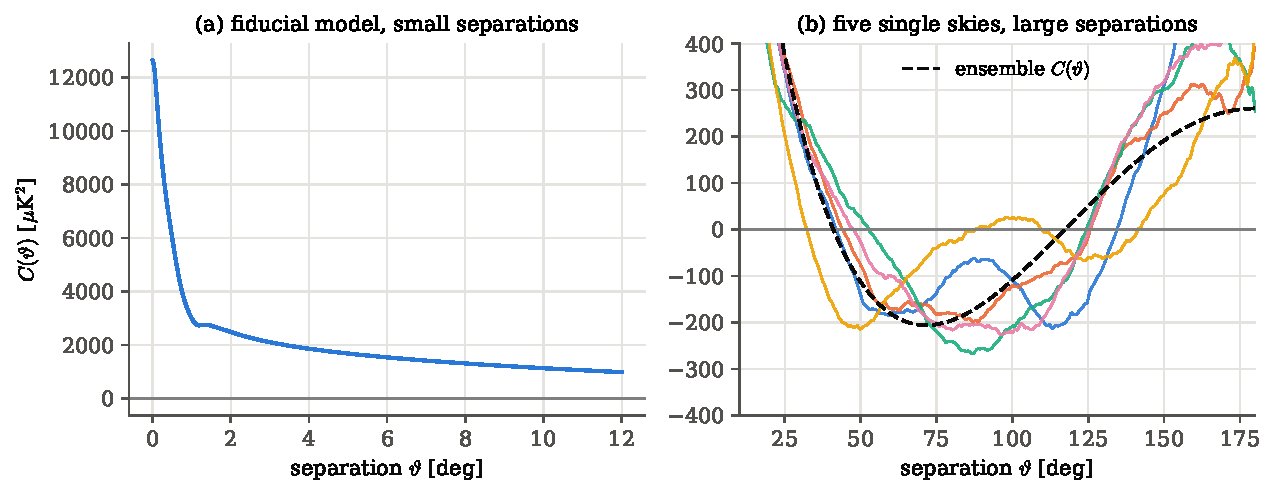
\includegraphics[width=0.98\linewidth]{figures/ch07/ctheta.pdf}
\caption{(a) The angular correlation function of the fiducial model for separations up to
$12^\circ$. It falls from the point variance $C(0)\approx1.3\times10^4\,\mu$K$^2$ to a quarter of
that within one degree, then decays slowly. (b) Large separations: the ensemble $C(\vartheta)$
(black dashed) and the full-sky pair average for five single simulated skies (coloured). The
five skies are drawn from the same model; their differences are cosmic variance.}
\label{7b:fig:ctheta}
\end{figure}

\subsection{Seeing isotropy, and its violation, in simulated skies}
\label{7b:sec:iso-test}

The argument of \cref{7b:sec:all-rotations} makes two predictions we can test: within one
$\ell$, the average power $\langle|\alm|^2\rangle$ is the same for every $m$; and different $\ell$
are uncorrelated. A test is convincing only if it can fail, so we also build a sky that is
\emph{not} isotropic and check that both predictions break.

\paragraph{Example: a sky with a preferred axis.} Multiply an isotropic sky by
$1+A\cos\theta$. Fluctuations are then amplified by a factor $1+A$ at the north pole and damped
by $1-A$ at the south pole: the $z$-axis is special. (A small effect of this kind, a
``hemispherical power asymmetry'', is one of the anomalies that the Planck collaboration tests
for \cite{Planck2018VII}.) What does the modulation do to the coefficients? In harmonic space,
multiplying by $\cos\theta$ is simple, because $\cos\theta\propto Y_{10}$ carries one unit of
angular momentum along $z$. It changes $\ell$ by $\pm1$ and keeps $m$, the dipole selection rule
of atomic physics:
\begin{equation}
  \cos\theta\;Y_{\ell m}=c_{\ell+1,m}\,Y_{\ell+1,m}+c_{\ell m}\,Y_{\ell-1,m},\qquad
  c_{\ell m}=\sqrt{\frac{\ell^2-m^2}{(2\ell+1)(2\ell-1)}} .
  \label{7b:eq:cos-recursion}
\end{equation}
Check it on $\ell=0$: $\cos\theta\,Y_{00}=\cos\theta/\sqrt{4\pi}=\sqrt{1/3}\,Y_{10}$, and
$c_{10}=\sqrt{1/3}$. The coefficients of the modulated sky $\Theta'=(1+A\cos\theta)\Theta$ are
\begin{align}
  a'_{LM}
  &\eqby{1}a_{LM}+A\sum_{\ell m}\alm\int\dd\Omega\;\cos\theta\,Y_{\ell m}Y^*_{LM}
   \eqby{2}a_{LM}+A\bigl(c_{LM}\,a_{L-1,M}+c_{L+1,M}\,a_{L+1,M}\bigr) .
   \label{7b:eq:modulated}
\end{align}
\begin{explain}
  \item Definition \eqref{7b:eq:alm} for $\Theta'$, with $\Theta$ expanded in harmonics.
  \item \Cref{7b:eq:cos-recursion} and orthonormality: the term $Y_{\ell+1,m}$ contributes when
        $\ell+1=L$, the term $Y_{\ell-1,m}$ when $\ell-1=L$, and only for $m=M$.
\end{explain}
Each new coefficient is a mix of three old ones, which are independent. Averaging products
with \eqref{7b:eq:alm-cov} for the old sky gives
\begin{align}
  \langle a'_{\ell+1,m}\,a'^*_{\ell m}\rangle&=A\,c_{\ell+1,m}\,(\Cell+C_{\ell+1}),
  \label{7b:eq:mod-cross}\\
  \langle|a'_{\ell m}|^2\rangle&=\Cell+A^2\bigl(c_{\ell m}^2\,C_{\ell-1}+c_{\ell+1,m}^2\,C_{\ell+1}\bigr).
  \label{7b:eq:mod-power}
\end{align}
Both predictions of isotropy now fail. By \eqref{7b:eq:mod-cross}, neighbouring multipoles are
correlated. By \eqref{7b:eq:mod-power}, the power depends on $m$ through $c_{\ell m}^2$ and
$c_{\ell+1,m}^2$, which are both largest at $m=0$ and shrink towards $|m|=\ell$ (where $c_{\ell m}$
vanishes). Both violations come from the preferred axis.

The script \pyname{code/ch07/22_isotropy.py} draws $\SBisoNsim$ isotropic skies up to
$\ell=42$ from the fiducial spectrum, modulates each one with $A=\SBisoAmp$ using
\eqref{7b:eq:modulated}, and averages. The modulation is done exactly in harmonic space by the
function \pyname{modulate_dipole} of the small library \pyname{code/ch07/lib_harmonic.py}:
\pyfile[firstline=84,lastline=96,firstnumber=84]{code/ch07/lib_harmonic.py}{Multiplying a sky by $1+A\cos\theta$, coefficient by coefficient}
\noindent Lines 91--92 find which neighbours $a_{L\mp1,M}$ exist (the stored list starts at
$\ell=m$ and stops at $\ell_{\max}$); lines 94--95 add the two terms of
\eqref{7b:eq:modulated}. In the storage order of healpy, which the library uses (\cref{7b:sec:healpix}),
$a_{L-1,M}$ and $a_{L+1,M}$ sit just before and just after $a_{LM}$.

\Cref{7b:fig:isotropy-test} shows the result at $\ell=20$. For the isotropic skies the power is
the same in every $m$: the largest deviation of $\langle|a_{20,m}|^2\rangle/C_{20}$ from $1$ among
$m=1,\dots,20$ is $\SBisoPowDevMax$, about two standard errors of $\SBisoErr$ (since
$|\alm|^2/\Cell$ has standard deviation $1$ for $m>0$, as we will see), which is what the largest of
twenty independent deviations typically is. The correlation between $\ell=20$ and $\ell=21$ is
zero within $\SBisoXmax$. For the modulated skies both predictions fail exactly as
\eqref{7b:eq:mod-cross} and \eqref{7b:eq:mod-power} say: the power rises to $\SBmodPowZero\,C_{20}$
at $m=0$, and the neighbour correlation reaches $\SBmodXzero\,C_{20}$ at $m=0$ and falls towards
$|m|=\ell$.

\begin{figure}[htbp]
\centering
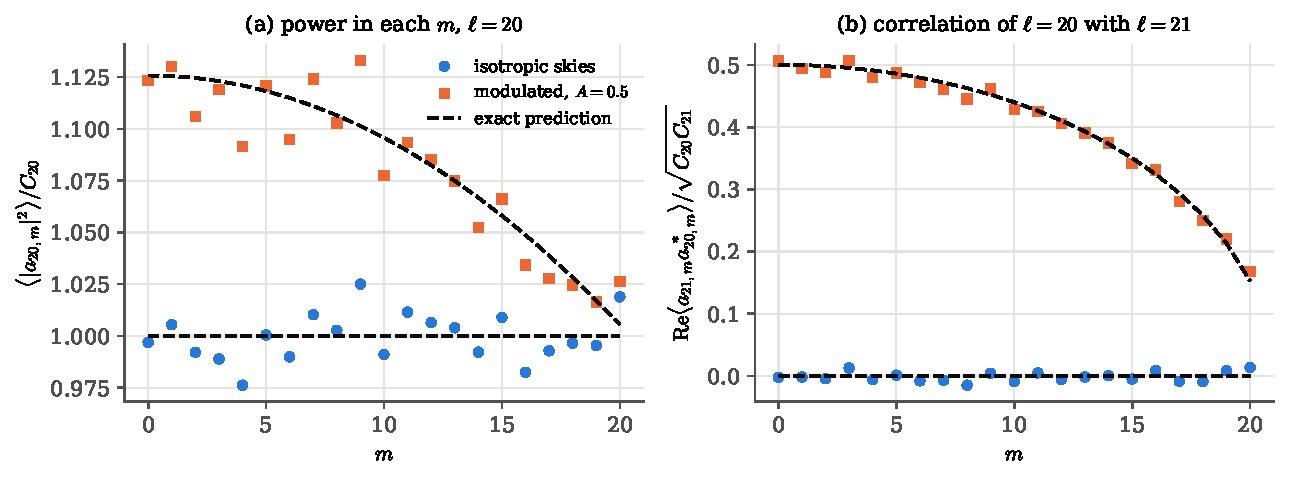
\includegraphics[width=0.98\linewidth]{figures/ch07/isotropy_test.pdf}
\caption{Two predictions of isotropy, tested on $\SBisoNsim$ simulated skies at $\ell=20$. (a)
Average power in each $m$, in units of $C_{20}$: flat for isotropic skies (blue), tilted for
skies modulated by $1+0.5\cos\theta$ (orange). (b) Average product of the coefficients at
$\ell=21$ and $\ell=20$ with the same $m$: zero for isotropic skies, large for modulated ones.
Black dashed lines are the exact predictions \eqref{7b:eq:mod-cross} and
\eqref{7b:eq:mod-power} (and $1$, $0$ for the isotropic case).}
\label{7b:fig:isotropy-test}
\end{figure}

\paragraph{Gaussianity turns ``uncorrelated'' into ``independent''.} So far isotropy has told us
which coefficients are uncorrelated. For a Gaussian sky that is enough to make them independent.
The coefficients are integrals of the sky with fixed weights, so they are linear combinations of
the field values. If
the field is Gaussian (as linear evolution of Gaussian initial conditions guarantees,
\srcref{HobsonBMC}{p.~230}), the coefficients are jointly Gaussian, and for jointly Gaussian
variables zero correlation means independence (\cref{ch:02}). For complex coefficients we must
be careful about what ``zero correlation'' means, since a complex number is two real numbers;
\cref{7b:sec:chat} does that bookkeeping and turns \eqref{7b:eq:alm-cov} into the exact
distribution of the power-spectrum estimator.
\section{One sky, $2\ell+1$ numbers: the estimator $\Chat$ and cosmic variance}
\label{7b:sec:chat}

The model predicts $\Cell=\langle|\alm|^2\rangle$, an average over an ensemble of skies we will
never see. We have one sky. What saves us is the result of \cref{7b:sec:isotropy}: in an
isotropic sky the coefficients at one multipole are uncorrelated and all have the same variance
$\Cell$ \eqref{7b:eq:alm-cov}. So at each multipole the sky hands us $2\ell+1$ real numbers
(the count \eqref{7b:eq:count}) with a common variance. That is the situation of a laboratory
physicist who has measured the same noisy quantity $2\ell+1$ times and wants its variance:
average the squares (the mean is known to be zero). Replacing the ensemble average by this
average over the sphere is called the ergodic replacement. Its
weakness is at low $\ell$, where there are very few numbers to average. That limit comes from
the Universe, not from the instrument.

\paragraph{The question.} If we estimate $\Cell$ by averaging $|\alm|^2$ over the $2\ell+1$
values of $m$, is the estimate right on average, how is it distributed, and how large is its
scatter around the truth?

\begin{workdef}[full-sky power-spectrum estimator]
For a full, noiseless sky,
\begin{equation}
  \Chat=\frac{1}{2\ell+1}\sum_{m=-\ell}^{\ell}|\alm|^2
  =\frac{1}{2\ell+1}\Bigl(a_{\ell0}^2+2\sum_{m=1}^{\ell}|\alm|^2\Bigr)
  \label{7b:eq:chat}
\end{equation}
\unpack{the mean square of the $2\ell+1$ coefficients at one $\ell$, each $m>0$ counted twice
because $|a_{\ell,-m}|=|\alm|$} \srcref{Hivon}{(8)}, \srcref{HobsonBMC}{(10.25)}. healpy's
\pyname{alm2cl} computes exactly this from the stored $m\ge0$ coefficients.
\end{workdef}

The second form uses the reality condition \eqref{7b:eq:reality}, $|a_{\ell,-m}|=|\alm|$. Its
expectation follows in one line from \eqref{7b:eq:alm-cov}:
\begin{equation}
  \E\Chat=\frac{1}{2\ell+1}\sum_{m=-\ell}^{\ell}\langle|\alm|^2\rangle
  =\frac{1}{2\ell+1}\,(2\ell+1)\,\Cell=\Cell .
  \label{7b:eq:chat-unbiased}
\end{equation}
So $\Chat$ is unbiased. Here is the estimator written out from scratch, as every
simulation script in this chapter uses it:
\pyfile[firstline=48,lastline=56,firstnumber=48]{code/ch07/lib_harmonic.py}{The full-sky estimator \eqref{7b:eq:chat} from the stored coefficients}
\noindent Line 54 gives weight $1$ to $m=0$ and weight $2$ to $m>0$, which folds in the negative
$m$ that are not stored. Line 55 adds up the weighted $|\alm|^2$ for each $\ell$ with
\pyname{np.bincount}, and line 56 divides by $2\ell+1$. Applied to the same coefficients, it
agrees with healpy's \pyname{alm2cl} to a relative $\SBourVsHp$, rounding error.

\subsection{Counting real degrees of freedom}
\label{7b:sec:dof}

$\Chat$ is a sum of squares. To find its distribution we need the distribution of the real
numbers being squared, the real and imaginary parts of the $\alm$. Fix $\ell$ and write $\alm=x_m+iy_m$ for $m=1,\dots,\ell$, with $x_m$ and $y_m$ real.
Section~\ref{7b:sec:isotropy} gave us two averages: $\langle\alm a^*_{\ell m}\rangle=\Cell$, and
$\langle\alm^2\rangle=0$ for $m\neq0$. Expand both in real and imaginary parts:
\begin{align}
  \Cell&\eqby{1}\langle|\alm|^2\rangle=\langle x_m^2\rangle+\langle y_m^2\rangle,
  \nonumber\\
  0&\eqby{2}\langle\alm^2\rangle=\langle x_m^2\rangle-\langle y_m^2\rangle+2i\,\langle x_my_m\rangle
  \quad\Longrightarrow\quad
  \langle x_m^2\rangle=\langle y_m^2\rangle=\frac{\Cell}{2},\qquad\langle x_my_m\rangle=0 .
  \label{7b:eq:reim}
\end{align}
\begin{explain}
  \item \Cref{7b:eq:alm-cov} with $\ell'=\ell$, $m'=m$, and $|x+iy|^2=x^2+y^2$.
  \item $\langle\alm a_{\ell'm'}\rangle=(-1)^m\Cell\delta_{\ell\ell'}\delta_{m,-m'}$ vanishes for
        $m'=m\neq0$. The real part of the zero gives $\langle x^2\rangle=\langle y^2\rangle$, the
        imaginary part gives $\langle xy\rangle=0$; with the first line, each is $\Cell/2$.
\end{explain}
What about two different coefficients, $m\neq m'$ with both positive? Both averages vanish:
$\langle\alm a^*_{\ell m'}\rangle=0$ because $m\neq m'$, and $\langle\alm a_{\ell m'}\rangle=0$
because $m'\neq-m$. Taking the real and imaginary parts of these two zeros makes all four
products $\langle x_mx_{m'}\rangle$, $\langle y_my_{m'}\rangle$, $\langle x_my_{m'}\rangle$,
$\langle y_mx_{m'}\rangle$ zero. The same argument with $m'=0$ shows that $a_{\ell0}$ is
uncorrelated with every $x_m$ and $y_m$. Finally, $a_{\ell0}$ is real with
$\langle a_{\ell0}^2\rangle=\Cell$. In summary, at each $\ell$:
\begin{center}
\begin{tabular}{@{}lll@{}}
\toprule
real number & how many & variance\\\midrule
$a_{\ell0}$ & $1$ & $\Cell$\\
$x_m=\mathrm{Re}\,\alm$, $m=1,\dots,\ell$ & $\ell$ & $\Cell/2$\\
$y_m=\mathrm{Im}\,\alm$, $m=1,\dots,\ell$ & $\ell$ & $\Cell/2$\\
$\alm$ with $m<0$ & -- & fixed by $a_{\ell,-m}=(-1)^m\alm^*$\\
\bottomrule
\end{tabular}
\end{center}
For a Gaussian sky these $2\ell+1$ real numbers are jointly Gaussian and uncorrelated, hence
independent (\cref{ch:02}). \Cref{7b:fig:dof} draws the bookkeeping for $\ell=3$.

\begin{figure}[htbp]
\centering
\begin{tikzpicture}[x=1.55cm,y=1cm,font=\small]
  \foreach \m in {-3,-2,-1} {
    \draw[softgray,dashed,fill=black!3] (\m-0.42,0) rectangle (\m+0.42,1.2);
    \node[softgray] at (\m,0.6) {fixed};
    \node[anchor=north] at (\m,-0.05) {$m=\m$};
  }
  \draw[fibreorange,thick,fill=fibreorange!12] (-0.42,0) rectangle (0.42,1.2);
  \fill[fibreorange] (0,0.6) circle (2.6pt);
  \node[anchor=north] at (0,-0.05) {$m=0$};
  \foreach \m in {1,2,3} {
    \draw[formblue,thick,fill=formblue!10] (\m-0.42,0) rectangle (\m+0.42,1.2);
    \fill[formblue] (\m-0.17,0.6) circle (2.6pt);
    \fill[formblue] (\m+0.17,0.6) circle (2.6pt);
    \node[formblue,font=\scriptsize] at (\m-0.17,0.98) {Re};
    \node[formblue,font=\scriptsize] at (\m+0.17,0.98) {Im};
    \node[anchor=north] at (\m,-0.05) {$m=\m$};
  }
  \foreach \m/\h in {1/1.75,2/2.25,3/2.75} {
    \draw[->,softgray,thick] (\m,1.25) .. controls (\m,\h) and (-\m,\h) .. (-\m,1.25);
  }
  \draw[decorate,decoration={brace,amplitude=6pt,mirror}] (-0.42,-0.55) -- (3.42,-0.55);
  \node[anchor=north,align=center] at (1.5,-0.8)
     {$1+2\times3=7=2\ell+1$ independent real Gaussians};
  \node[anchor=west,align=left,font=\scriptsize] at (3.6,0.95)
     {\textcolor{fibreorange}{$\bullet$} variance $\Cell$};
  \node[anchor=west,align=left,font=\scriptsize] at (3.6,0.45)
     {\textcolor{formblue}{$\bullet$} variance $\Cell/2$};
\end{tikzpicture}
\caption{The real degrees of freedom at $\ell=3$. The coefficient with $m=0$ is one real number
of variance $\Cell$ (orange). Each $m>0$ coefficient is two real numbers, its real and imaginary
parts, each of variance $\Cell/2$ (blue). The grey arcs send each $m>0$ cell to its partner
$-m$, which the reality condition fixes completely, so the negative-$m$ cells add nothing new.}
\label{7b:fig:dof}
\end{figure}

Now standardise each real number to unit variance, $z_0=a_{\ell0}/\sqrt{\Cell}$,
$z^{\rm R}_m=x_m/\sqrt{\Cell/2}$, $z^{\rm I}_m=y_m/\sqrt{\Cell/2}$, all independent $\Normal(0,1)$,
and rewrite the estimator:
\begin{align}
  \frac{(2\ell+1)\Chat}{\Cell}
  &\eqby{1}\frac{1}{\Cell}\Bigl(a_{\ell0}^2+2\sum_{m=1}^{\ell}(x_m^2+y_m^2)\Bigr)
   \eqby{2}z_0^2+\frac{2}{\Cell}\,\frac{\Cell}{2}\sum_{m=1}^{\ell}\bigl[(z^{\rm R}_m)^2+(z^{\rm I}_m)^2\bigr]
   \nonumber\\
  &\eqby{3}z_0^2+\sum_{m=1}^{\ell}\bigl[(z^{\rm R}_m)^2+(z^{\rm I}_m)^2\bigr]
   \;\sim\;\chi^2_{2\ell+1} .
   \label{7b:eq:chi2}
\end{align}
\begin{explain}
  \item \Cref{7b:eq:chat} multiplied by $(2\ell+1)/\Cell$, with $|\alm|^2=x_m^2+y_m^2$.
  \item Substitute $a_{\ell0}=\sqrt{\Cell}\,z_0$, $x_m=\sqrt{\Cell/2}\,z^{\rm R}_m$,
        $y_m=\sqrt{\Cell/2}\,z^{\rm I}_m$.
  \item The factor $2$ from the folded negative $m$ cancels the $1/2$ in the variance. What
        remains is a sum of $1+2\ell$ squares of independent standard normals, which is the
        definition of a $\chi^2$ variable with $2\ell+1$ degrees of freedom (\cref{ch:02}).
\end{explain}
Step (3) is why the careful count matters: the factor $2$ from folding and the halved variance
cancel exactly, so every real degree of freedom enters with weight one.

\begin{pitfall}[Two ways to get the count wrong]
(i) Treating all $2\ell+1$ coefficients as independent complex Gaussians gives $2(2\ell+1)$ real
degrees of freedom and a cosmic variance half the true value: it forgets that $a_{\ell,-m}$
is a copy of $\alm$. (ii) Giving the real and imaginary parts of an $m>0$ coefficient the
variance $\Cell$ each doubles $\langle|\alm|^2\rangle$. The one-point density
$p(\alm)=e^{-\alm^2/2\Cell}/\sqrt{2\pi\Cell}$ of and
\srcref{HobsonBMC}{(10.17)} is the density of a \emph{real} variable of variance $\Cell$: exact
for $a_{\ell0}$; for $m>0$ it has to be read as the joint density of $x_m$ and $y_m$, each of
variance $\Cell/2$. Either way the count is $2\ell+1$, and so is the $\chi^2$.
\end{pitfall}

\subsection{The distribution of $\Chat$ and cosmic variance}
\label{7b:sec:cosmic-variance}

We now know that $\Chat$ is a rescaled $\chi^2$ variable. Its density and its scatter follow
from those of $\chi^2$. Write $\nu=2\ell+1$ and $V=\nu\Chat/\Cell\sim\chi^2_\nu$, whose density is
$f_\nu(v)=v^{\nu/2-1}e^{-v/2}/\bigl(2^{\nu/2}\Gamma(\nu/2)\bigr)$ for $v>0$. Since $\Chat=\Cell V/\nu$
is a rescaling, the change-of-variables rule gives the density of the estimator,
\begin{equation}
  p\bigl(\Chat\given\Cell\bigr)=\frac{\nu}{\Cell}\,f_\nu\Bigl(\frac{\nu\Chat}{\Cell}\Bigr),
  \label{7b:eq:chat-pdf}
\end{equation}
a \emph{scaled} $\chi^2_\nu$. Its first two moments
follow from those of $\chi^2_\nu$, which is a Gamma$(\nu/2,2)$ variable with mean $\nu$ and
variance $2\nu$ (\cref{ch:02}):
\begin{align}
  \Var\Chat
  &\eqby{1}\Bigl(\frac{\Cell}{\nu}\Bigr)^2\Var V
   \eqby{2}\frac{\Cell^2}{\nu^2}\,2\nu
   =\frac{2\Cell^2}{2\ell+1} .
   \label{7b:eq:cosmic-var}
\end{align}
\begin{explain}
  \item $\Var(cV)=c^2\Var V$ with $c=\Cell/\nu$.
  \item $\Var\chi^2_\nu=2\nu$.
\end{explain}

\begin{keyidea}[Cosmic variance]
From one full, noiseless sky the power spectrum is measured with
\begin{equation}
  \frac{\Delta\Cell}{\Cell}\equiv\frac{\sqrt{\Var\Chat}}{\Cell}=\sqrt{\frac{2}{2\ell+1}} ,
  \label{7b:eq:cv-frac}
\end{equation}
the sampling error of a variance estimated from $2\ell+1$ Gaussian numbers. No instrument can
reduce it; only more independent modes can. \Cref{ch:03} showed (in the section that finds an
estimator from a model) that $\Chat$ is sufficient for $\Cell$, is its maximum-likelihood
estimator, and attains the Cram\'er--Rao bound, which equals \eqref{7b:eq:cosmic-var}: no unbiased
estimator built from one sky does better.
\end{keyidea}

Hivon et al.\ state the result in one sentence, ``$C_\ell$-s are $\chi^2_\nu$-distributed with the
mean equal to $C^{\rm th}_\ell$, $\nu=2\ell+1$ degrees of freedom, and a variance of
$2{C^{\rm th}_\ell}^2/\nu$'' \srcref{Hivon}{p.~3}.\footnote{Read literally, a $\chi^2_\nu$ variable
has mean $\nu$ and variance $2\nu$. What is meant is the scaled $\chi^2$ of
\eqref{7b:eq:chat-pdf}: $\nu\Chat/\Cell\sim\chi^2_\nu$.} Knox gives the same number as the
noiseless limit of his error formula \cite[eq.~4]{Knox1995}, with the same reading: for each
$\ell$ there are $2\ell+1$ ``samples'' from a Gaussian of variance $\Cell$, and the sampling
variance of a variance is twice its square divided by the number of samples. On the full sky
this sampling variance is called \newterm{cosmic variance}.

The shape matters as much as the width. A $\chi^2_\nu$ has skewness $\sqrt{8/\nu}$ and its mode
sits at $\nu-2$, below the mean $\nu$. So at low $\ell$ the estimator is more often below
$\Cell$ than above it, and occasionally far above. \Cref{7b:fig:chat-pdf}(a) shows the density
\eqref{7b:eq:chat-pdf} in units of $\Cell$ for $\ell=2$, $5$, $20$ and $100$. At $\ell=2$ the
density starts at zero, peaks at $0.6\,\Cell$, and has a long tail; by $\ell=100$ it is a narrow,
nearly symmetric bell, close to the Gaussian of the same mean and variance (dotted lines, shown
for $\ell=5$ and $\ell=100$).

\paragraph{Example: the quadrupole.} At $\ell=2$, $\nu=5$, and \eqref{7b:eq:cv-frac} gives a
fractional error of $\SBfracTwo$: one sky determines the quadrupole only to $63\%$. The
distribution is skewed (skewness $\SBskewTwo$), and the script \pyname{code/ch07/23_cl_distribution.py}
evaluates $\Prob(\widehat C_2<C_2)=\Prob(\chi^2_5<5)=\SBpBelowMean$: a low quadrupole is more
likely than a high one. Suppose the measured quadrupole were a fifth of the model's. In the
language of \cref{ch:04}: if the model were true, would getting a quadrupole this low, or even
lower, be something we'd reasonably expect? The probability is
$\Prob(\widehat C_2<0.2\,C_2)=\Prob(\chi^2_5<1)=\SBpFifth$: small but not negligible. It is even
less alarming than it looks, because the quadrupole was singled out for testing only after the
sky had been seen; with many multipoles to look at, one of them is likely to look odd. A low
quadrupole in the real sky is one of the large-angle features examined in the Planck isotropy
analysis \cite{Planck2018VII}, and this $\chi^2_5$ tail is the first thing any such test computes.

\paragraph{Example: $\ell=30$ and $\ell=1000$.} At $\ell=30$, $\nu=61$ and the fractional error is
$\SBfracThirty$; still, a $20\%$ low fluctuation, $\Prob(\widehat C_{30}<0.8\,C_{30})=\SBpThirty$,
happens in one sky in eight. At $\ell=1000$ the error is $\SBfracThousand$, about $3\%$. Since
different multipoles are independent on the full sky (\cref{7b:sec:mc-cov}), averaging $\Delta\ell$
neighbouring multipoles with nearly equal $\Cell$ divides the variance by $\Delta\ell$:
\begin{equation}
  \Var\Bigl(\frac{1}{\Delta\ell}\sum_{\ell'\in\text{bin}}\widehat C_{\ell'}\Bigr)
  =\frac{1}{\Delta\ell^2}\sum_{\ell'\in\text{bin}}\frac{2C_{\ell'}^2}{2\ell'+1}
  \approx\frac{2\Cell^2}{(2\ell+1)\,\Delta\ell} .
  \label{7b:eq:binned}
\end{equation}
A bin of $\Delta\ell=50$ at $\ell=1000$ is measured to $\SBfracBinned\%$. Real experiments see
only part of the sky, with noise $N_\ell$ and a beam $B_\ell$, and the rule of thumb becomes
$\Delta\Cell\approx(\Cell+N_\ell/B_\ell^2)\sqrt{2/[(2\ell+1)\Delta\ell\,\fsky]}$
\cite[eq.~4]{Knox1995}, \srcref{Hivon}{(16)--(17)}: noise adds to the signal inside the bracket,
and observing a fraction $\fsky$ of the sky leaves about a fraction $\fsky$ of the modes.
\Cref{ch:08} derives this and shows where it fails.

\subsection{Reading the distribution backwards: which $\Cell$ made our sky?}
\label{7b:sec:cl-likelihood}

Everything so far was prediction: given $\Cell$, what values of $\Chat$ come out, and how often.
The physicist's problem runs the other way. We observe one sky; what does it tell us about
$\Cell$?

\emph{What we observed.} Our sky's estimate at multipole $\ell$, $\Chat=\hat c$, a single
number in $\mu$K$^2$.
\emph{What could have produced it?} Any value of the true $\Cell$, each one a different
cosmological model at that multipole; cosmic variance lets every one of them give $\hat c$,
some far more readily than others.
\emph{How probable was $\hat c$ under each candidate?} That is the density
\eqref{7b:eq:chat-pdf} evaluated at the observed $\hat c$, once for each candidate $\Cell$.
\emph{Only then the prior.} The update multiplies these numbers by prior weights and
normalises (\cref{ch:05}).
\emph{Only then the numbers.} The third step is the likelihood. Read \eqref{7b:eq:chat-pdf} as a
function of $\Cell$ with $\hat c$ held fixed:
\begin{align}
  \Like(\Cell)=p(\hat c\given\Cell)
  &\eqby{1}\frac{\nu}{\Cell}\,
     \frac{(\nu\hat c/\Cell)^{\nu/2-1}e^{-\nu\hat c/2\Cell}}{2^{\nu/2}\Gamma(\nu/2)}
   \eqby{2}\text{const}\times\Cell^{-\nu/2}\exp\Bigl(-\frac{\nu\hat c}{2\Cell}\Bigr) .
   \label{7b:eq:cl-like}
\end{align}
\begin{explain}
  \item Insert the $\chi^2_\nu$ density into \eqref{7b:eq:chat-pdf} at $\Chat=\hat c$.
  \item Collect the powers of $\Cell$: $\Cell^{-1}\cdot\Cell^{-(\nu/2-1)}=\Cell^{-\nu/2}$; the
        factors that depend only on $\hat c$ and $\nu$ do not distinguish hypotheses and go into
        the constant.
\end{explain}
This is the full-sky CMB likelihood of \cref{ch:03}; its maximum is at $\Cell=\hat c$, the
estimator itself. \Cref{7b:fig:chat-pdf}(b) plots it against the candidate $\Cell$ in units of
the observed $\hat c$. At $\ell=2$ it is very broad and lopsided: candidate spectra up to
$\SBhiTwo\,\hat c$ and down to $\SBloTwo\,\hat c$ lie within $\Delta(-2\ln\Like)=1$ of the peak.
The interval extends much further upwards because a large true $\Cell$ produces a low estimate
fairly often (the long left part of the $\chi^2_5$ density), while a small true $\Cell$ almost
never produces a high one. At $\ell=100$ the interval $[\SBloHund,\SBhiHund]\,\hat c$ is narrow
and nearly symmetric. \Cref{ch:09} runs the same reasoning over six cosmological parameters at
once, with $\Cell(\params)$ supplied by CAMB.

\paragraph{Example: adding white noise.} A detector adds its own noise to the sky:
$\hat a_{\ell m}=\alm+n_{\ell m}$, with $n_{\ell m}$ the coefficients of a map of uniform white
noise of pixel variance $\sigma^2$ and pixel area $\Omega_{\rm pix}$. The question is what this
does to the estimator and the likelihood. First, the noise coefficients. They are uncorrelated
with each other and with the signal, and each has the variance $N_\ell=\sigma^2\Omega_{\rm pix}$.
The reason: $n_{\ell m}=\sum_p n_pY^*_{\ell m}(p)\,\Omega_{\rm pix}$ is a sum of independent
pixel noises, so its variance is $\sigma^2\Omega_{\rm pix}^2\sum_p|Y_{\ell m}(p)|^2$, and
$\sum_p|Y_{\ell m}(p)|^2\Omega_{\rm pix}\approx\int\dd\Omega\,|Y_{\ell m}|^2=1$. Second, signal plus
noise is a sum of two independent Gaussians, so it has the covariance \eqref{7b:eq:alm-cov}
with $\Cell+N_\ell$ in place of $\Cell$. The whole argument of this section therefore holds with
that replacement: $(2\ell+1)\hat C^{\rm obs}_\ell/(\Cell+N_\ell)\sim\chi^2_{2\ell+1}$, where
$\hat C^{\rm obs}_\ell$ is \eqref{7b:eq:chat} computed from the $\hat a_{\ell m}$. The likelihood
\eqref{7b:eq:cl-like} becomes
\begin{equation}
  \Like(\Cell)\propto(\Cell+N_\ell)^{-(2\ell+1)/2}
  \exp\Bigl[-\frac{(2\ell+1)\,\hat C^{\rm obs}_\ell}{2(\Cell+N_\ell)}\Bigr],
  \label{7b:eq:cl-like-noise}
\end{equation}
which, by the same argument as before, is largest when $\Cell+N_\ell=\hat C^{\rm obs}_\ell$:
\begin{equation}
  \hat C_\ell^{\rm ML}=\hat C^{\rm obs}_\ell-N_\ell
  \label{7b:eq:noise-bias}
\end{equation}
\srcref{HobsonBMC}{(10.24)--(10.25)}. The noise is subtracted on average, but the scatter is that of
$\Cell+N_\ell$, which is why $N_\ell$ enters the bracket of the error formula of
\cref{7b:sec:cosmic-variance}.

\begin{figure}[htbp]
\centering
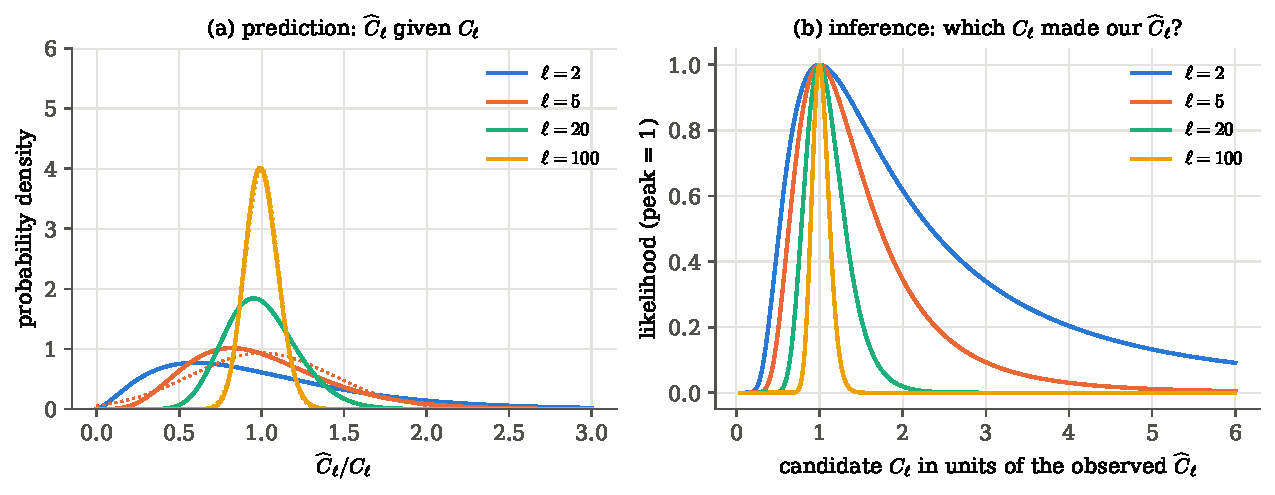
\includegraphics[width=0.98\linewidth]{figures/ch07/chat_pdf.pdf}
\caption{The two directions of the same formula. (a) Prediction: the density of $\Chat/\Cell$
for $\ell=2,5,20,100$, a scaled $\chi^2_{2\ell+1}$; dotted curves are Gaussians with the same mean
and variance, for $\ell=5$ and $\ell=100$. At low $\ell$ the estimator is skewed, with its mode
below the truth. (b) Inference: the likelihood of the true $\Cell$ given an observed $\Chat$,
normalised to peak $1$. All curves peak at the observed value; at low $\ell$ the likelihood has a
long tail towards large $\Cell$.}
\label{7b:fig:chat-pdf}
\end{figure}
\section{Where $\Cell$ and the skies come from: CAMB and HEALPix}
\label{7b:sec:camb-healpix}

Up to now $\Cell$ has been a given function and a sky has been a given set of $\alm$. In a real
analysis both have to be produced. The spectrum comes from physics: six cosmological numbers go
into a Boltzmann code, and $\Cell$ comes out (\cref{ch:T1}). The skies come from geometry: we
cut the sphere into pixels and use fast spherical-harmonic transforms to turn coefficients into
maps and maps back into coefficients. Think of the chain physical model $\to$ field or
dataset $\to$ summary $\to$ sampling distribution $\to$ inference. CAMB supplies the first arrow.
HEALPix lets us make the second arrow on a computer, as many times as we like.

\subsection{What CAMB computes}
\label{7b:sec:camb}

\emph{The input.} Follow one Fourier mode $\bm k$ of the primordial curvature perturbation
$\zeta$, the seed set up by inflation. Through gravity it perturbs
every component of the Universe: photons, baryons, cold dark matter, neutrinos and the metric.

\emph{What is followed.} The photon temperature perturbation in that mode depends on the
direction in which the photon travels, measured relative to $\bm k$. It is therefore expanded in
Legendre multipoles $\Theta_\ell(k,\eta)$, with $\eta$ the conformal time. The equations for these
multipoles form the \newterm{Boltzmann hierarchy}. For free-streaming particles it reads
\begin{equation}
  \Theta_\ell'=\frac{k}{2\ell+1}\bigl[\ell\,\Theta_{\ell-1}-(\ell+1)\,\Theta_{\ell+1}\bigr]
  \qquad(\ell\ge2),
  \label{7b:eq:hierarchy}
\end{equation}
where the prime is $\partial/\partial\eta$. In words: streaming moves anisotropy from each
multipole into its neighbours, and so from large angles to small. Photons obey the same equation
plus two extra terms: a Thomson scattering term, which damps every $\ell\ge2$ multipole while the
plasma is ionised, and gravitational source terms at $\ell\le2$.

\emph{What the code does.} A Boltzmann code integrates these coupled linear ODEs, together with
the fluid equations for baryons and dark matter and the linearised Einstein equations, from deep
in the radiation era to today, for a few thousand values of $k$. Integrating the hierarchy
directly up to $\ell\sim3000$ would be slow. The trick that made the codes fast is to write
today's multipoles as an integral along the line of sight,
$\Theta_\ell(k,\eta_0)=\int_0^{\eta_0}\dd\eta\,S(k,\eta)\,j_\ell\bigl(k(\eta_0-\eta)\bigr)$,
where the source $S$ needs only the first few multipoles and the spherical Bessel function
$j_\ell$ is pure geometry, independent of the cosmology \cite{Seljak1996}. CAMB implements this
method \cite{CAMB2000}; so do CMBFAST and CLASS, and all of them compute the linear CMB spectra
by integrating the sources along the photon line of sight \srcref{Padilla}{\S7.1.1}.

For statistics, what matters is the structure of the answer, and it is simple. The equations are
linear, so each $\bm k$ mode evolves on its own, and today's temperature in that mode is a fixed
number times its primordial amplitude $\zeta_{\bm k}$. That number, for multipole $\ell$, is the radiation
\newterm{transfer function} $g_{T\ell}(k)$ \unpack{the temperature anisotropy at multipole $\ell$
produced by one unit of $\zeta$ at wavenumber $k$, computed once per cosmology}. Projected on the
sky \cite{Seljak1996},
\begin{equation}
  \alm=4\pi\,i^\ell\int\frac{\dd^3k}{(2\pi)^3}\;g_{T\ell}(k)\,Y^*_{\ell m}(\hat{\bm k})\,\zeta_{\bm k} .
  \label{7b:eq:alm-transfer}
\end{equation}
With isotropic primordial statistics,
$\langle\zeta_{\bm k}\zeta^*_{\bm k'}\rangle=(2\pi)^3\delta^{(3)}(\bm k-\bm k')P_\zeta(k)$, the covariance
of the coefficients is
\begin{align}
  \langle\alm a^*_{\ell'm'}\rangle
  &\eqby{1}(4\pi)^2\,i^{\ell-\ell'}\!\int\!\frac{\dd^3k}{(2\pi)^3}\,g_{T\ell}(k)\,g_{T\ell'}(k)\,
     P_\zeta(k)\,Y^*_{\ell m}(\hat{\bm k})\,Y_{\ell'm'}(\hat{\bm k})
   \nonumber\\
  &\eqby{2}\frac{16\pi^2}{8\pi^3}\int_0^\infty k^2\dd k\;g_{T\ell}\,g_{T\ell'}\,P_\zeta(k)
     \int\dd\Omega_{\hat{\bm k}}\;Y^*_{\ell m}Y_{\ell'm'}
   \nonumber\\
  &\eqby{3}\underbrace{\frac{2}{\pi}\int_0^\infty k^2\dd k\;P_\zeta(k)\,g_{T\ell}(k)^2}_{\Cell}
     \;\delta_{\ell\ell'}\delta_{mm'} .
   \label{7b:eq:cl-transfer}
\end{align}
\begin{explain}
  \item Multiply \eqref{7b:eq:alm-transfer} by the conjugate of its primed copy, average, and do
        the $\bm k'$ integral with the delta function; $(i^{\ell'})^*=i^{-\ell'}$.
  \item Split $\dd^3k=k^2\dd k\,\dd\Omega_{\hat{\bm k}}$: the transfer functions and $P_\zeta$
        depend only on $k=|\bm k|$, the harmonics only on the direction $\hat{\bm k}$.
  \item Orthonormality \eqref{7b:eq:orthonormal} over the directions of $\bm k$ sets $\ell=\ell'$,
        $m=m'$, which also makes $i^{\ell-\ell'}=1$.
\end{explain}
This is the formula for $\Cell$ in \cref{ch:T1}. It is also the isotropy result
\eqref{7b:eq:alm-cov}, reached this time from the physics side. The Kronecker deltas came from
integrating the harmonics over the directions of $\bm k$, which was possible only because
$P_\zeta$ depends on $k=|\bm k|$ and not on the direction: that is where isotropy enters. The
formula carries three lessons. First, $\alm$ is a linear combination of Gaussian $\zeta_{\bm k}$, hence
Gaussian. Second, the whole cosmology sits in $P_\zeta$ (the amplitude $A_s$ and tilt $n_s$)
and in $g_{T\ell}$ (the other four parameters). Third, CAMB returns $\Cell$, an expectation value.
It never returns a sky; to get one we must draw the $\alm$ ourselves.

\paragraph{How to call it.} The fiducial spectra are computed once, in
\pyname{code/camb_fiducial.py}:
\pyfile[firstline=13,lastline=22,firstnumber=13]{code/camb_fiducial.py}{The CAMB call behind every fiducial spectrum}
\noindent Line 13 is the Planck 2018 best fit \cite{Planck2018VI} in CAMB's keywords (the
dictionary of \cref{ch:T1}). Line 18 builds a parameter object; computing to
$\ell_{\max}+200$ and setting \pyname{lens_potential_accuracy=1} keep the lensed spectra accurate up
to $\ell_{\max}=3000$. Line 19 solves the Boltzmann equations. Line 20 asks for the
\emph{raw} $\Cell$ in $\mu$K$^2$ (without \pyname{raw_cl=True} CAMB returns $D_\ell$, a factor
$\ell(\ell+1)/2\pi$ larger). Line 21 keeps the lensed total, with columns TT, EE, BB, TE. The
result is cached in \pyname{data/camb_fiducial.npz}, and every script loads it with
\pyname{load_fiducial()}, which returns $\ell$ and $C_\ell^{TT}$ with $C_0=C_1=0$. Rerunning CAMB
takes seconds, and is needed only when a script varies the parameters.

\paragraph{Example: the spectrum and its irreducible error bar.} \Cref{7b:fig:dl-band} shows the
fiducial $D_\ell=\ell(\ell+1)\Cell/2\pi$ with the band $D_\ell[1\pm\sqrt{2/(2\ell+1)}]$ of
\eqref{7b:eq:cv-frac}, and the $\widehat D_\ell$ of one simulated sky
(\pyname{code/ch07/24_camb_healpix.py}). The first acoustic peak is at $\ell=\SBpeakEll$ with
$D_\ell=\SBpeakD\,\mu$K$^2$; there the band is $\pm\sqrt{2/441}=\pm6.7\%$. At $\ell=2$ the band
is $\pm63\%$ wide and the one sky wanders through it; above $\ell\sim500$ the band is too thin to see
and the simulated points trace the curve. Large scales are known poorly from one sky, and nothing
can be done about it.

\begin{figure}[htbp]
\centering
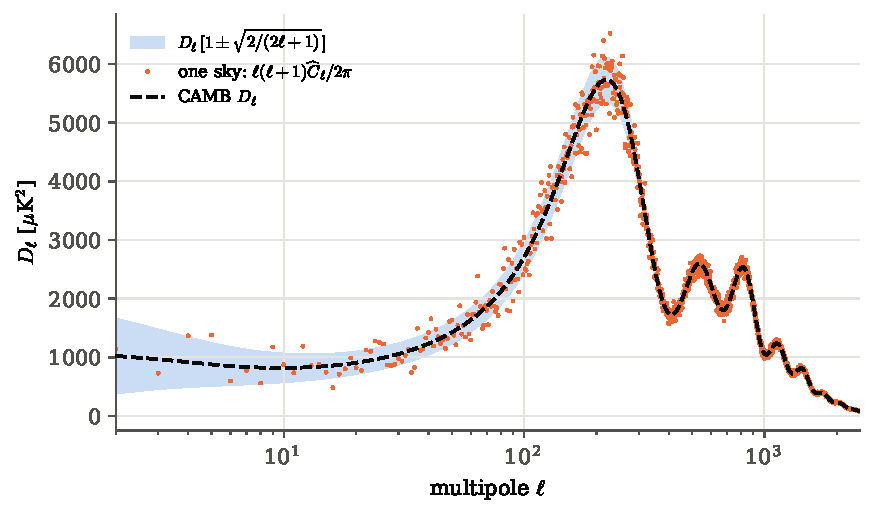
\includegraphics[width=0.72\linewidth]{figures/ch07/dl_band.pdf}
\caption{The fiducial CAMB spectrum $D_\ell$ (black dashed), its cosmic-variance band
$\pm\sqrt{2/(2\ell+1)}$ (blue), and the estimate $\ell(\ell+1)\Chat/2\pi$ from one simulated full
sky up to $\ell=\SBlmaxBand$ (orange points). The logarithmic $\ell$ axis stretches the few
low multipoles, where the band is wide, over a large part of the plot.}
\label{7b:fig:dl-band}
\end{figure}

\subsection{HEALPix: cutting the sphere into equal pixels}
\label{7b:sec:healpix}

A computer stores a map as a list of numbers, one per pixel, so we must cut the sphere into
pixels. Latitude--longitude grids are a poor choice. Their pixels shrink towards the poles. Noise
averaged over a small polar pixel then has a different variance from noise averaged over a
large equatorial one, so the map's noise changes with latitude. G\'orski et al.\ list
three properties a good pixelisation needs \cite{Gorski2005}:
\begin{enumerate}[itemsep=1pt]
  \item \emph{Equal areas}, so that white noise in time stays white noise in the map and every
        pixel samples the sky with the same weight;
  \item \emph{Pixel centres on rings of constant latitude}, so that spherical-harmonic transforms
        are fast: $Y_{\ell m}\propto P_\ell^m(\cos\theta)e^{im\phi}$, the expensive Legendre
        functions need to be evaluated once per ring rather than once per pixel, and the
        $e^{im\phi}$ sum along each ring is an FFT;
  \item \emph{A hierarchy}: each pixel splits into four at the next resolution, so that nearby
        pixels are nearby in memory.
\end{enumerate}

\begin{workdef}[HEALPix grid]
The \newterm{HEALPix} grid starts from $12$ equal-area base pixels and divides each into
$N_{\rm side}\times N_{\rm side}$ sub-pixels \unpack{$N_{\rm side}$ is a power of $2$ that sets
the resolution}. It has
\begin{equation}
  N_{\rm pix}=12\,N_{\rm side}^2\ \text{pixels},\qquad
  \Omega_{\rm pix}=\frac{4\pi}{N_{\rm pix}}=\frac{\pi}{3N_{\rm side}^2},\qquad
  4N_{\rm side}-1\ \text{rings of constant latitude},
  \label{7b:eq:healpix}
\end{equation}
and a full spherical-harmonic transform costs of order $N_{\rm pix}^{3/2}$ operations instead of
$N_{\rm pix}^2$ \cite{Gorski2005}, \srcref{Hivon}{p.~4}.
\end{workdef}

\Cref{7b:fig:healpix-tiling} shows the first three levels. The pixels are not squares (they are
curvilinear quadrilaterals, and near the poles they are visibly distorted), but they all have
exactly the same area.

\begin{figure}[htbp]
\centering
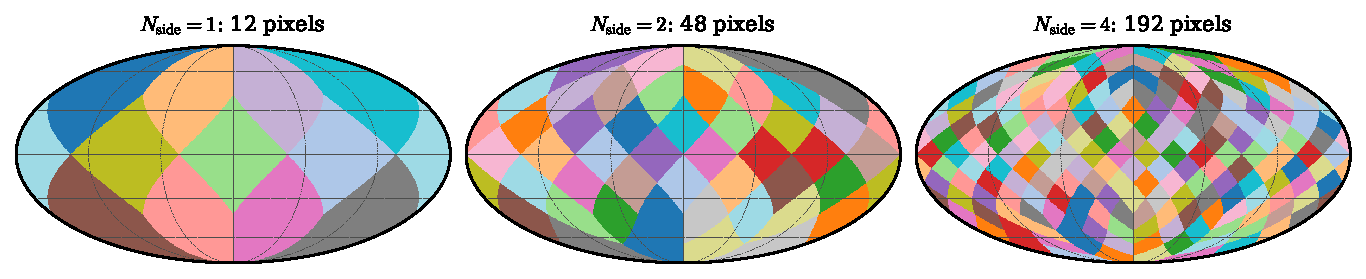
\includegraphics[width=0.98\linewidth]{figures/ch07/healpix_tiling.pdf}
\caption{HEALPix tilings with $N_{\rm side}=1$, $2$, $4$, each pixel painted a random colour,
with lines of latitude and longitude every $30^\circ$ and $60^\circ$. The twelve base pixels
form three rings of four; each step in $N_{\rm side}$ splits every pixel into four of equal
area.}
\label{7b:fig:healpix-tiling}
\end{figure}

\paragraph{Where the pixel edges come from.} The edges in \cref{7b:fig:healpix-tiling} look like
arbitrary curves, but every one of them follows from the demand for equal areas and an observation
of Archimedes. Wrap the unit sphere in a cylinder that touches it along the equator, and push each
point of the sphere straight out, away from the axis and at constant height, onto the cylinder
(\cref{7b:fig:healpix-cylinder}a). The point at polar angle $\theta$ and longitude $\phi$ lands at
the same $\phi$ and at height $z=\cos\theta$. This map keeps areas. Take the small patch between
$\theta$ and $\theta+\Delta\theta$ and between $\phi$ and $\phi+\Delta\phi$:
\begin{equation}
  \Delta\Omega\eqby{1}(\sin\theta\,\Delta\phi)\,(\Delta\theta)\eqby{2}\Delta\phi\,\abs{\Delta z} .
  \label{7b:eq:archimedes}
\end{equation}
\begin{explain}
  \item The patch is nearly a rectangle. Its width runs along the circle of latitude, whose radius
        is $\sin\theta$, so the width is $\sin\theta\,\Delta\phi$; its height runs along the meridian
        and is $\Delta\theta$.
  \item On the cylinder, of radius $1$, the same patch has width $\Delta\phi$ and height
        $\abs{\Delta z}$, and $z=\cos\theta$ gives $\abs{\Delta z}=\sin\theta\,\Delta\theta$.
\end{explain}

\begin{figure}[htbp]
\centering
\begin{tikzpicture}[font=\small,>=Stealth,scale=1.12,every node/.style={transform shape}]
  \begin{scope}
    \begin{scope}\clip (0,0) circle (1.7); \shade[inner color=white,outer color=black!25] (-0.5,0.6) circle (3.0);\end{scope}
    \draw[black!45] (0,0) circle (1.7);
    \draw[black!30,densely dotted,domain=180:360,samples=40,variable=\t] plot ({1.7*cos(\t)},{-0.9751*sin(\t)});
    \draw[black!30,domain=0:180,samples=40,variable=\t] plot ({1.7*cos(\t)},{-0.9751*sin(\t)});
    \draw[accent!70,domain=0:360,samples=60,variable=\t] plot ({1.7*cos(\t)},{1.3926-0.9751*sin(\t)});
    \draw[accent!70,domain=0:180,samples=40,variable=\t] plot ({1.7*cos(\t)},{-1.3926-0.9751*sin(\t)});
    \draw[accent!70,densely dotted,domain=180:360,samples=40,variable=\t] plot ({1.7*cos(\t)},{-1.3926-0.9751*sin(\t)});
    \draw[accent!70] (-1.7,-1.3926) -- (-1.7,1.3926) (1.7,-1.3926) -- (1.7,1.3926);
    \draw[->,black!55] (0,-1.3926) -- (0,2.45) node[above,font=\footnotesize] {$z$};
    \fill[fibreorange!85,draw=fibreorange!60!black,line width=0.6pt] plot[domain=0:1,samples=12,variable=\s] ({1.7*sqrt(1-(0.33333+\s*(0.33333))^2)*cos(67.5+\s*(22.5))},{1.3926*(0.33333+\s*(0.33333))-0.9751*sqrt(1-(0.33333+\s*(0.33333))^2)*sin(67.5+\s*(22.5))}) -- plot[domain=0:1,samples=12,variable=\s] ({1.7*sqrt(1-(0.66667+\s*(-0.33333))^2)*cos(90+\s*(22.5))},{1.3926*(0.66667+\s*(-0.33333))-0.9751*sqrt(1-(0.66667+\s*(-0.33333))^2)*sin(90+\s*(22.5))}) -- plot[domain=0:1,samples=12,variable=\s] ({1.7*sqrt(1-(0.33333+\s*(-0.33333))^2)*cos(112.5+\s*(-22.5))},{1.3926*(0.33333+\s*(-0.33333))-0.9751*sqrt(1-(0.33333+\s*(-0.33333))^2)*sin(112.5+\s*(-22.5))}) -- plot[domain=0:1,samples=12,variable=\s] ({1.7*sqrt(1-(0.00000+\s*(0.33333))^2)*cos(90+\s*(-22.5))},{1.3926*(0.00000+\s*(0.33333))-0.9751*sqrt(1-(0.00000+\s*(0.33333))^2)*sin(90+\s*(-22.5))}) -- cycle;
    \fill[fibreorange!60,fill opacity=0.35] plot[domain=0:1,samples=12,variable=\s] ({1.7*cos(67.5+\s*(22.5))},{1.3926*(0.33333+\s*(0.33333))-0.9751*sin(67.5+\s*(22.5))}) -- plot[domain=0:1,samples=12,variable=\s] ({1.7*cos(90+\s*(22.5))},{1.3926*(0.66667+\s*(-0.33333))-0.9751*sin(90+\s*(22.5))}) -- plot[domain=0:1,samples=12,variable=\s] ({1.7*cos(112.5+\s*(-22.5))},{1.3926*(0.33333+\s*(-0.33333))-0.9751*sin(112.5+\s*(-22.5))}) -- plot[domain=0:1,samples=12,variable=\s] ({1.7*cos(90+\s*(-22.5))},{1.3926*(0.00000+\s*(0.33333))-0.9751*sin(90+\s*(-22.5))}) -- cycle;
    \draw[fibreorange!55!black,line width=0.9pt] plot[domain=0:1,samples=12,variable=\s] ({1.7*cos(67.5+\s*(22.5))},{1.3926*(0.33333+\s*(0.33333))-0.9751*sin(67.5+\s*(22.5))}) -- plot[domain=0:1,samples=12,variable=\s] ({1.7*cos(90+\s*(22.5))},{1.3926*(0.66667+\s*(-0.33333))-0.9751*sin(90+\s*(22.5))}) -- plot[domain=0:1,samples=12,variable=\s] ({1.7*cos(112.5+\s*(-22.5))},{1.3926*(0.33333+\s*(-0.33333))-0.9751*sin(112.5+\s*(-22.5))}) -- plot[domain=0:1,samples=12,variable=\s] ({1.7*cos(90+\s*(-22.5))},{1.3926*(0.00000+\s*(0.33333))-0.9751*sin(90+\s*(-22.5))}) -- cycle;
    \foreach \p/\z in {67.5/0.33333,90/0.66667,112.5/0.33333}
      \draw[->,black,densely dashed,line width=0.5pt,shorten >=0.5pt] ({1.7*sqrt(1-(\z)^2)*cos(\p)},{1.3926*(\z)-0.9751*sqrt(1-(\z)^2)*sin(\p)}) -- ({1.7*cos(\p)},{1.3926*(\z)-0.9751*sin(\p)});
    \draw[black!70,dashed,line width=0.5pt,domain=15:140,samples=40,variable=\t] plot ({1.7*cos(\t)},{1.3926*(0.33333)-0.9751*sin(\t)});
    \draw[black!70,dashed,line width=0.5pt,domain=15:140,samples=40,variable=\t] plot ({1.7*cos(\t)},{1.3926*(0.66667)-0.9751*sin(\t)});
    \draw[<->,black,line width=0.6pt] ({1.7*cos(22)},{1.3926*(0.33333)-0.9751*sin(22)}) -- ({1.7*cos(22)},{1.3926*(0.66667)-0.9751*sin(22)}) node[midway,right,font=\footnotesize] {$\Delta z$};
    \draw[black!70,dashed,line width=0.5pt] ({1.7*cos(67.5)},{1.3926*(0.33333)-0.9751*sin(67.5)}) -- ({1.7*cos(67.5)},{1.3926*(-0.22)-0.9751*sin(67.5)}) ({1.7*cos(112.5)},{1.3926*(0.33333)-0.9751*sin(112.5)}) -- ({1.7*cos(112.5)},{1.3926*(-0.22)-0.9751*sin(112.5)});
    \draw[<->,black,line width=0.6pt,domain=68.5:111.5,samples=16,variable=\t] plot ({1.7*cos(\t)},{1.3926*(-0.16)-0.9751*sin(\t)});
    \node[font=\footnotesize,anchor=north] at ({1.7*cos(90)},{1.3926*(-0.2)-0.9751*sin(90)}) {$\Delta\phi$};
    \node[font=\scriptsize,fibreorange!90!black,align=center] at (-1.05,1.35) {pixel on\\[-2pt]the sphere};
    \draw[fibreorange!90!black,->,shorten >=1pt] (-0.75,1.15) .. controls (-0.3,1.0) .. ({1.7*sqrt(1-(0.55)^2)*cos(90)},{1.3926*(0.55)-0.9751*sqrt(1-(0.55)^2)*sin(90)});
    \node[font=\scriptsize,fibreorange!70!black,align=left,anchor=west] at (1.85,1.75) {its image on\\[-2pt]the cylinder};
    \draw[fibreorange!70!black,->,shorten >=1pt] (1.95,1.5) -- ({1.7*cos(76)},{1.3926*(0.45)-0.9751*sin(76)});
    \node[font=\small] at (0,-2.85) {(a)};
  \end{scope}
  \begin{scope}[shift={(4.75,0)},x=0.95cm,y=2.0cm]
    \draw[black!40] (0,-1) rectangle ({2*pi},1);
    \draw[black!35,densely dashed] (0,{2/3}) -- ({2*pi},{2/3}) (0,{-2/3}) -- ({2*pi},{-2/3});
    \begin{scope}
      \clip (0,{-2/3}) rectangle ({2*pi},{2/3});
      \foreach \k in {0,...,10} {
        \pgfmathsetmacro\w{mod(\k,2)==0 ? 1.1 : 0.45}
        \draw[accent,line width=\w pt] (0,{2/3-2*\k/3}) -- ({2*pi},{2/3-2*\k/3+16/3});
        \draw[accent,line width=\w pt] (0,{-2/3+2*\k/3}) -- ({2*pi},{-2/3+2*\k/3-16/3});
      }
    \end{scope}
    \foreach \q in {0,1,2,3} {
      \pgfmathsetmacro\a{\q*pi/2}
      \foreach \s in {1,-1} {
        \draw[accent,line width=1.1pt] (\a,{\s*2/3}) -- (\a,\s);
        \foreach \k in {1} {
          \pgfmathsetmacro\lo{\k*pi/4}\pgfmathsetmacro\hi{pi/2-\k*pi/4}
          \draw[accent,line width=0.45pt,domain=\lo:1.5708,samples=30,variable=\t]
            plot ({\a+\t},{\s*(1-(\k*\k/12)*(pi/(2*\t))^2)});
          \draw[accent,line width=0.45pt,domain=0:\hi,samples=30,variable=\t]
            plot ({\a+\t},{\s*(1-(\k*\k/12)*(pi/(pi-2*\t))^2)});
        }
      }
    }
    
    \foreach \x/\l in {0/0,{pi/2}/{\pi/2},{pi}/{\pi},{3*pi/2}/{3\pi/2},{2*pi}/{2\pi}}
      \node[font=\scriptsize,below] at (\x,-1) {$\l$};
    \node[font=\footnotesize] at ({pi},-1.27) {$\phi$};
    \foreach \y/\l in {-1/{-1},{-2/3}/{-\frac23},0/0,{2/3}/{\frac23},1/1}
      \node[font=\scriptsize,left] at (0,\y) {$\l$};
    \node[font=\footnotesize] at (-0.7,0) {$z$};
    \def\pc{1.5708}\def\dph{0.7854}
    \fill[fibreorange!85,draw=fibreorange!60!black,line width=0.8pt] ({\pc-\dph/2},{1/3}) -- (\pc,{2/3}) -- ({\pc+\dph/2},{1/3}) -- (\pc,0) -- cycle;
    \draw[black!75,dashed,line width=0.5pt] ({\pc-0.45},{1/3}) -- ({\pc+1.25},{1/3}) ({\pc-0.45},{2/3}) -- ({\pc+1.25},{2/3});
    \draw[<->,black,line width=0.6pt] ({\pc+0.75},{1/3}) -- ({\pc+0.75},{2/3});
    \node[font=\scriptsize,anchor=west,fill=white,inner sep=1pt] at ({\pc+0.8},0.5) {$\Delta z$};
    \draw[black!75,dashed,line width=0.5pt] ({\pc-\dph/2},{1/3}) -- ({\pc-\dph/2},-0.22) ({\pc+\dph/2},{1/3}) -- ({\pc+\dph/2},-0.22);
    \draw[<->,black,line width=0.6pt] ({\pc-\dph/2},-0.16) -- ({\pc+\dph/2},-0.16);
    \node[font=\scriptsize,anchor=north,fill=white,inner sep=1pt] at (\pc,-0.2) {$\Delta\phi$};
    \node[font=\scriptsize,anchor=west,fill=white,inner sep=1pt] at ({\pc+1.27},{1/3}) {$z_j$};
    \node[font=\scriptsize,anchor=west,fill=white,inner sep=1pt] at ({\pc+1.27},{2/3}) {$z_{j+1}$};
    \node[font=\scriptsize,softgray,anchor=west] at ({2*pi+0.1},0.83) {polar cap};
    \node[font=\scriptsize,softgray,anchor=west] at ({2*pi+0.1},0) {equatorial};
    \node[font=\scriptsize,softgray,anchor=west] at ({2*pi+0.1},-0.12) {belt};
    \node[font=\scriptsize,softgray,anchor=west] at ({2*pi+0.1},-0.83) {polar cap};
    \node[font=\small] at ({pi},-1.48) {(b)};
  \end{scope}
\end{tikzpicture}
\caption{Archimedes' map and the HEALPix edges. (a) Each point of the sphere is pushed straight out,
at constant height, onto the cylinder that touches the sphere along the equator. One pixel for
$N_{\rm side}=2$ is shown on the sphere (solid) and as its image on the cylinder (see-through); the
dashed rings $z_j$ and $z_{j+1}$ and the dashed lines below its side corners mark $\Delta z$ and
$\Delta\phi$ on the cylinder. (b) The cylinder cut open along $\phi=0$ and laid flat. The thick
lines are the boundaries of the twelve base pixels, the thin ones those for $N_{\rm side}=2$:
straight \eqref{7b:eq:hpx-belt} in the belt $\abs z\le\tfrac23$, curved \eqref{7b:eq:hpx-cap} in the
two polar caps. The same pixel is shaded: its width along its ring is $\Delta\phi=\pi/(2N_{\rm side})$,
and the rings $z_j$ and $z_{j+1}$ of pixel centres are $\Delta z=2/(3N_{\rm side})$ apart
\eqref{7b:eq:hpx-dphidz}, so its area is $\Delta\phi\,\Delta z=\Omega_{\rm pix}$.}
\label{7b:fig:healpix-cylinder}
\end{figure}

The image on the cylinder is wider than the patch by $1/\sin\theta$ and shorter by $\sin\theta$,
and the two factors cancel. Now cut the cylinder open along $\phi=0$ and lay it flat: a rectangle
$0\le\phi<2\pi$, $-1\le z\le1$, of area $4\pi$ (\cref{7b:fig:healpix-cylinder}b). A region of the
sphere has the same area as its image in this rectangle, so \emph{equal-area pixels on the sphere
are the same thing as equal-area tiles in the flat $(\phi,z)$ rectangle}. We design the tiles
there.

\emph{The equatorial belt.} Here the pixels are laid out in rings of constant $z$, and every ring
holds the same number of pixels, $4N_{\rm side}$: the equator crosses four base pixels, each
$N_{\rm side}$ pixels across. Two numbers then fix everything, the width $\Delta\phi$ of a pixel
along its ring and the spacing $\Delta z$ between neighbouring rings (\cref{7b:fig:healpix-cylinder}b):
\begin{equation}
  \Delta\phi\eqby{1}\frac{2\pi}{4N_{\rm side}}=\frac{\pi}{2N_{\rm side}},
  \qquad
  \Delta z\eqby{2}\frac{\Omega_{\rm pix}}{\Delta\phi}
  \eqby{3}\frac{\pi/(3N_{\rm side}^2)}{\pi/(2N_{\rm side})}=\frac{2}{3N_{\rm side}} .
  \label{7b:eq:hpx-dphidz}
\end{equation}
\begin{explain}
  \item A ring goes once round, $2\pi$, and holds $4N_{\rm side}$ pixels.
  \item In the flat picture area is $\Delta\phi\,\Delta z$, and each pixel must have area
        $\Omega_{\rm pix}$.
  \item $\Omega_{\rm pix}=\pi/(3N_{\rm side}^2)$ from \eqref{7b:eq:healpix}.
\end{explain}
The rings of pixel centres in the belt are therefore at
\begin{equation}
  z_j=j\,\Delta z=\frac{2j}{3N_{\rm side}},\qquad
  \cos\theta_j=\frac{2j}{3N_{\rm side}},\qquad j=-N_{\rm side},\dots,N_{\rm side},
  \label{7b:eq:hpx-rings}
\end{equation}
and the belt ends at $j=\pm N_{\rm side}$, $z=\pm\tfrac23$, which is where the number $\tfrac23$ in
HEALPix comes from. If the pixels of neighbouring rings sat directly above one another, they would
be rectangles $\Delta\phi\times\Delta z$. HEALPix instead shifts each ring by half a pixel,
$\Delta\phi/2$, against its neighbours, so a pixel centre sits directly above the gap between two
pixels of the ring below. The pixel around the centre $(\phi_c,z_j)$ is then the diamond with
corners at $(\phi_c\pm\tfrac12\Delta\phi,\,z_j)$ on its own ring and at $(\phi_c,\,z_j\pm\Delta z)$,
the centres' height of the rings above and below. Its area is half the product of its diagonals,
$\tfrac12\,\Delta\phi\cdot2\Delta z=\Delta\phi\,\Delta z=\Omega_{\rm pix}$, as required, and its
edges are straight lines of slope
\begin{equation}
  \pm\frac{\Delta z}{\Delta\phi/2}=\pm\frac{2/(3N_{\rm side})}{\pi/(4N_{\rm side})}=\pm\frac{8}{3\pi},
\end{equation}
the same for every $N_{\rm side}$. Edges of the same slope pass through corners that are $\Delta\phi$
apart along a ring, so their values at $\phi=0$ differ by
$\tfrac{8}{3\pi}\Delta\phi=\tfrac{4}{3N_{\rm side}}$, and one of them passes through the corner at
$(0,\tfrac23)$. The pixel edges in the belt are thus
\begin{equation}
  z=\frac23-\frac{4k}{3N_{\rm side}}\pm\frac{8\phi}{3\pi},
  \qquad k\ \text{an integer},\quad\abs z\le\frac23 ,
  \label{7b:eq:hpx-belt}
\end{equation}
straight lines on the flat rectangle and curves with $\cos\theta$ linear in $\phi$ on the sphere.
For $N_{\rm side}=1$ the same construction gives the twelve base pixels: four diamonds
$\Delta\phi=\tfrac\pi2$ wide and $2\Delta z=\tfrac43$ tall around the equator, with the four northern
and four southern base pixels filling the triangles between them.

\emph{The polar caps.} Above $z=\tfrac23$ the flat picture has a strip of height $\tfrac13$ and
area $2\pi/3$. It belongs to the four northern base pixels. The lower part of each, a triangle
between two equatorial diamonds, has area $\tfrac12\cdot\tfrac\pi2\cdot\tfrac23=\tfrac\pi6$, so the
remaining $\tfrac\pi6$ of each is a quarter of the strip, a rectangle
$\phi_t\in[0,\tfrac\pi2]$, $z\in[\tfrac23,1]$, where $\phi_t$ is $\phi$ measured from the start of
its quarter. Diamonds cannot tile it, because its top edge $z=1$ is not a line on the sphere but a
single point, the pole: on the sphere the rectangle is a triangle with one corner at the pole. We
need coordinates in which it is drawn as a triangle and areas are still uniform. Near the pole
$1-z=1-\cos\theta\approx\theta^2/2$, so $\sqrt{1-z}$ measures distance from the pole. Set
\begin{equation}
  \rho=\sqrt{3(1-z)},\qquad
  u=\frac{2\phi_t}{\pi}\,\rho,\qquad
  v=\Bigl(1-\frac{2\phi_t}{\pi}\Bigr)\rho .
  \label{7b:eq:hpx-uv}
\end{equation}
The pole, $\rho=0$, becomes the single point $u=v=0$. The edge $\phi_t=0$ becomes $u=0$, the edge
$\phi_t=\tfrac\pi2$ becomes $v=0$, and the bottom edge $z=\tfrac23$, where $\rho=1$, becomes the line
$u+v=1$. The quarter-cap is the triangle $u,v\ge0$, $u+v\le1$, half of a unit square. Its areas are
uniform:
\begin{equation}
  \Delta\Omega\eqby{1}\abs{\Delta z}\,\Delta\phi_t
  \eqby{2}\frac{2\rho}{3}\,\Delta\rho\,\Delta\phi_t
  \eqby{3}\frac{\pi}{3}\,\Delta u\,\Delta v .
  \label{7b:eq:hpx-jac}
\end{equation}
\begin{explain}
  \item Archimedes' rule \eqref{7b:eq:archimedes}.
  \item $z=1-\rho^2/3$, so $\abs{\Delta z}=\tfrac{2\rho}{3}\Delta\rho$.
  \item The area of a small cell in the $(u,v)$ plane is the Jacobian times $\Delta\rho\,\Delta\phi_t$:
        with $\partial u/\partial\rho=2\phi_t/\pi$, $\partial u/\partial\phi_t=2\rho/\pi$,
        $\partial v/\partial\rho=1-2\phi_t/\pi$ and $\partial v/\partial\phi_t=-2\rho/\pi$, the
        determinant is $-\tfrac{2\phi_t}{\pi}\tfrac{2\rho}{\pi}-\tfrac{2\rho}{\pi}\bigl(1-\tfrac{2\phi_t}{\pi}\bigr)=-\tfrac{2\rho}{\pi}$,
        so $\Delta u\,\Delta v=\tfrac{2\rho}{\pi}\Delta\rho\,\Delta\phi_t$; replace
        $\tfrac{2\rho}{3}\Delta\rho\,\Delta\phi_t$ by $\tfrac{\pi}{3}\Delta u\,\Delta v$.
\end{explain}
The factor $\pi/3$ is the same everywhere, so equal areas in the $(u,v)$ triangle are equal areas on
the sphere (the whole triangle, of area $\tfrac12$, is $\tfrac\pi6$, as it should be). In the
triangle we can again cut with straight lines, $u=k/N_{\rm side}$ and $v=k/N_{\rm side}$, into
squares of area $1/N_{\rm side}^2$, each a pixel of area $\tfrac{\pi}{3N_{\rm side}^2}=\Omega_{\rm
pix}$; the squares cut in half by $u+v=1$ are completed by the half-diamonds just below
$z=\tfrac23$, since at $\rho=1$ the line $u=k/N_{\rm side}$ sits at $\phi_t=k\pi/(2N_{\rm side})$,
exactly where the belt edge \eqref{7b:eq:hpx-belt} with the same $k$ reaches $z=\tfrac23$. Turning
the straight lines back into $(\phi,z)$ with \eqref{7b:eq:hpx-uv}: $u=k/N_{\rm side}$ means
$\tfrac{2\phi_t}{\pi}\sqrt{3(1-z)}=\tfrac{k}{N_{\rm side}}$; square both sides and solve for $z$, and
do the same for $v$:
\begin{equation}
  z=1-\frac{k^2}{3N_{\rm side}^2}\Bigl(\frac{\pi}{2\phi_t}\Bigr)^2,
  \qquad
  z=1-\frac{k^2}{3N_{\rm side}^2}\Bigl(\frac{\pi}{\pi-2\phi_t}\Bigr)^2 ,
  \qquad z\ge\frac23 ,
  \label{7b:eq:hpx-cap}
\end{equation}
and the same with $z\to-z$ in the south. These are the curved edges near the top and bottom of
\cref{7b:fig:healpix-cylinder}b, and \eqref{7b:eq:hpx-belt} and \eqref{7b:eq:hpx-cap} are the pixel
boundaries of \cite{Gorski2005}. The corners again sit on rings: where $u=k/N_{\rm side}$ meets
$v=j/N_{\rm side}$, $\rho=u+v=(k+j)/N_{\rm side}$ and $z=1-(k+j)^2/(3N_{\rm side}^2)$.

\paragraph{Example: pixel sizes and band limits.} The side of a pixel is about the square root
of its area,
\begin{equation}
  \theta_{\rm pix}\approx\sqrt{\Omega_{\rm pix}}=\sqrt{\frac{\pi}{3}}\,\frac{1}{N_{\rm side}}\ \text{rad}
  =\frac{58.6^\circ}{N_{\rm side}} .
  \label{7b:eq:pixsize}
\end{equation}
For $N_{\rm side}=256$ that is $\SBpixTwoFiveSix'$ with $\SBnpixTwoFiveSix$ pixels; $N_{\rm
side}=512$ gives $\SBpixFiveTwelve'$ and $\SBnpixFiveTwelve$ pixels; Planck's high-frequency maps
use $N_{\rm side}=2048$, $\SBpixTwoK'$ and $\SBnpixTwoK$ pixels. How high in $\ell$ can a map of
$N_{\rm pix}$ numbers go? A sky band-limited to $\ell_{\max}$ has $(\ell_{\max}+1)^2$ real degrees of
freedom (\cref{7b:sec:alm}), and $N_{\rm pix}$ numbers cannot determine more than $N_{\rm pix}$
unknowns:
\begin{equation}
  (\ell_{\max}+1)^2\le12N_{\rm side}^2
  \quad\Longrightarrow\quad
  \ell_{\max}\lesssim\sqrt{12}\,N_{\rm side}\approx3.5\,N_{\rm side} .
  \label{7b:eq:bandlimit}
\end{equation}
In practice healpy never goes beyond $\ell_{\max}=3N_{\rm side}-1$, and analyses that need
accurate coefficients stay below about $2N_{\rm side}$, as the next example shows.

\subsection{healpy: four operations and their from-scratch versions}
\label{7b:sec:healpy}

The Python package healpy wraps the HEALPix library. Four functions do everything in this
chapter, and two more are shorthands (\cref{7b:fig:pipeline}):
\begin{itemize}[itemsep=1pt]
  \item \pyname{synalm(cl, lmax)}: draw one set of Gaussian $\alm$ with spectrum $\Cell$;
  \item \pyname{alm2map(alm, nside)}: sum the series \eqref{7b:eq:alm} at every pixel centre;
  \item \pyname{map2alm(map, lmax, iter)}: compute the coefficients of a map;
  \item \pyname{alm2cl(alm)}: the estimator $\Chat$ of \eqref{7b:eq:chat};
  \item \pyname{synfast} $=$ \pyname{synalm} then \pyname{alm2map}, and \pyname{anafast} $=$
        \pyname{map2alm} then \pyname{alm2cl}.
\end{itemize}

\begin{figure}[htbp]
\centering
\begin{tikzpicture}[font=\small,
  obj/.style={draw=accent,thick,rounded corners=2pt,fill=ideabg,minimum width=17mm,
              minimum height=8mm,align=center},
  fn/.style={draw=softgray,rounded corners=6pt,fill=black!4,minimum height=6mm,
             font=\ttfamily\footnotesize,align=center},
  flow/.style={->,thick,accent}]
  \node[obj] (cl) at (0,0) {$\Cell$\\[-1pt]{\scriptsize CAMB}};
  \node[fn]  (f1) at (2.3,0) {synalm};
  \node[obj] (a1) at (4.6,0) {$\alm$};
  \node[fn]  (f2) at (6.9,0) {alm2map};
  \node[obj] (mp) at (9.4,0) {map\\[-1pt]{\scriptsize $N_{\rm pix}$ values}};
  \node[fn]  (f3) at (9.4,-1.7) {map2alm};
  \node[obj] (a2) at (6.9,-1.7) {$\alm$};
  \node[fn]  (f4) at (4.6,-1.7) {alm2cl};
  \node[obj] (ch) at (2.3,-1.7) {$\Chat$};
  \draw[flow] (cl) -- (f1); \draw[flow] (f1) -- (a1); \draw[flow] (a1) -- (f2);
  \draw[flow] (f2) -- (mp); \draw[flow] (mp) -- (f3); \draw[flow] (f3) -- (a2);
  \draw[flow] (a2) -- (f4); \draw[flow] (f4) -- (ch);
  \draw[decorate,decoration={brace,amplitude=5pt}] (1.7,0.55) -- (7.5,0.55);
  \node[anchor=south] at (4.6,0.75) {\texttt{synfast}};
  \draw[decorate,decoration={brace,amplitude=5pt,mirror}] (4.0,-2.25) -- (10.0,-2.25);
  \node[anchor=north] at (7.0,-2.45) {\texttt{anafast}};
  \node[anchor=east,align=right,font=\scriptsize,softgray] at (1.3,-1.7)
    {compare with\\the input $\Cell$};
\end{tikzpicture}
\caption{The healpy pipeline. Objects are in blue boxes, functions in grey. \texttt{synfast}
draws coefficients from a spectrum and turns them into a map; \texttt{anafast} turns a map back
into coefficients and squares them into $\Chat$. Comparing the output $\Chat$ with the input
$\Cell$, over many skies, is the Monte Carlo study of \cref{7b:sec:mc}.}
\label{7b:fig:pipeline}
\end{figure}

\paragraph{Storage.} healpy stores only the coefficients with $m\ge0$, since the others follow
from the reality condition \eqref{7b:eq:reality}. They are ordered by $m$ first: all $\ell$ for
$m=0$, then all $\ell\ge1$ for $m=1$, and so on, so that $\alm$ sits at position
$m(2\ell_{\max}+1-m)/2+\ell$. For $\ell_{\max}=20$, the coefficient $a_{5,3}$ is at
$3\times38/2+5=62$, which is what \pyname{healpy.Alm.getidx(20, 5, 3)} returns. Neighbouring
$\ell$ at fixed $m$ are neighbours in memory, which is what made the modulation code of
\cref{7b:sec:iso-test} so short.

\paragraph{Drawing a sky by hand.} To see the mechanism we first write
\pyname{synalm} ourselves, straight from the table of real degrees of freedom in \cref{7b:sec:dof}:
\pyfile[firstline=34,lastline=45,firstnumber=34]{code/ch07/lib_harmonic.py}{Isotropic Gaussian coefficients from a spectrum}
\noindent Line 42 gives every stored coefficient the standard deviation $\sqrt{\Cell}$ of its
multipole. Lines 43--44 draw two standard normals per coefficient. Line 45 is the table: for
$m=0$ the coefficient is real with variance $\Cell$ (the imaginary draw is discarded); for $m>0$
the real and imaginary parts are each $\sqrt{\Cell/2}$ times a standard normal. Nothing else is
needed for an isotropic Gaussian sky, because the coefficients are independent: this is the
diagonal Cholesky factor of \cref{ch:06}, one $\sqrt{\Cell}$ per mode. The library function
\pyname{healpy.synalm} does the same with numpy's global random stream; in \cref{7b:sec:mc} we
check that the two produce statistically identical skies.

\paragraph{From a map back to coefficients.} The integral \eqref{7b:eq:alm} becomes a sum over
pixels, $\alm\approx\Omega_{\rm pix}\sum_p\Theta(p)\,Y^*_{\ell m}(p)$ \srcref{Hivon}{(12)}, with
$\Omega_{\rm pix}$ the pixel area of \eqref{7b:eq:healpix}. That sum is a quadrature rule, and it
is not exact. healpy improves it by iteration (\pyname{iter}): synthesise a map from the current
coefficients, analyse the difference between that map and the input map, and add the correction.

How accurate is the round trip $\alm\to$ map $\to\alm$? We test it at $N_{\rm side}=256$
(\cref{7b:fig:roundtrip}) with the script
\pyname{code/ch07/}\allowbreak\pyname{24_camb_healpix.py}. For a sky band-limited to $\ell\le2N_{\rm side}=512$, the recovered
$\Chat$ agrees with that of the input coefficients to a median relative error of $\SBrtZero$
without iteration, and $\SBrtThree$ with three iterations (the worst multipole is off by
$\SBrtThreeMax$). Now let the sky contain power up to $3N_{\rm side}-1=767$. The pixels can no
longer tell the highest multipoles apart from lower ones, so power leaks downwards
(\newterm{aliasing}). The error below $\ell=512$ rises to a median of $\SBrtAlias$, and near
$\ell=3N_{\rm side}$ it reaches ten percent.

\begin{figure}[htbp]
\centering
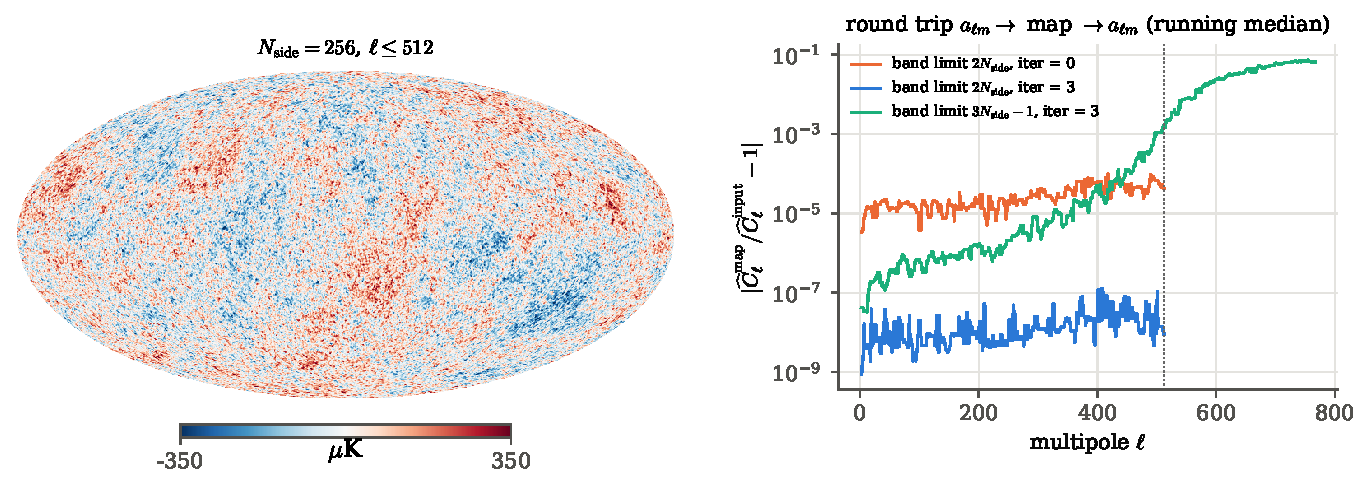
\includegraphics[width=0.98\linewidth]{figures/ch07/roundtrip.pdf}
\caption{Left: a simulated sky at $N_{\rm side}=256$ with $\ell\le512$. Right: relative difference
between $\Chat$ measured on the map (\texttt{anafast}) and $\Chat$ of the coefficients the map
was made from, smoothed with a running median over $9$ multipoles. Iterating the quadrature
(blue) gains three orders of magnitude over a single pass (orange). With power up to
$3N_{\rm side}-1$ (green), aliasing spoils the high multipoles. The dotted line marks
$\ell=2N_{\rm side}$.}
\label{7b:fig:roundtrip}
\end{figure}

\begin{pitfall}[A map is not a band-limited sky]
The real sky has power at every $\ell$, and a pixel averages the sky over its area. Both effects
change the measured spectrum: power above the band limit aliases into lower multipoles, and the
pixel average multiplies $\Cell$ by the square of a \emph{pixel window function} (healpy's
\pyname{pixwin}), just as a beam multiplies it by $B_\ell^2$ \srcref{Hivon}{(15)}. A simulation
that draws $\alm$ only up to $\ell_{\max}$ and analyses at the same $\ell_{\max}$ sees neither effect.
Choose $N_{\rm side}$ so that the beam has already killed the signal well below
$2N_{\rm side}$, and include the pixel window when comparing with data (\cref{ch:08}).
\end{pitfall}
\section{Cosmic variance by Monte Carlo}
\label{7b:sec:mc}

We now have two independent routes to the same numbers. Algebra gave the exact sampling
distribution of $\Chat$ (\cref{7b:sec:cosmic-variance}): a scaled $\chi^2_{2\ell+1}$ with variance
$2\Cell^2/(2\ell+1)$. The tools of \cref{7b:sec:camb-healpix} let us make as many skies as we like
from the CAMB spectrum. If we draw many skies, measure $\Chat$ on each, and histogram the results,
the histogram must reproduce the algebra. The comparison does two jobs. It checks every step of
the derivation: the reality condition, the counting, the factor of two. And it builds, where the
right answer is known, the same machine that \cref{ch:08} will use where no answer is known.

\paragraph{The questions.} With $N$ simulated full skies from the fiducial $\Cell$:
\begin{enumerate}[itemsep=1pt]
  \item Does the histogram of $\Chat$ at a given $\ell$ follow the scaled $\chi^2_{2\ell+1}$?
  \item Does the Monte Carlo variance of $\Chat$ converge to $2\Cell^2/(2\ell+1)$, and how fast:
        how large is the Monte Carlo error on a Monte Carlo variance?
  \item Is the covariance between different multipoles zero, and what does ``zero'' look like
        when it is estimated from $N$ skies?
\end{enumerate}

\subsection{The simulation}
\label{7b:sec:mc-sim}

The script \pyname{code/ch07/25_mc_cosmic_variance.py} simulates $N=\SBNsim$ full skies for
$2\le\ell\le300$. It does not build maps. On the full sky a map is a lossless re-encoding of
the coefficients: \cref{7b:fig:roundtrip} showed that the round trip returns them to a part in
$10^8$. So drawing the coefficients and applying \eqref{7b:eq:chat} is the same experiment,
thousands of times faster. For each multipole the script draws the $2\ell+1$ real numbers of the
table in \cref{7b:sec:dof} directly:
\pyfile[firstline=59,lastline=71,firstnumber=59]{code/ch07/lib_harmonic.py}{$\Chat$ for many independent skies, one multipole at a time}
\noindent Line 67 draws a block of standard normals, one row per sky and $2\ell+1$ columns.
Line 68 turns the first column into $a_{\ell0}$, with variance $\Cell$; line 69 turns the other
$2\ell$ columns into the real and imaginary parts of $a_{\ell1},\dots,a_{\ell\ell}$, each with
variance $\Cell/2$. Line 70 is the estimator \eqref{7b:eq:chat} with the factor $2$ for the
negative $m$. Nowhere does the code use the $\chi^2$ result; it only uses the covariance
\eqref{7b:eq:alm-cov} and the reality condition. The driver is short:
\pyfile[firstline=27,lastline=34,firstnumber=27]{code/ch07/25_mc_cosmic_variance.py}{The Monte Carlo run}
\noindent Line 32 returns an array with one row per sky and one column per multipole; line 33
divides by the input spectrum, so that every column of \pyname{y} should have mean $1$ and
variance $2/(2\ell+1)$. The run draws about $1.8\times10^9$ Gaussian numbers and takes
under a minute.

\subsection{The sampling distribution of $\Chat$}
\label{7b:sec:mc-dist}

The first question has a clear answer: yes. \Cref{7b:fig:mc-histograms} compares the histograms
of $\Chat/\Cell$ at $\ell=2$, $10$, $50$ and $300$ with the scaled $\chi^2_{2\ell+1}$ density
\eqref{7b:eq:chat-pdf}. The agreement is visible by eye, including the strong skew at $\ell=2$.
There the Gaussian of the same mean and variance (dotted) is plainly wrong: it puts probability
on negative power and misses the peak. For a quantitative check we use the Kolmogorov--Smirnov test of \cref{ch:04}, with the null hypothesis
``$(2\ell+1)\Chat/\Cell$ is $\chi^2_{2\ell+1}$''. The $p$-values are $\SBksTwo$, $\SBksTen$,
$\SBksFifty$ and $\SBksThree$: with $\SBNsim$ skies per multipole, nothing distinguishes the
simulation from the scaled $\chi^2$. The mean is right too: the average of $\Chat/\Cell$ over all
skies is $1$ at every one of the $299$ multipoles. The largest deviation, in units of its standard error
$\sqrt{2/[(2\ell+1)N]}$, is $\SBmeanDevMax$, which is the typical size of the largest of $299$
independent standard normal deviations. The estimator is unbiased.

\begin{figure}[htbp]
\centering
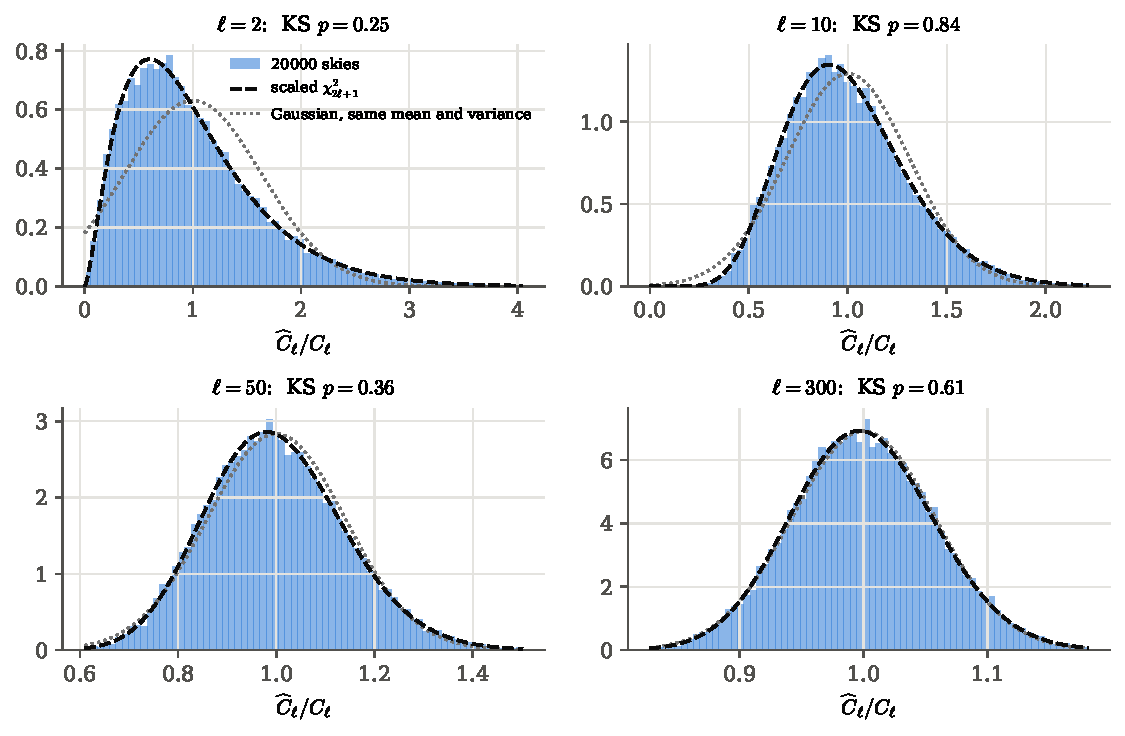
\includegraphics[width=0.85\linewidth]{figures/ch07/mc_histograms.pdf}
\caption{Histograms of $\Chat/\Cell$ from $\SBNsim$ simulated full skies at four multipoles
(blue), the scaled $\chi^2_{2\ell+1}$ density (black dashed) and a Gaussian with the same mean and
variance (grey dotted). The quadrupole is strongly skewed; by $\ell=300$ all three agree.
Each title gives the Kolmogorov--Smirnov $p$-value of the simulation against the $\chi^2$.}
\label{7b:fig:mc-histograms}
\end{figure}

\subsection{How fast does the Monte Carlo variance converge?}
\label{7b:sec:mc-var}

From $N$ simulated values $X_1,\dots,X_N$ of $\Chat$ we estimate its variance with the sample
variance $S^2=\frac{1}{N-1}\sum_i(X_i-\bar X)^2$ (\cref{ch:03}), and compare with $2\Cell^2/(2\ell+1)$.
$S^2$ is itself a random quantity: run the simulation again with other seeds and it changes. To
know whether a $2\%$ discrepancy is a bug or bad luck we need the standard deviation of $S^2$.

\paragraph{For Gaussian $X$.} If the $X_i$ are independent $\Normal(\mu,\sigma^2)$, then
$(N-1)S^2/\sigma^2\sim\chi^2_{N-1}$ (\cref{ch:02}), so
\begin{equation}
  \Var S^2=\Bigl(\frac{\sigma^2}{N-1}\Bigr)^2\,2(N-1)=\frac{2\sigma^4}{N-1},
  \qquad
  \frac{\sqrt{\Var S^2}}{\sigma^2}=\sqrt{\frac{2}{N-1}} .
  \label{7b:eq:var-s2-gauss}
\end{equation}
This is cosmic variance again, one level up: the Monte Carlo variance is a variance estimated
from $N$ numbers, just as $\Chat$ is a variance estimated from $2\ell+1$ numbers. But $\Chat$ is
not Gaussian, and at low $\ell$ it is far from Gaussian, so we need a formula that holds for any
distribution.

\paragraph{For any $X$: the fourth moment.} Let the $X_i$ be independent with mean $\mu$, variance
$\sigma^2$ and fourth central moment $\mu_4$. Shift to $\mu=0$ (the sample variance does not
change). Expand $(N-1)S^2=\sum_iX_i^2-N\bar X^2$ into a diagonal part
$A=\sum_iX_i^2$ and an off-diagonal part $B=\sum_{i\neq j}X_iX_j$:
\begin{align}
  (N-1)S^2
  &\eqby{1}\sum_iX_i^2-\frac1N\sum_{i,j}X_iX_j
   \eqby{2}\Bigl(1-\frac1N\Bigr)A-\frac1N\,B ,
  \nonumber\\
  \Var\bigl[(N-1)S^2\bigr]
  &\eqby{3}\Bigl(1-\frac1N\Bigr)^2N(\mu_4-\sigma^4)+\frac{1}{N^2}\,2N(N-1)\sigma^4 ,
  \nonumber\\
  \Var S^2
  &\eqby{4}\frac{\mu_4-\sigma^4}{N}+\frac{2\sigma^4}{N(N-1)}
   \eqby{5}\frac{1}{N}\Bigl[\mu_4-\frac{N-3}{N-1}\,\sigma^4\Bigr].
  \label{7b:eq:var-s2}
\end{align}
\begin{explain}
  \item $N\bar X^2=\frac1N(\sum_iX_i)^2=\frac1N\sum_{i,j}X_iX_j$.
  \item Split the double sum into $i=j$ (which is $A$) and $i\neq j$ (which is $B$).
  \item $\Var A=N\Var(X^2)=N(\mu_4-\sigma^4)$. $\E B=0$, and in $\E B^2=\sum_{i\neq j}\sum_{k\neq l}
        \E[X_iX_jX_kX_l]$ only the terms with $\{k,l\}=\{i,j\}$ survive, two for each of the
        $N(N-1)$ ordered pairs, each equal to $\sigma^4$. $\Cov(A,B)=\sum_k\sum_{i\neq j}\E[X_k^2X_iX_j]=0$,
        because at least one of $X_i,X_j$ appears exactly once and has mean zero.
  \item Divide by $(N-1)^2$: $(1-1/N)^2/(N-1)^2=1/N^2$ times $N$ gives $1/N$, and
        $2N(N-1)/[N^2(N-1)^2]=2/[N(N-1)]$.
  \item Combine over the common factor $1/N$: $-\sigma^4+2\sigma^4/(N-1)=-\sigma^4(N-3)/(N-1)$.
\end{explain}
This is the variance of the sample variance derived in \cref{ch:03}. Divide by $\sigma^4$ and
write $\mu_4/\sigma^4=3+\gamma_2$, with $\gamma_2$ the \newterm{excess kurtosis} \unpack{the
fourth moment in excess of a Gaussian's, zero for a Gaussian}:
\begin{equation}
  \frac{\Var S^2}{\sigma^4}=\frac1N\Bigl[3+\gamma_2-\frac{N-3}{N-1}\Bigr]
  =\frac{2}{N-1}+\frac{\gamma_2}{N} .
  \label{7b:eq:var-s2-kurt}
\end{equation}
For $\gamma_2=0$ this is \eqref{7b:eq:var-s2-gauss}. Heavy tails ($\gamma_2>0$) make the Monte
Carlo variance converge more slowly, but only by a constant factor; the rate $N^{-1/2}$ is
unchanged.

\paragraph{The kurtosis of $\Chat$.} To use \eqref{7b:eq:var-s2-kurt} we need $\gamma_2$ for
$\Chat$. Since $\Chat$ is a rescaled $\chi^2_\nu$, and rescaling does not change $\gamma_2$, we
need the excess kurtosis of $\chi^2_\nu$. Its moment generating function is $M(t)=(1-2t)^{-\nu/2}$
(\cref{ch:02}), so its cumulant generating function is
\begin{align}
  K(t)=\ln M(t)
  &\eqby{1}-\frac{\nu}{2}\ln(1-2t)
   \eqby{2}\frac\nu2\sum_{n\ge1}\frac{(2t)^n}{n}
   \eqby{3}\sum_{n\ge1}\underbrace{\nu\,2^{n-1}(n-1)!}_{\kappa_n}\,\frac{t^n}{n!} ,
  \label{7b:eq:chi2-cumulants}
\end{align}
\begin{explain}
  \item Logarithm of $M$.
  \item $-\ln(1-x)=\sum_{n\ge1}x^n/n$ with $x=2t$.
  \item Rewrite $\frac\nu2\,2^n/n=\nu2^{n-1}(n-1)!/n!$; the coefficient of $t^n/n!$ is the
        $n$-th cumulant $\kappa_n$.
\end{explain}
so $\kappa_2=2\nu$ (the variance) and $\kappa_4=48\nu$. The fourth cumulant is the fourth
central moment minus its Gaussian value, $\kappa_4=\mu_4-3\kappa_2^2$, so
$\gamma_2=\kappa_4/\kappa_2^2=48\nu/4\nu^2=12/\nu$. With $\nu=2\ell+1$, \eqref{7b:eq:var-s2-kurt}
becomes the prediction we test:

\begin{keyidea}[The Monte Carlo error on a Monte Carlo variance]
Estimating $\Var\Chat$ from $N$ simulated skies gives a fractional error
\begin{equation}
  \frac{\sqrt{\Var S^2}}{2\Cell^2/(2\ell+1)}=\sqrt{\frac{2}{N-1}+\frac{12}{(2\ell+1)\,N}}
  \;\approx\;\frac{1}{\sqrt N}\sqrt{2+\frac{12}{2\ell+1}} .
  \label{7b:eq:mc-error}
\end{equation}
It falls as $N^{-1/2}$. At high $\ell$ the coefficient is the Gaussian $\sqrt2$; at the
quadrupole it is $\sqrt{2+12/5}=\SBcoefTwo$, half as large again, because the skewed
$\chi^2_5$ has heavy tails.
\end{keyidea}

\paragraph{Example: how many simulations did Knox need?} Knox estimated parameter errors by
simulating data sets and reported that ``typically we perform 100 simulations which is
sufficient to determine the standard deviation to better than 10\%'' \cite{Knox1995}. Is that
right? A standard deviation is the square root of a variance, so a small fractional error on
$S^2$ becomes half as large on $S$ ($\delta S/S\approx\tfrac12\,\delta S^2/S^2$, the error
propagation of \cref{ch:03}). For roughly Gaussian estimates, \eqref{7b:eq:var-s2-gauss} with
$N=100$ gives $\tfrac12\sqrt{2/99}=\SBknoxErr\%$. The claim is right, with little room to spare.

\paragraph{What the simulation shows.} \Cref{7b:fig:mc-variance}(a) follows the Monte Carlo
variance, in units of $2\Cell^2/(2\ell+1)$, as the number of skies grows, for $\ell=2$, $10$
and $100$, with the $\pm1\sigma$ band of \eqref{7b:eq:mc-error} shaded. Early on the estimates
wander by tens of percent (most visibly at $\ell=2$, whose band is the widest); as $N$ grows
they narrow with their bands and settle onto $1$. At $N=\SBNsim$ the ratios at
$\ell=2$, $10$, $50$ and $300$ are $\SBvrTwo$, $\SBvrTen$, $\SBvrFifty$ and $\SBvrThree$, against
predicted errors of $\SBerrTwo$ at $\ell=2$ and $\SBerrThree$ at $\ell=300$: all within $1.5$
standard deviations.

Panel (a) shows one run. To test the \emph{rate} $N^{-1/2}$ we need the scatter of the Monte
Carlo variance over many runs, which \cref{7b:fig:mc-variance}(b) measures directly. We cut a long run into many independent batches of $N$ skies, compute $S^2$
in each batch, and take the rms of $S^2/\sigma^2-1$ over batches. For $\ell=2$ and $\ell=10$ the
script draws an extra $\SBNbig$ skies (cheap, since these multipoles need only $5$ and $21$
numbers per sky); for $100\le\ell\le300$ it pools the $201$ independent multipoles of the main run.
On logarithmic axes the points fall on straight lines of slope $\SBslopeTwo$ ($\ell=2$) and
$\SBslopeHi$ (high $\ell$), on top of \eqref{7b:eq:mc-error}. The quadrupole points lie above the
Gaussian line $\sqrt{2/(N-1)}$ by the predicted factor $\SBcoefTwo/\sqrt2\approx1.5$; the high-$\ell$
points lie on it.

\begin{figure}[htbp]
\centering
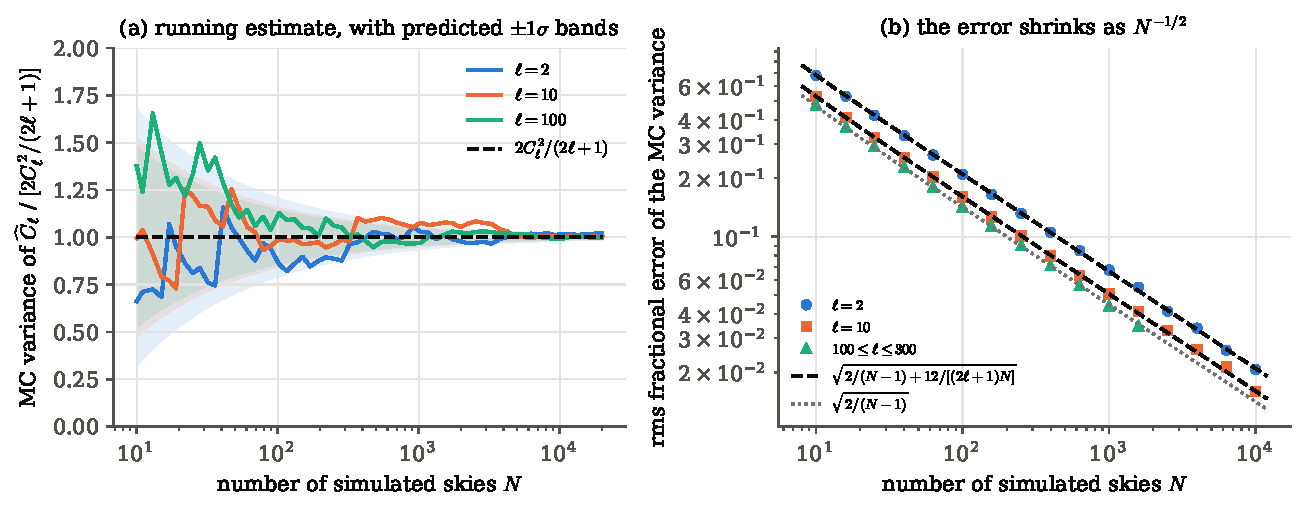
\includegraphics[width=0.98\linewidth]{figures/ch07/mc_variance.pdf}
\caption{(a) Running Monte Carlo estimate of $\Var\Chat$ divided by the cosmic variance
$2\Cell^2/(2\ell+1)$, for $\ell=2$, $10$, $100$, with the predicted $\pm1\sigma$ bands of
\eqref{7b:eq:mc-error}. (b) Measured rms fractional error of the Monte Carlo variance against the
number of skies $N$ per batch. Black dashed: \eqref{7b:eq:mc-error} for $\ell=2$ (upper) and
$\ell=10$ (lower); grey dotted: the Gaussian $\sqrt{2/(N-1)}$. All lines have slope $-1/2$.}
\label{7b:fig:mc-variance}
\end{figure}

\subsection{Different multipoles are independent}
\label{7b:sec:mc-cov}

The third question is about pairs of multipoles. On the full sky, $\Chat$ is a function of the
$2\ell+1$ real numbers at multipole $\ell$ only, and $\widehat C_{\ell'}$ of those at $\ell'$ only.
By \eqref{7b:eq:alm-cov} and Gaussianity, the two sets are independent, so $\Chat$ and $\widehat C_{\ell'}$ are independent for $\ell\neq\ell'$ and
their covariance matrix is diagonal,
\begin{equation}
  \Cov\bigl(\Chat,\widehat C_{\ell'}\bigr)=\frac{2\Cell^2}{2\ell+1}\,\delta_{\ell\ell'} .
  \label{7b:eq:cl-cov}
\end{equation}
This is what made the binning of \eqref{7b:eq:binned} legitimate, and it is the property that a
mask destroys (\cref{7b:sec:what-cl-misses}).

A covariance estimated from $N$ skies is never exactly diagonal, so we need to know what ``zero''
looks like. The answer: the estimated correlation of two independent quantities scatters around
zero with standard deviation $1/\sqrt N$. To see why, take two independent variables, standardise them to $u=(\Chat-\Cell)/\sigma_\ell$ and
$v=(\widehat C_{\ell'}-C_{\ell'})/\sigma_{\ell'}$, and look at the sample correlation coefficient.
For large $N$ the corrections from estimating the means and standard deviations are of relative
order $1/N$, so $r\approx\frac1N\sum_iu_iv_i$, and
\begin{align}
  \Var r
  &\eqby{1}\frac{1}{N^2}\sum_i\E\bigl[u_i^2v_i^2\bigr]
   \eqby{2}\frac{1}{N^2}\,N\,\E[u^2]\,\E[v^2]
   \eqby{3}\frac{1}{N} .
  \label{7b:eq:var-r}
\end{align}
\begin{explain}
  \item The skies are independent and $\E[uv]=0$, so the cross terms $i\neq j$ vanish.
  \item $u$ and $v$ are independent, so the mean of the product is the product of the means.
  \item Both are standardised.
\end{explain}
No step used Gaussianity: the skewed $\chi^2_5$ of the quadrupole gives the same $1/\sqrt N$ as
anything else. So an estimated correlation matrix of truly independent quantities should look
like the identity plus noise of standard deviation $1/\sqrt N$ off the diagonal.

\Cref{7b:fig:mc-correlation}(a) shows the correlation matrix of $\Chat$ for $2\le\ell\le41$
estimated from the first $500$ skies. It is the identity plus a speckle of positive and negative
values. Their standard deviation is $\SBoffSdFiveH$, against $1/\sqrt{500}=\SBoffInvFiveH$. (The
$780$ distinct pairs share variables, so their spread is itself uncertain by a few percent.) With
all $\SBNsim$ skies the spread is $\SBoffSdAll$ against $1/\sqrt N=\SBoffInvAll$, and
\cref{7b:fig:mc-correlation}(b) shows the $N^{-1/2}$ law over two and a half decades. Over all
$\SBnOffBig$ pairs with $2\le\ell<\ell'\le300$ the largest correlation is $\SBoffMaxBig$, about
$4.1/\sqrt N$, the size one expects for the largest of so many Gaussian deviates. The script
computes the matrix with \pyname{np.corrcoef}:
\pyfile[firstline=130,lastline=141,firstnumber=130]{code/ch07/25_mc_cosmic_variance.py}{Off-diagonal correlations of $\Chat$ from the first $N$ skies}
\noindent Line 131 estimates the $40\times40$ correlation matrix from the first $N$ rows; line
132 keeps the off-diagonal elements; lines 140--141 repeat it for all $299$ multipoles with every
sky.

\begin{figure}[htbp]
\centering
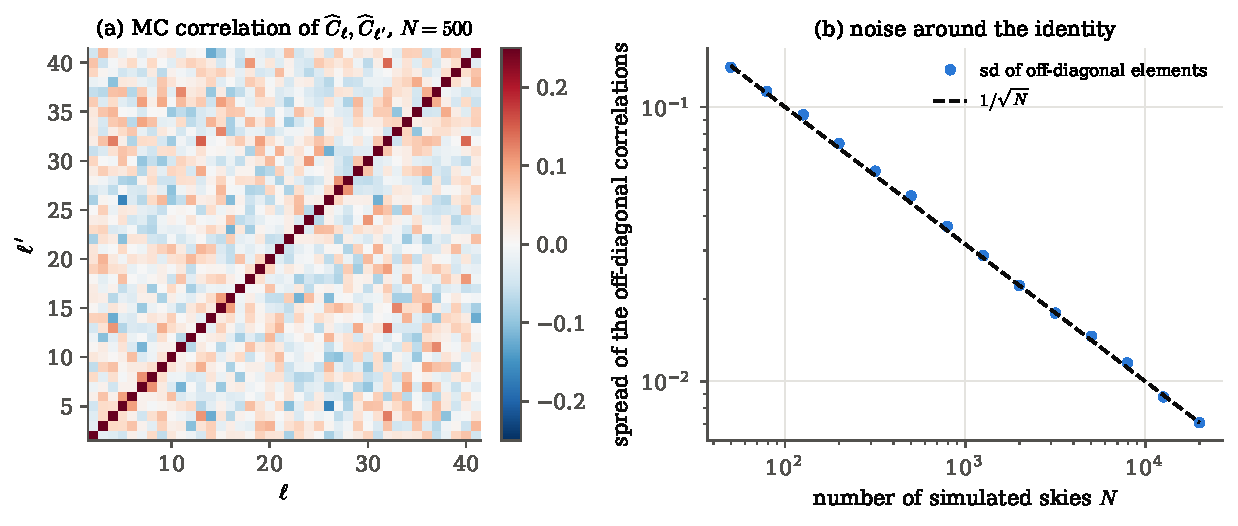
\includegraphics[width=0.98\linewidth]{figures/ch07/mc_correlation.pdf}
\caption{(a) Correlation matrix of $\Chat$ and $\widehat C_{\ell'}$ for $2\le\ell,\ell'\le41$,
estimated from $500$ simulated skies (the colour scale saturates at $\pm0.25$, so the diagonal
$1$ appears as the darkest red). Off the diagonal there is only noise. (b) Standard deviation of
the off-diagonal elements against the number of skies, with the prediction $1/\sqrt N$ of
\eqref{7b:eq:var-r} (black dashed).}
\label{7b:fig:mc-correlation}
\end{figure}

\paragraph{Cross-check with healpy.} Does the library's generator give the same skies as our
from-scratch one? The script draws $\SBhpN$ skies up to $\ell=50$ with
\pyname{healpy.synalm} and measures them with \pyname{healpy.alm2cl}. Two-sample
Kolmogorov--Smirnov tests against our own skies give $p=\SBhpKsTwo$, $\SBhpKsTen$ and $\SBhpKsFifty$
at $\ell=2$, $10$ and $50$, and the healpy variances in units of the cosmic variance are
$\SBhpVrTwo$ ($\ell=2$) and $\SBhpVrFifty$ ($\ell=50$), within the $\pm\sqrt{4.4/3000}\approx4\%$
and $\pm2.6\%$ that \eqref{7b:eq:mc-error} allows for $3000$ skies. The two generators produce the
same skies, statistically.

\begin{inpractice}[Verification here, research instrument next]
These simulations \emph{verify} a result we already had in closed form: the
$\chi^2_{2\ell+1}$ distribution, cosmic variance $2\Cell^2/(2\ell+1)$, and a diagonal covariance.
They test the code and our understanding where the answer is known, and they tell us how many
simulations buy how much precision \eqref{7b:eq:mc-error}.
In research the same loop (draw skies with \pyname{synfast}, push them through the real
pipeline, measure with \pyname{anafast}) is the instrument itself. A real sky is masked, noisy,
beamed and filtered; the pseudo-spectrum is then biased by mode coupling, its covariance is not
diagonal, and no formula gives either exactly. MASTER calibrates the transfer function of the
pipeline and the covariance of the estimate with exactly such simulations \srcref{Hivon}{\S2--3},
\cite{Hivon2002}; Planck's likelihoods are validated on thousands of simulated skies. With
\eqref{7b:eq:mc-error} we know in advance that $1000$ simulations determine a variance to about
$4.5\%$ and a standard deviation to about $2.2\%$. \Cref{ch:08} builds that pipeline.
\end{inpractice}
\section{What $\Cell$ does not see}
\label{7b:sec:what-cl-misses}

The estimator $\Chat$ keeps one number per multipole, the mean of $|\alm|^2$ over $m$. It throws
away the phase of every $\alm$ and the way the power is shared among the $m$. Is anything lost?
For a Gaussian, isotropic sky, no. The covariance \eqref{7b:eq:alm-cov} is then the whole
distribution, the phases are uniformly random, and \cref{ch:03} showed that $\Chat$ is
sufficient for $\Cell$. For any other sky, yes: the phases carry the shapes. In flat space
(\cref{7a:sec:phases}), randomising the Fourier phases of a non-Gaussian field left $P(k)$
untouched and erased every structure in it. The same experiment on the sphere takes a few lines.

\paragraph{Example: hot spots and their phase-scrambled twin.} Can two skies with the same
$\Chat$ look completely different? Paint $\SBphNspot$ Gaussian hot spots of width $4^\circ$ at
random positions on a sky and compute its coefficients. Then build a second sky with the same
$|\alm|$ but new phases. For $m>0$ each $\alm$ is multiplied by a random unit complex number, and
each real $a_{\ell0}$ by a random sign (the only phase a real number can have). The reality
condition \eqref{7b:eq:reality} is respected automatically, because only $m\ge0$ is stored and the
negative $m$ are rebuilt from it. By construction both skies have the same $\Chat$ at every
$\ell$; numerically they agree to $\SBphMaxDiff$. \Cref{7b:fig:phases-maps} shows how different
they look: isolated spots on a flat background, against a featureless Gaussian-looking pattern.
The pixel histograms in \cref{7b:fig:phases-stats}(b) put a number on the difference: the spot sky
has skewness $\SBphSkewA$, its twin $\SBphSkewB$. A test based on $\Chat$ alone could never tell
them apart. (The experiment is \pyname{code/ch07/}\allowbreak\pyname{26_phases_sphere.py}.)

\begin{figure}[htbp]
\centering
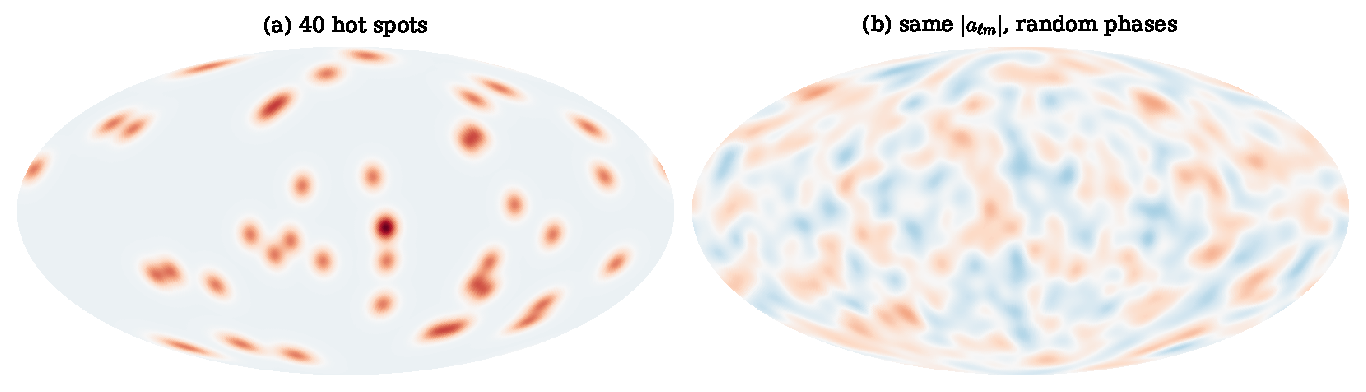
\includegraphics[width=0.98\linewidth]{figures/ch07/phases_maps.pdf}
\caption{(a) A sky made of $\SBphNspot$ hot spots, band-limited to $\ell\le255$. (b) The same
$|\alm|$ with random phases. Same colour scale in both panels. The two skies have identical
$\Chat$ at every multipole.}
\label{7b:fig:phases-maps}
\end{figure}

\begin{figure}[htbp]
\centering
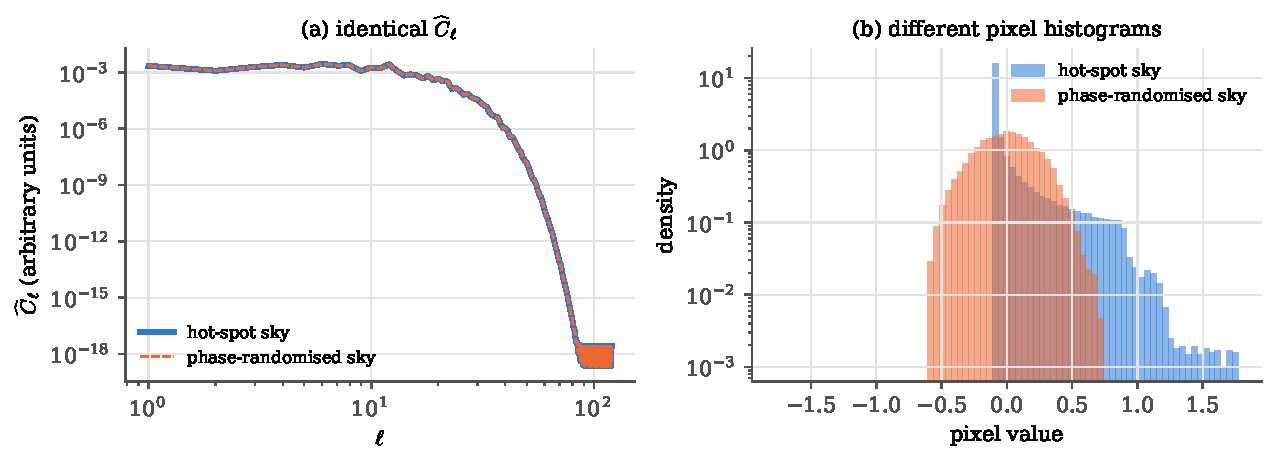
\includegraphics[width=0.95\linewidth]{figures/ch07/phases_stats.pdf}
\caption{(a) $\Chat$ of the two skies of \cref{7b:fig:phases-maps} up to $\ell=120$ (the
$4^\circ$ spots have essentially no power beyond): the curves lie on top of each other. (b) Histograms of their pixel values (logarithmic vertical axis): the spot sky has a
long positive tail, the phase-randomised sky is symmetric and close to Gaussian.}
\label{7b:fig:phases-stats}
\end{figure}

Two things break the clean full-sky picture of this chapter. The first is the sky itself.
Primordial non-Gaussianity ($f_{\rm NL}$, \cref{ch:T1}), lensing and foregrounds put
information into the phases, where $\Cell$ cannot see it; \cref{ch:12} builds summaries that can,
from the shapes of hot and cold regions. The second is the observation: a real map covers only
part of the sky. Let $W(\bm e)$ be the mask, $1$ where we observe and $0$ elsewhere. The
coefficients of the masked sky are $\tilde a_{\ell m}=\int\dd\Omega\,\Theta\,W\,Y^*_{\ell m}$
\srcref{Hivon}{(11)}. Because the mask multiplies the sky, these coefficients mix neighbouring
multipoles, just as multiplying by $1+A\cos\theta$ did in \cref{7b:sec:iso-test}. Their mean square
is then a weighted sum of the true spectrum, $\langle\widetilde C_\ell\rangle=\sum_{\ell'}M_{\ell\ell'}C_{\ell'}$
\srcref{Hivon}{(14)}. The covariance \eqref{7b:eq:cl-cov} is no longer diagonal, the
$\chi^2_{2\ell+1}$ law is gone, and the Monte Carlo loop of \cref{7b:sec:mc} becomes the only way to
get the sampling distribution. That is where \cref{ch:08} begins.

\begin{recap}
\begin{itemize}[itemsep=1pt,leftmargin=1.2em]
  \item The spherical harmonics $Y_{\ell m}$ (eigenfunctions of $\bm L^2$ and $L_z$) are the
        Fourier modes of the sphere; multipole $\ell$ is an angular scale of about $180^\circ/\ell$.
        A sky is $\Theta=\sum\alm Y_{\ell m}$ with $\alm=\int\dd\Omega\,\Theta Y^*_{\ell m}$.
  \item A real sky has $a_{\ell,-m}=(-1)^m\alm^*$: $a_{\ell0}$ is real, and there are $2\ell+1$
        real numbers per $\ell$.
  \item Statistical isotropy makes $\hat C$ commute with all rotations; with $\bm L^2$, $L_z$ and
        $L_\pm$ this gives $\langle\alm a^*_{\ell'm'}\rangle=\Cell\delta_{\ell\ell'}\delta_{mm'}$.
        $C(\vartheta)=\sum(2\ell+1)\Cell P_\ell(\cos\vartheta)/4\pi$. A preferred axis breaks
        both the diagonality and the $m$-independence.
  \item $\Chat=\sum_m|\alm|^2/(2\ell+1)$ is unbiased; $(2\ell+1)\Chat/\Cell\sim\chi^2_{2\ell+1}$
        because $a_{\ell0}$ has variance $\Cell$ and $\mathrm{Re},\mathrm{Im}\,\alm$ have
        $\Cell/2$. Cosmic variance: $\Var\Chat=2\Cell^2/(2\ell+1)$, $63\%$ at the quadrupole.
        Read backwards, the same density is the likelihood
        $\Like(\Cell)\propto\Cell^{-(2\ell+1)/2}e^{-(2\ell+1)\Chat/2\Cell}$.
  \item CAMB solves the linear Boltzmann hierarchy and returns $\Cell=\frac2\pi\int k^2\dd k\,
        P_\zeta g_{T\ell}^2$, an expectation, never a sky. HEALPix has $12N_{\rm side}^2$ equal-area
        pixels on rings; healpy's \texttt{synfast}/\texttt{anafast} go between $\Cell$, $\alm$,
        maps and $\Chat$, accurately below $\ell\approx2N_{\rm side}$.
  \item Monte Carlo with $N$ skies reproduces the $\chi^2$, converges to the cosmic variance with
        fractional error $\sqrt{2/(N-1)+12/[(2\ell+1)N]}$, and gives a correlation matrix equal to
        the identity plus $1/\sqrt N$ noise. This verifies a known result; \cref{ch:08} uses the same
        loop where no formula exists.
  \item $\Chat$ ignores the phases of the $\alm$: skies with the same $\Chat$ can look nothing
        alike.
\end{itemize}
\end{recap}

\subsection*{Reading the literature}
\label{7b:sec:reading-list}

\begin{itemize}[itemsep=2pt,leftmargin=1.2em]
  \item \textbf{Random fields and their two-point statistics.} Hobson et al.\ (eds.),
        \emph{Bayesian Methods in Cosmology}: the pages on parameterising a field by pixels or
        by Fourier modes, where homogeneity makes the Fourier covariance diagonal and a window
        couples the modes, and Chapter~10 (Jaffe) on the CMB as a hierarchical model, with the
        harmonic expansion, the power spectrum, the Wiener filter and the full-sky likelihood
        \srcref{HobsonBMC}{pp.~229--238}. Cowan, \emph{Statistical Data Analysis}, Chapter~1,
        for covariance matrices and their diagonalisation by an orthogonal transformation;
        Wasserman, \emph{All of Statistics}, Chapter~3, for covariance and correlation.
  \item \textbf{Gaussian random fields in cosmology.} Bardeen, Bond, Kaiser and Szalay on the
        statistics of peaks of Gaussian fields \cite{BBKS1986}; Peacock's \emph{Cosmological
        Physics} \cite{Peacock1999} for power spectra, correlation functions and windows; Kaiser
        on clustering in redshift space \cite{Kaiser1987}.
  \item \textbf{The CMB power spectrum and cosmic variance.} Knox on the errors of $\Cell$ from
        noise, beam, sky coverage and cosmic variance \cite{Knox1995}; Hivon et al., MASTER,
        Section~2 for the harmonic expansion, the full-sky estimator and its $\chi^2$, and the
        pseudo-spectrum of a masked sky \cite{Hivon2002}.
  \item \textbf{Computing $\Cell$.} Seljak and Zaldarriaga on line-of-sight integration
        \cite{Seljak1996}; Lewis, Challinor and Lasenby, the CAMB paper \cite{CAMB2000}; Padilla
        et al.\ for a survey of Boltzmann and sampling codes \cite{Padilla2019}; the Planck 2018
        parameters that define the fiducial model \cite{Planck2018VI}, and the Planck tests
        of isotropy \cite{Planck2018VII}. For the physics behind $\Cell$ (the Boltzmann hierarchy,
        transfer functions, acoustic peaks), see the cosmology notes and \cref{ch:T1}.
  \item \textbf{Pixelising the sphere.} G\'orski et al.\ on HEALPix \cite{Gorski2005}.
\end{itemize}

\section*{Chapter summary}
\addcontentsline{toc}{section}{Chapter summary}
\label{7b:sec:summary}

A physical theory of fluctuations predicts the statistics of a field, never the field itself,
and we observe one realisation. Homogeneity and isotropy make the natural modes of the field
uncorrelated: plane waves in flat space, spherical harmonics on the sky. Their variances are
$P(k)$ or $\Cell$, and for a Gaussian field those variances are everything. One realisation offers
only a finite number of independent modes at each scale: $N_{\rm modes}$ in a $k$-shell, or
$2\ell+1$ at a multipole. That number sets an error $\sqrt{2/N_{\rm modes}}$ on every measured
power, and no instrument can reduce it. In the pipeline
\[
  \text{physical model}\to\text{field or dataset}\to\text{summary }S\to
  \boxed{P(S\given\theta)}\to\text{infer physics},
\]
random-field theory supplies the first summaries of a field, $\xi(r)$, $P(k)$ and $\Cell$, and their exact
sampling distributions in the ideal case of a complete, noiseless field; Monte Carlo confirms them.
\Cref{ch:08} adds the mask, the beam and the noise, \cref{ch:09,ch:10} turn the sampling
distribution into parameter constraints, and \cref{ch:12} looks at what the two-point summaries
throw away.

\begin{center}
\small
\renewcommand{\arraystretch}{1.15}
\begin{tabularx}{\linewidth}{@{}>{\raggedright\arraybackslash}p{3.3cm}
                               >{\raggedright\arraybackslash}X
                               >{\raggedright\arraybackslash}p{2.5cm}@{}}
\toprule
\multicolumn{3}{@{}l}{\textbf{Random fields in flat space}}\\
concept & operational meaning & used later in\\\midrule
random field & a random variable at every point, with a joint distribution for any finite set of points; theory predicts its statistics, we see one draw & \cref{ch:08,ch:12}\\
homogeneity, isotropy & all joint distributions unchanged by translations (rotations); the two-point function depends only on the separation & \cref{ch:08,ch:12}\\
correlation function $\xi(r)$ & $\langle\delta(\bm x)\delta(\bm x+\bm r)\rangle$: how strongly the field at two points a distance $r$ apart is related & \cref{ch:10,ch:12}\\
Gaussian random field & all joint distributions Gaussian; mean and $\xi(r)$ determine everything & \cref{ch:08,ch:09,ch:12}\\
power spectrum $P(k)$ & variance of each Fourier mode; Fourier modes of a homogeneous field are uncorrelated; $P$ is the Fourier transform of $\xi$ (Wiener--Khinchin) & \cref{ch:08,ch:10}\\
simulating a field & colour white noise by $\sqrt{P(k)}$ in Fourier space and transform back (FFT) & \cref{ch:08,ch:12}\\
ergodicity, sample variance & a spatial average replaces the ensemble average when distant regions are nearly independent; a $k$-shell with $N_{\rm modes}$ modes gives $\Delta P/P=\sqrt{2/N_{\rm modes}}$ & \cref{ch:08,ch:10}\\
smoothing & a beam, pixel or counting cell multiplies $P(k)$ by $|W(k)|^2$ & \cref{ch:08,ch:12}\\
spectral moments $\sigma_j$ & integrals of $k^{2j}P(k)$ (with the window): the variance of the field, of its gradient and the typical spacing of its features & \cref{ch:12}\\
phases & $P(k)$ keeps the amplitudes and discards the phases; phases hold the shapes of non-Gaussian fields & \cref{ch:12}\\
\bottomrule
\end{tabularx}
\end{center}

\begin{center}
\small
\renewcommand{\arraystretch}{1.15}
\begin{tabularx}{\linewidth}{@{}>{\raggedright\arraybackslash}p{3.3cm}
                               >{\raggedright\arraybackslash}X
                               >{\raggedright\arraybackslash}p{2.5cm}@{}}
\toprule
\multicolumn{3}{@{}l}{\textbf{Fields on the sphere}}\\
concept & operational meaning & used later in\\\midrule
spherical harmonics, $\alm$ & eigenfunctions of $\bm L^2$, $L_z$; $\alm=\int\dd\Omega\,\Theta Y^*_{\ell m}$; multipole $\ell\leftrightarrow$ angle $180^\circ/\ell$ & \cref{ch:08,ch:12}\\
reality condition & $a_{\ell,-m}=(-1)^m\alm^*$; $a_{\ell0}$ real; $2\ell+1$ real numbers per $\ell$, $(\ell_{\max}+1)^2$ in all; store $m\ge0$ only & \cref{ch:08}\\
isotropy in harmonic space & $\langle\alm a^*_{\ell'm'}\rangle=\Cell\delta_{\ell\ell'}\delta_{mm'}$, from $[\hat C,\bm L]=0$ and the ladder operators; a preferred axis couples $\ell$ to $\ell\pm1$ & \cref{ch:08,ch:09}\\
$C(\vartheta)$ and $\Cell$ & $C(\vartheta)=\sum_\ell\frac{2\ell+1}{4\pi}\Cell P_\ell(\cos\vartheta)$, $\Cell=2\pi\int\dd\cos\vartheta\,P_\ell C$; point variance $\sum(2\ell+1)\Cell/4\pi$ & \cref{ch:08,ch:12}\\
full-sky estimator $\Chat$ & mean of $|\alm|^2$ over $m$; unbiased, sufficient, maximum likelihood & \cref{ch:08,ch:09,ch:10}\\
$\chi^2_{2\ell+1}$ law & $(2\ell+1)\Chat/\Cell\sim\chi^2_{2\ell+1}$: one real $a_{\ell0}$ of variance $\Cell$, $2\ell$ real and imaginary parts of variance $\Cell/2$; skewed at low $\ell$ & \cref{ch:08,ch:09}\\
cosmic variance & $\Var\Chat=2\Cell^2/(2\ell+1)$ (the Cram\'er--Rao bound); binned: divide by $\Delta\ell$; with noise and sky fraction, $(\Cell+N_\ell/B_\ell^2)\sqrt{2/[(2\ell+1)\Delta\ell\fsky]}$ & \cref{ch:08,ch:10}\\
likelihood of $\Cell$ & $\Like\propto\Cell^{-(2\ell+1)/2}\exp[-(2\ell+1)\Chat/2\Cell]$: broad and lopsided at low $\ell$ & \cref{ch:09,ch:10}\\
CAMB & solves the linear Boltzmann hierarchy, line of sight; $\Cell=\frac2\pi\int k^2\dd k\,P_\zeta g_{T\ell}^2$; call with \texttt{raw\_cl=True}, $\mu$K$^2$ & \cref{ch:08,ch:09,ch:10}\\
HEALPix and healpy & $N_{\rm pix}=12N_{\rm side}^2$ equal areas on rings, pixel $58.6^\circ/N_{\rm side}$; \texttt{synalm}, \texttt{alm2map}, \texttt{map2alm}, \texttt{alm2cl}; trust $\ell\lesssim2N_{\rm side}$; pixel window & \cref{ch:08,ch:12}\\
Monte Carlo of $\Chat$ & simulate skies, histogram $\Chat$; MC variance error $\sqrt{2/(N-1)+12/[(2\ell+1)N]}$; off-diagonal correlations $\pm1/\sqrt N$ & \cref{ch:08,ch:09}\\
verification vs research & here the simulation checks a closed-form answer; with a mask, noise and a beam it is the only way to the sampling distribution & \cref{ch:08}\\
what $\Cell$ misses & the phases of the $\alm$: equal $\Chat$, different shapes and pixel histograms & \cref{ch:12}\\
\bottomrule
\end{tabularx}
\end{center}
  